%Przykładowy plik ułatwiający złożenie projektu dyplomowego inżynierskiego.
%UWAGA: Generowany napis na stronie tytułowej o treści PROJEKT DYPLOMOWY INŻYNIERSKI został zaproponowany przeze mnie i nie jest, póki co, potwierdzony przez władze wydziału. Przed ostatecznym oddaniem tak złożonej pracy należy upewnić się jaka powinna być treść tego napisu. W momencie gdy uzyskam informację na temat treści tego napisu, dokonam niezbędnych zmian w źródłach.

\documentclass[eng,printmode]{mgr}
%opcje klasy dokumentu mgr.cls zostały opisane w dołączonej instrukcji

%poniżej deklaracje użycia pakietów, usunąć to co jest niepotrzebne
\usepackage{polski} %przydatne podczas składania dokumentów w j. polskim
%\usepackage[polish]{babel}%alternatywnie do pakietu polski, wybrać jeden z nich
\usepackage[utf8]{inputenc} %kodowanie znakĂłw, zaleĹĽne od systemu
\usepackage[T1]{fontenc} %poprawne składanie polskich czcionek

%pakiety do grafiki
\usepackage{graphicx}
%\usepackage{subfigure}
\usepackage{psfrag}

%pakiety dodające dużo dodatkowych poleceń matematycznych
\usepackage{amsmath}
\usepackage{amsfonts}

%pakiety wspomagające i poprawiające składanie tabel
%\usepackage{supertabular}
\usepackage{array}
\usepackage{tabularx}
\usepackage{hhline}

\usepackage{mathtools}
\usepackage{listings}
\usepackage{rotating}

%pakiet wypisujący na marginesie etykiety równań i rysunków zdefiniowanych przez \label{}, chcąc wygenerować finalną wersję dokumentu wystarczy usunąć poniższą linię
%\usepackage{showlabels}

%definicje własnych poleceń
\newcommand{\R}{I\!\!R} %symbol liczb rzeczywistych, działa tylko w trybie matematycznym
\newtheorem{theorem}{Twierdzenie}[section] %nowe otoczenie do składania twierdzeń

%dane do złożenia strony tytułowej
\title{Detekcja aktywności mówcy w systemach automatycznego rozpoznawania mowy}
\engtitle{Voice activity detection in automatic speech recognition systems}
\author{Paulina Szczerbak}
\supervisor{Prof. dr hab. inż. Ryszard Makowski}
%\guardian{dr hab. inż. Imię Nazwisko Prof. PWr, I-6} %nie używać jeśli opiekun jest tą samą osobą co prowadzący pracę

%\date{2008} %standardowo u dołu strony tytułowej umieszczany jest bieżący rok, to polecenie pozwala wstawić dowolny rok

%poniżej jest lista kierunków i specjalności na wydziale elektroniki, należy wybrać właściwe lub dopisać jeśli nie ma odpowiednich
\field{Automatyka i Robotyka}
\specialisation{Technologie informacyjne w systemach automatyki (ART)}

%tutaj zaczyna się właściwa treść dokumentu
\begin{document}
\bibliographystyle{plabbrv} %tylko gdy uĹĽywamy BibTeXa, ustawia polski styl bibliografii

\maketitle %polecenie generujące stronę tytułową
%\dedication{6cm}{Dla mamy i taty heheheheheh xD \texttt{$\backslash$dedykacja}}

\tableofcontents %spis treści

%poniżej znajduje się przykładowa treść dalszej części dokumentu, zainteresowanych zachęcam do rozszyfrowania frazy "Lorem ipsum" :)
\chapter{Wstęp}
Celem niniejszej pracy jest zaprezentowanie oraz ocena skuteczności wybranych metod detekcji aktywności mówcy (VAD) w systemach automatycznego rozpoznawania mowy. W toku pracy, wspomniane metody detekcji zostały zaimplementowane w języku C++. W efekcie możliwe było porównanie tych metod pod względem dokładności detekcji w separowanych wyrazach oraz dla ciągów słów. Badania zostały przeprowadzone dwukrotnie - pierwsze przy minimalnym zaszumieniu sygnału, a drugie przy dużo wyższym poziomie szumu. \vspace{3mm}

Rozdział 2: skrócony opis procesu wytwarzania mowy przez człowieka. Zaprezentowano, w jaki sposób działa aparat mowy oraz z jakich elementów się składa. Omówiona zostaje między innymi istota sprzężeń zwrotnych w organiźmie podczas wytwarzania mowy. Na koniec pokazano przydatne narzędzia do analizowania sygnału mowy - wykresy sygnału w dziedzinie czasu oraz w dziedzinie częstotliwości.\vspace{3mm}

Rozdział 3: problem detekcji aktywności mówcy pod kątem jego celowości i sposobu wykorzystania. W tym rodziale opisane są również wybrane algorytmy, które zostały przebadane w dalszej części pracy. \vspace{3mm}

Rozdział 4: sposób oceny wyników oraz wyniki. Zawiera  wyniki detekcji dla pojedynczych słów oraz całych ciągów. Przypadek ciągu słów został rozpatrzony w warunkach małego oraz dużego zaszumienia sygnału. \vspace{3mm}

Podsumowanie: analiza porównawcza skuteczności wybranych algorytmów i ich ocena.

Dodatek A: niektóre aspekty implementacyjne każdego z algorytmów.

\chapter{Generowanie sygnału mowy}
 \section{Mowa w życiu człowieka}
 
 Mowa w życiu ludzi stanowi podstawę komunikacji interpersonalnej. Jest ona sygnałem akustycznym, czyli rozważany jest zakres częstotliwości słyszanych przez człowieka, to jest od 20Hz do 16kHz. Zatem mowa to nic innego jak system artykułowanych dźwięków, które układają się zgodnie z konwencją wybranego języka. Pełni ona funkcję nie tylko komunikacyjną (przekazywanie informacji drugiej osobie o tym, co doświadczyliśmy, czy czego się dowiedzieliśmy), ale również ekspresyjną (można w niej zawrzeć informacje o emocjach nadawcy) oraz regulacyjną (wydawanie i przyjmowanie dyspozycji). 
 
 
 \section{Biologiczny proces generowania mowy}
 Wszelkie metody przetwarzania sygnału mowy muszą uwzględniać właściwości sygnału, które są uzależnione od sposobu, w jaki jest on wytwarzany. Niegdyś generowanie sygnałów mowy było domeną jedynie organizmu człowieka, czyli systemu naturalnego. W celu stworzenia systemu, który w jakiś sposób operuje na sygnałach mowy, czyli np. syntezatora mowy, systemu generującego sygnały mowopodobne, systemu automatycznego rozpoznawania mowy czy detekcji aktywności mówcy, należy mieć przynajmniej podstawową wiedzę na temat systemu naturalnego - czyli wiedzę o tym, w jaki sposób funkcjonuje aparat mowy człowieka.
 
 Wytwarzanie mowy przez człowieka jest procesem niezwykle skomplikowanym, który ma swój początek w mózgu, gdzie następuje konstrukcja wypowiedzi. Później następuje sformułowanie fonetyki i artykulacja poprzez aparat mowy. Ponadto, w procesie generowania mowy można wyróżnić cztery pomniejsze etapy \cite{Zemlin}:
	 
	 - proces psychologiczny - wymyślenie i skonstruowanie wypowiedzi,
	 
	 - proces neurologiczny - pobudzenie przez układ nerwowy mięśni, które biorą udział w wytwarzaniu mowy,
	 
	 - proces fizjologiczny - proces kształtowania dźwięków mowy ludzkiej,
	 
	 - proces aerodynamiczny - drgania i przepływ powietrza przez aparat mowy. 
  
  Pierwszym narządem wchodzącym w skład traktu głosowego człowieka są płuca - dostarczają one powietrze do procesu artykulacji, są źródłem zmian ciśnienia akustycznego. Organ mowy człowieka jest napędzany przez wydychane powietrze. W przypadku dźwięcznych fragmentów mowy, powietrze jest prowadzone przez oskrzela i tchawicę do krtani, a drgające w niej struny głosowe modyfikują ciśnienie. Następnie, dzięki wnękom rezonansowym, tworzonym przez język, podniebienie, zęby oraz wargi, dźwięk ten jest modulowany. Natomiast bezdźwięczne fragmenty mowy mają charakter szumowy, w trakcie ich trwania struny głosowe pozostają nieruchome.  

\begin{figure}
	Niezwykle ważną rolę przy formowaniu tych wnęk, odgrywają ruchy żuchwy i policzków. Podczas generowania głosek nosowych zamknięta jama ustna spełnia rolę bocznika akustycznego, a dzięki odpowiedniemu ustawieniu języczka podniebienia miękkiego, fala dźwiękowa jest emitowana przez jamę nosową i nozdrza. Struktura traktu głosowego jest przedstawiona schematycznie na rysunku 2.1. \cite{Zemlin}
	\begin{center}
		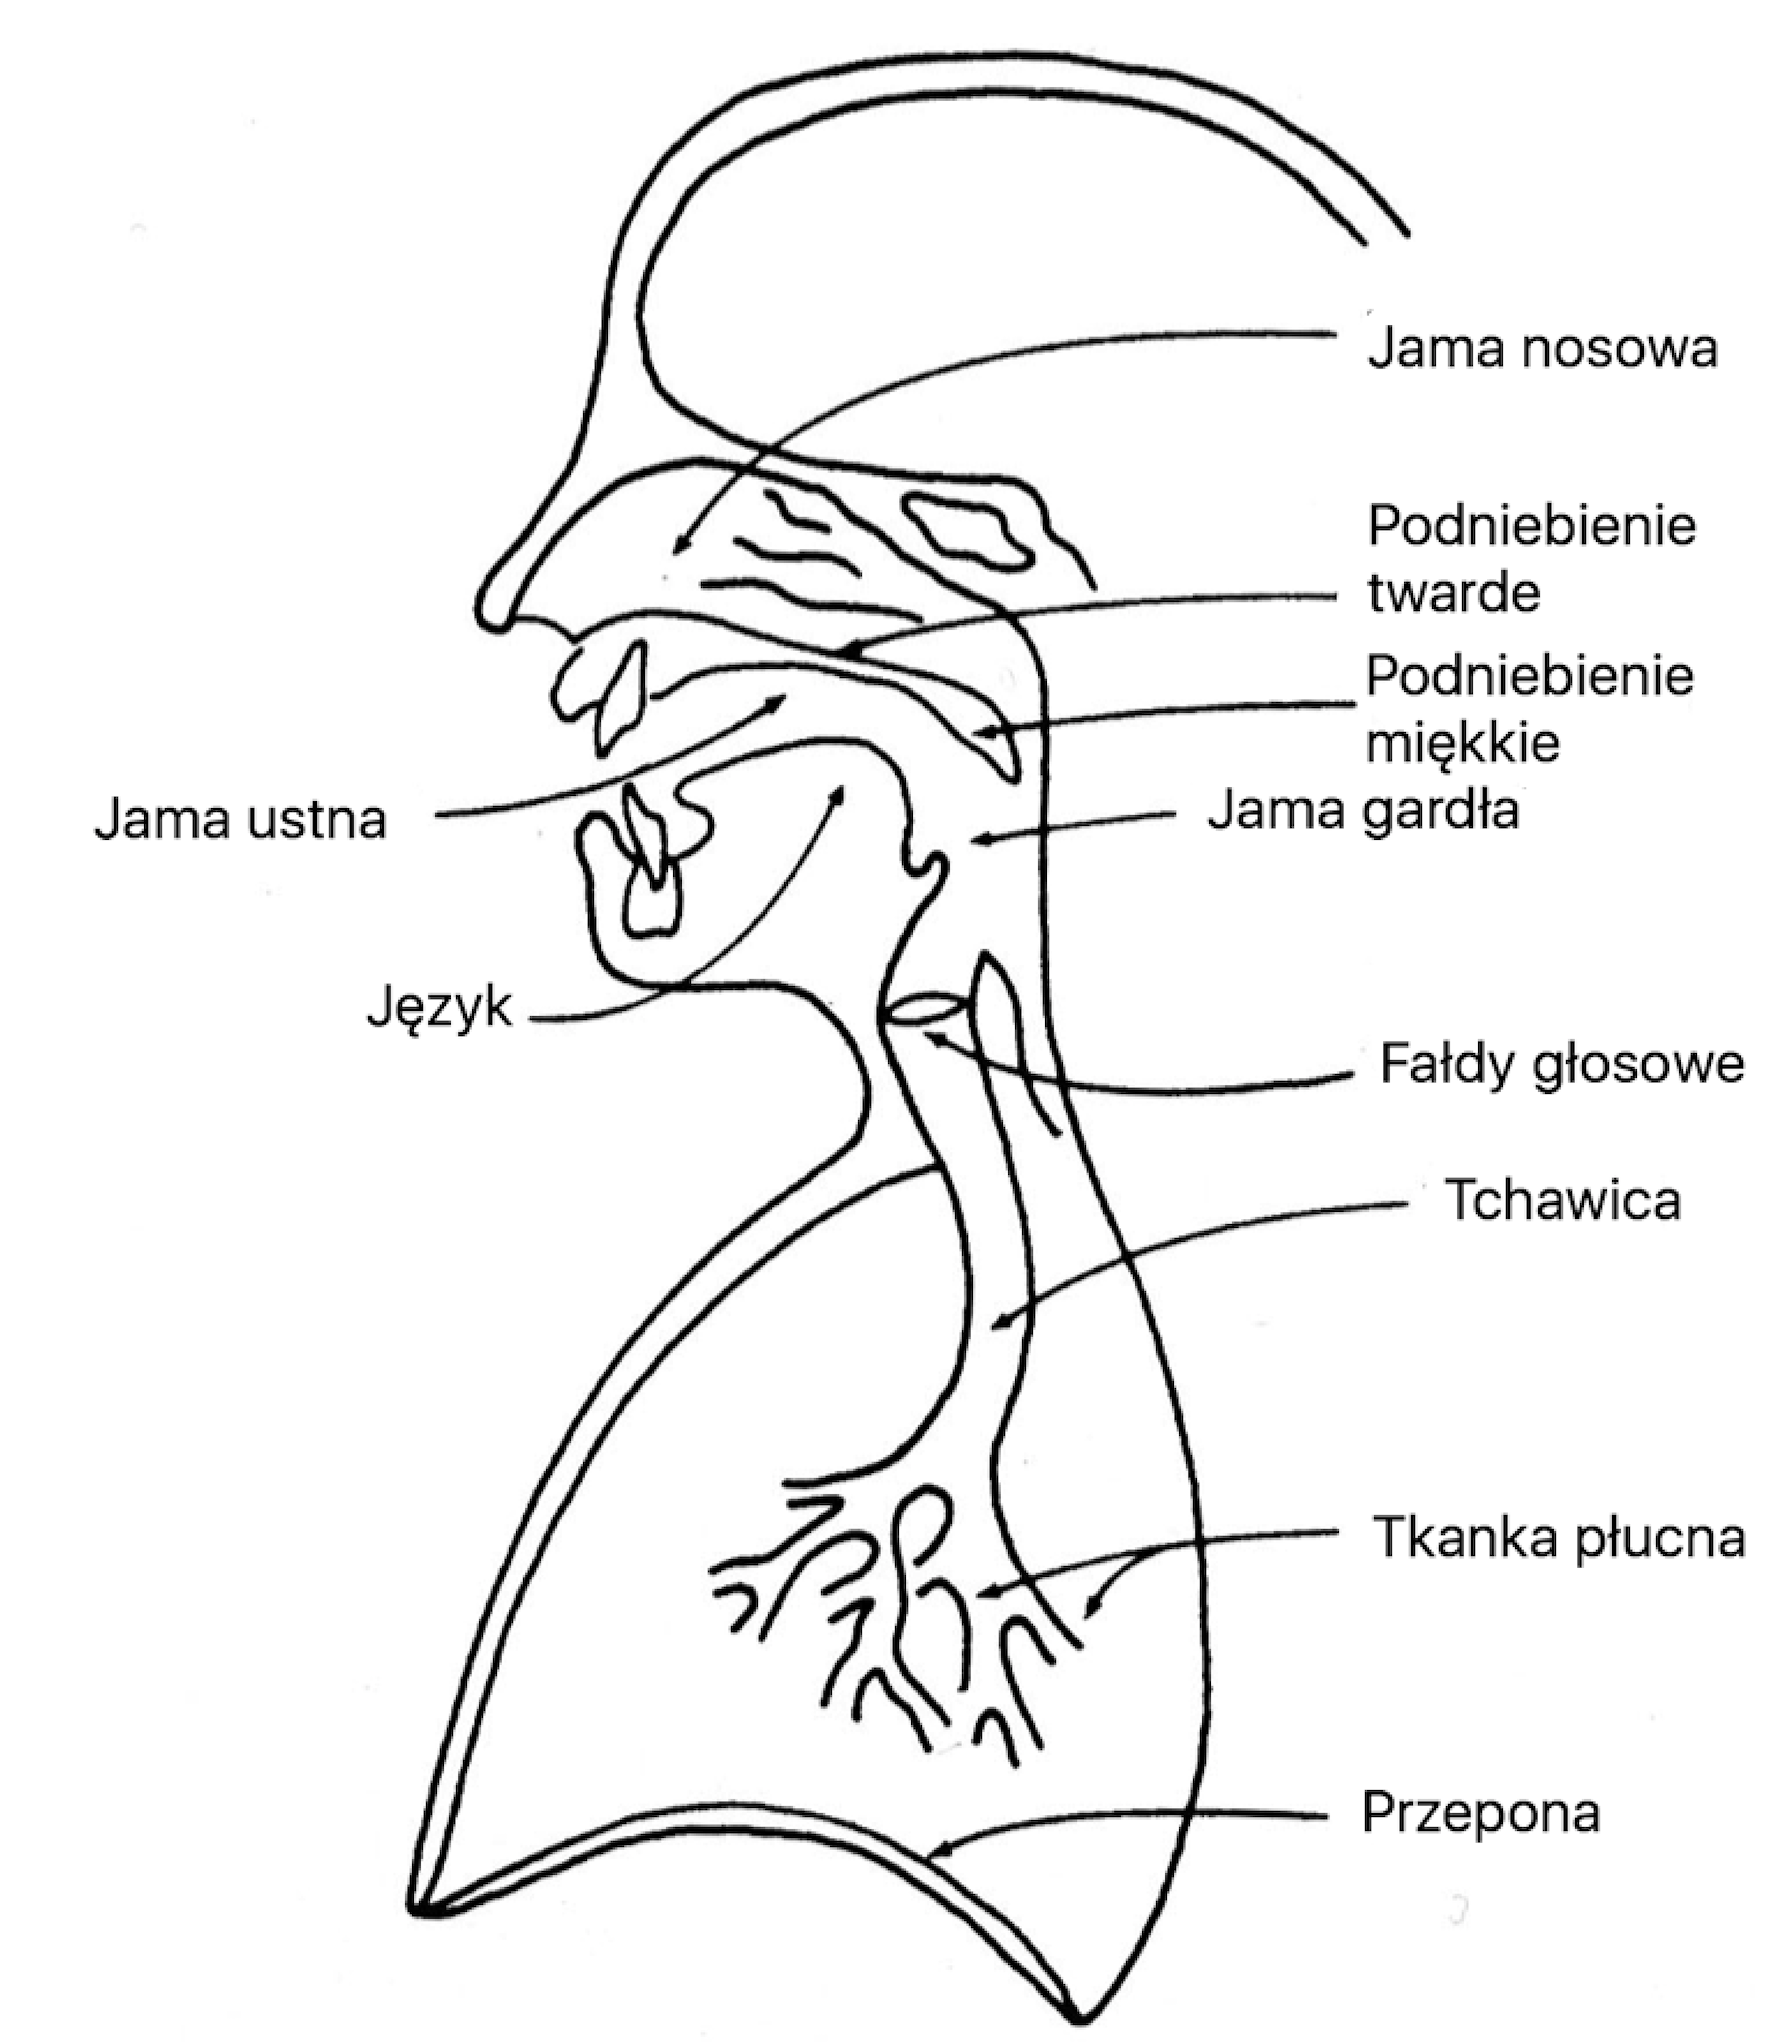
\includegraphics[scale=0.25]{speechmechpl.png}
		\caption{Aparat mowy człowieka}\vspace{5mm}
	\end{center}

	 Ponadto, sterowanie całym systemem generowania mowy jest bardzo złożone i w dużej mierze opiera się na licznych sprzężeniach zwrotnych. Główną rolę odgrywa tutaj sprzężenie zwrotne, które poddaje jakość wydawanych dźwięków bezpośredniej ocenie poprzez organ słuchu. Dzięki temu proces artykulacji jest odpowiednio kontrolowany. Istotę tego sprzężenia zwrotnego potwierdzają trudności z mową wśród ludzi głuchych oraz ludzi słyszących, którzy tymczasowo przebywają w trudnych warunkach środowiskowych, które uniemożliwiają słyszenie własnego głosu. Schemat jego działania zaprezentowano na Rysunku 2.2.\vspace{5mm}
 
	 \begin{center}
	 	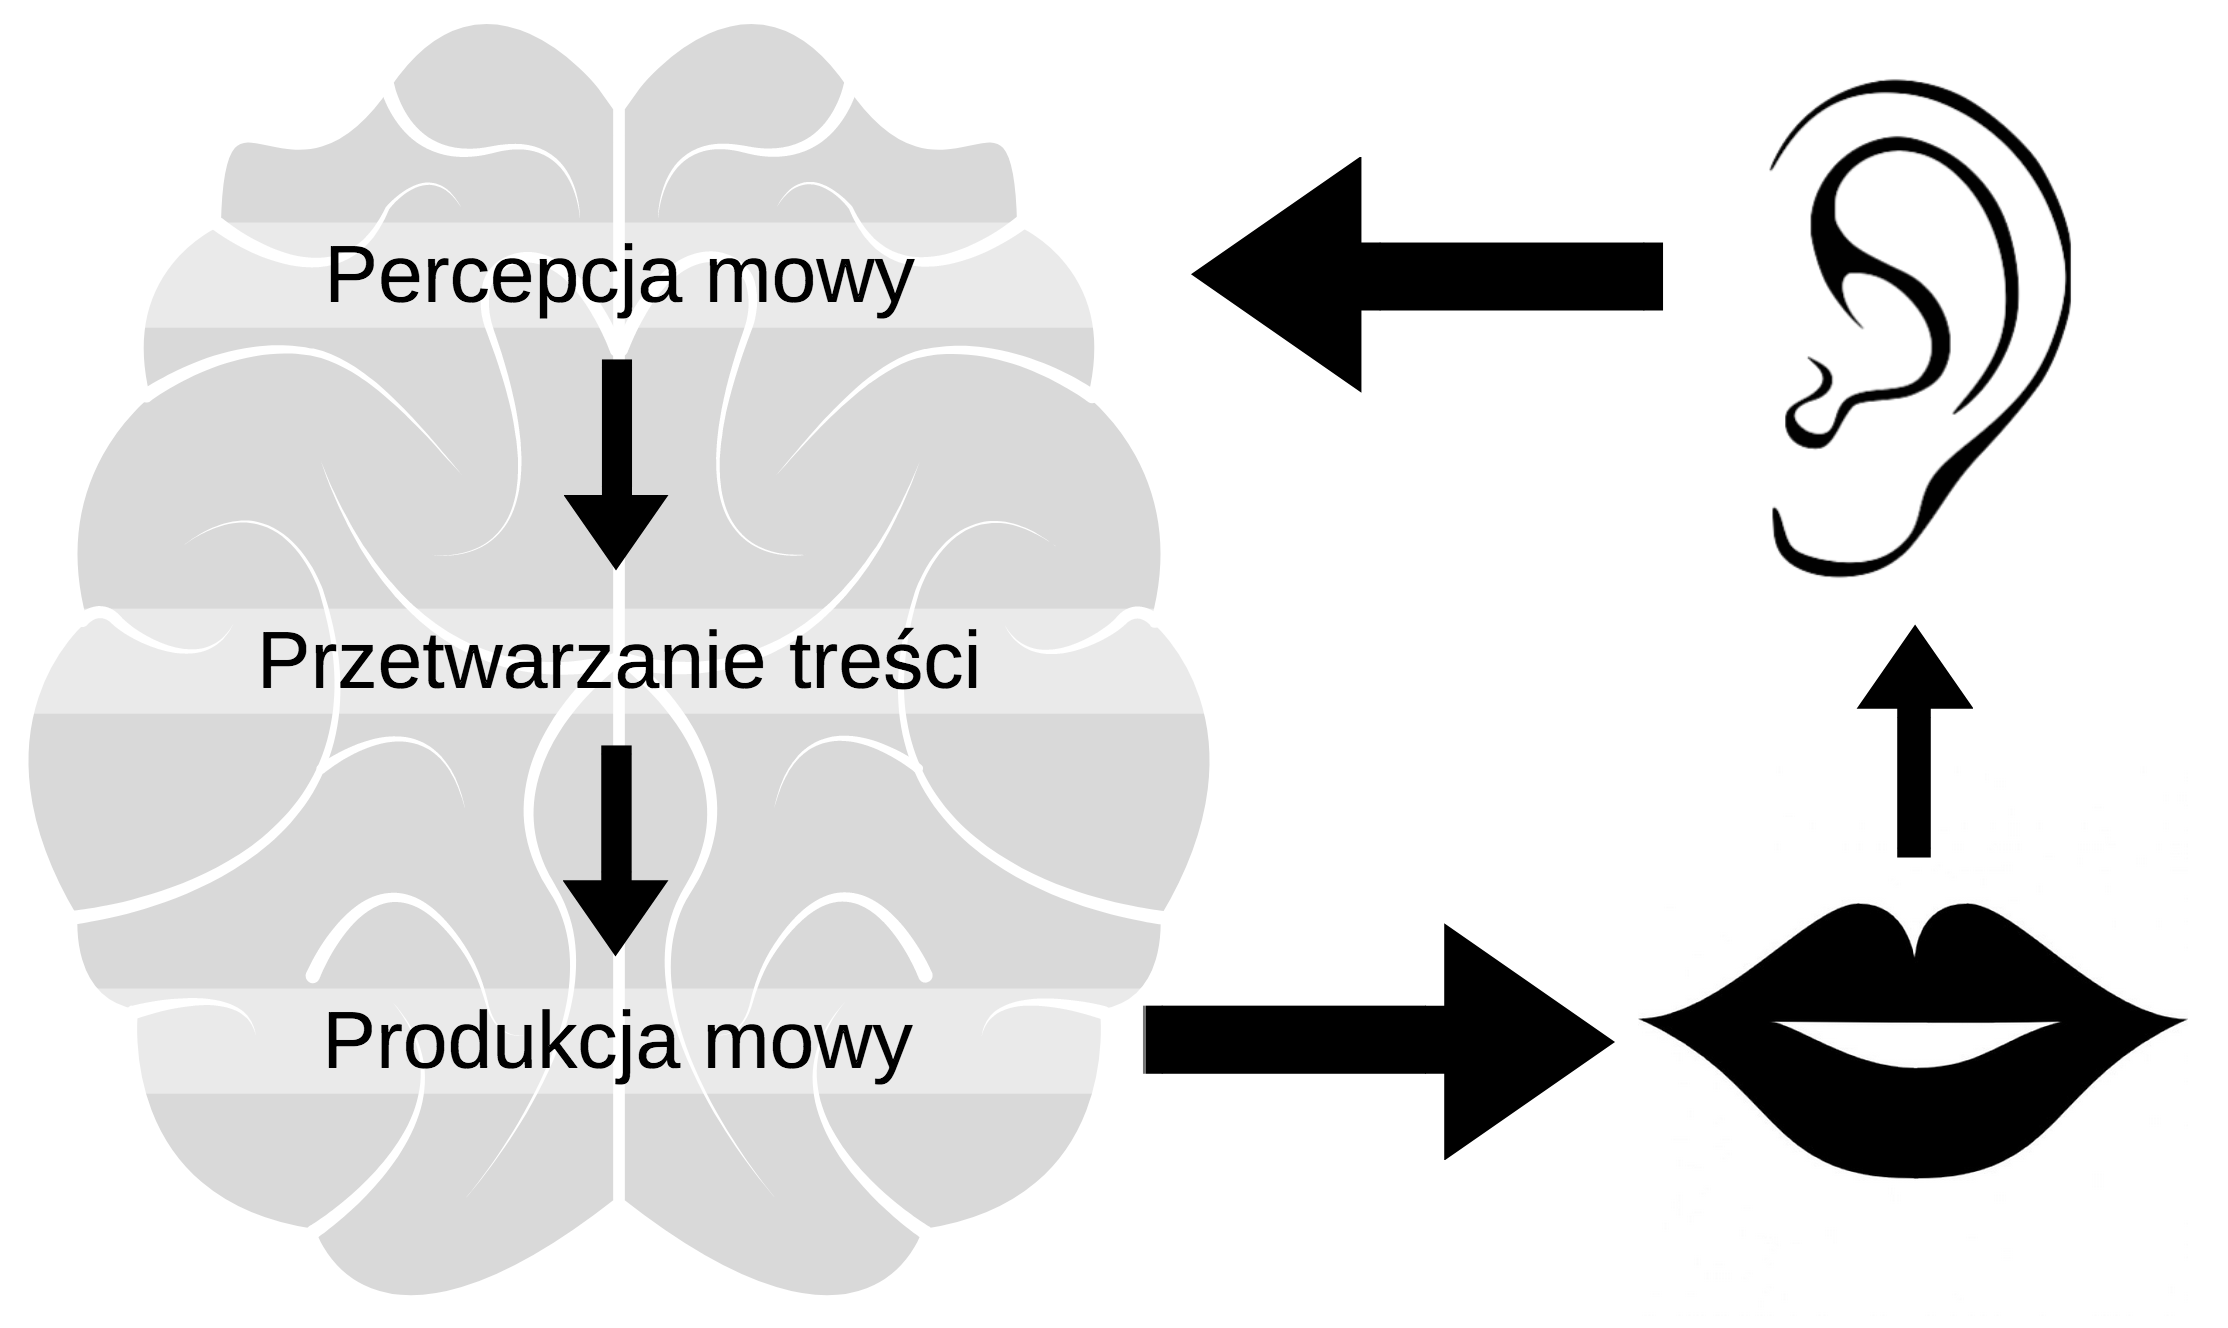
\includegraphics[scale=0.25]{feedback.png}
	 	\caption{Sprzężenie zwrotne w wytwarzaniu mowy} 	
	 \end{center}
 \end{figure}
 
\begin{figure}
 	\section{Sygnał w dziedzinie czasu oraz w dziedzinie częstotliwości}
	Powstawanie głosu jest bardzo złożonym zjawiskiem akustyczno - mechanicznym, a jego bazowym składnikiem jest dźwięk. W kategoriach fizycznych dźwięk tworzą drgania mechaniczne, a w organiźmie człowieka takim generatorem drgań jest krtań. Charakter tego dźwięku, zwany też tonem krtaniowym (lub tonem podstawowym), zależy od właściwości fałdów głosowych - ich długości, napięcia, elastyczności i masy oraz od charakteru przepływu powietrza. Ton krtaniowy ma określoną wysokośc i natężenie, ale sam w sobie jest słaby i bezbarwny. Nabiera odpowiedniej siły i barwy dopiero poprzez przejście przez wyższe partie traktu głosowego. Mowa dźwięczna wyróżnia się okresowością - jest bowiem powieleniem tonu krtaniowego.
	
	 Dzięki analizie sygnału w dziedzinie czasu - Rysunek 2.3 - można w prosty sposób wyróżnić dźwięczne fragmenty mowy dzięki regularnie powtarzających się maksimach. 
	 
	 Najważniejszym jednak narzędziem do analizowania mowy, jest jego widmo częstotliwościowe - czyli przedstawienie sygnału w dziedzinie częstotliwości, które można otrzymać przy pomocy transformaty Fouriera. Przypada ono na zakres ok 100-8000Hz. Przykład został zaprezentowany na Rysunku 2.4 [].
 	\begin{center}
 		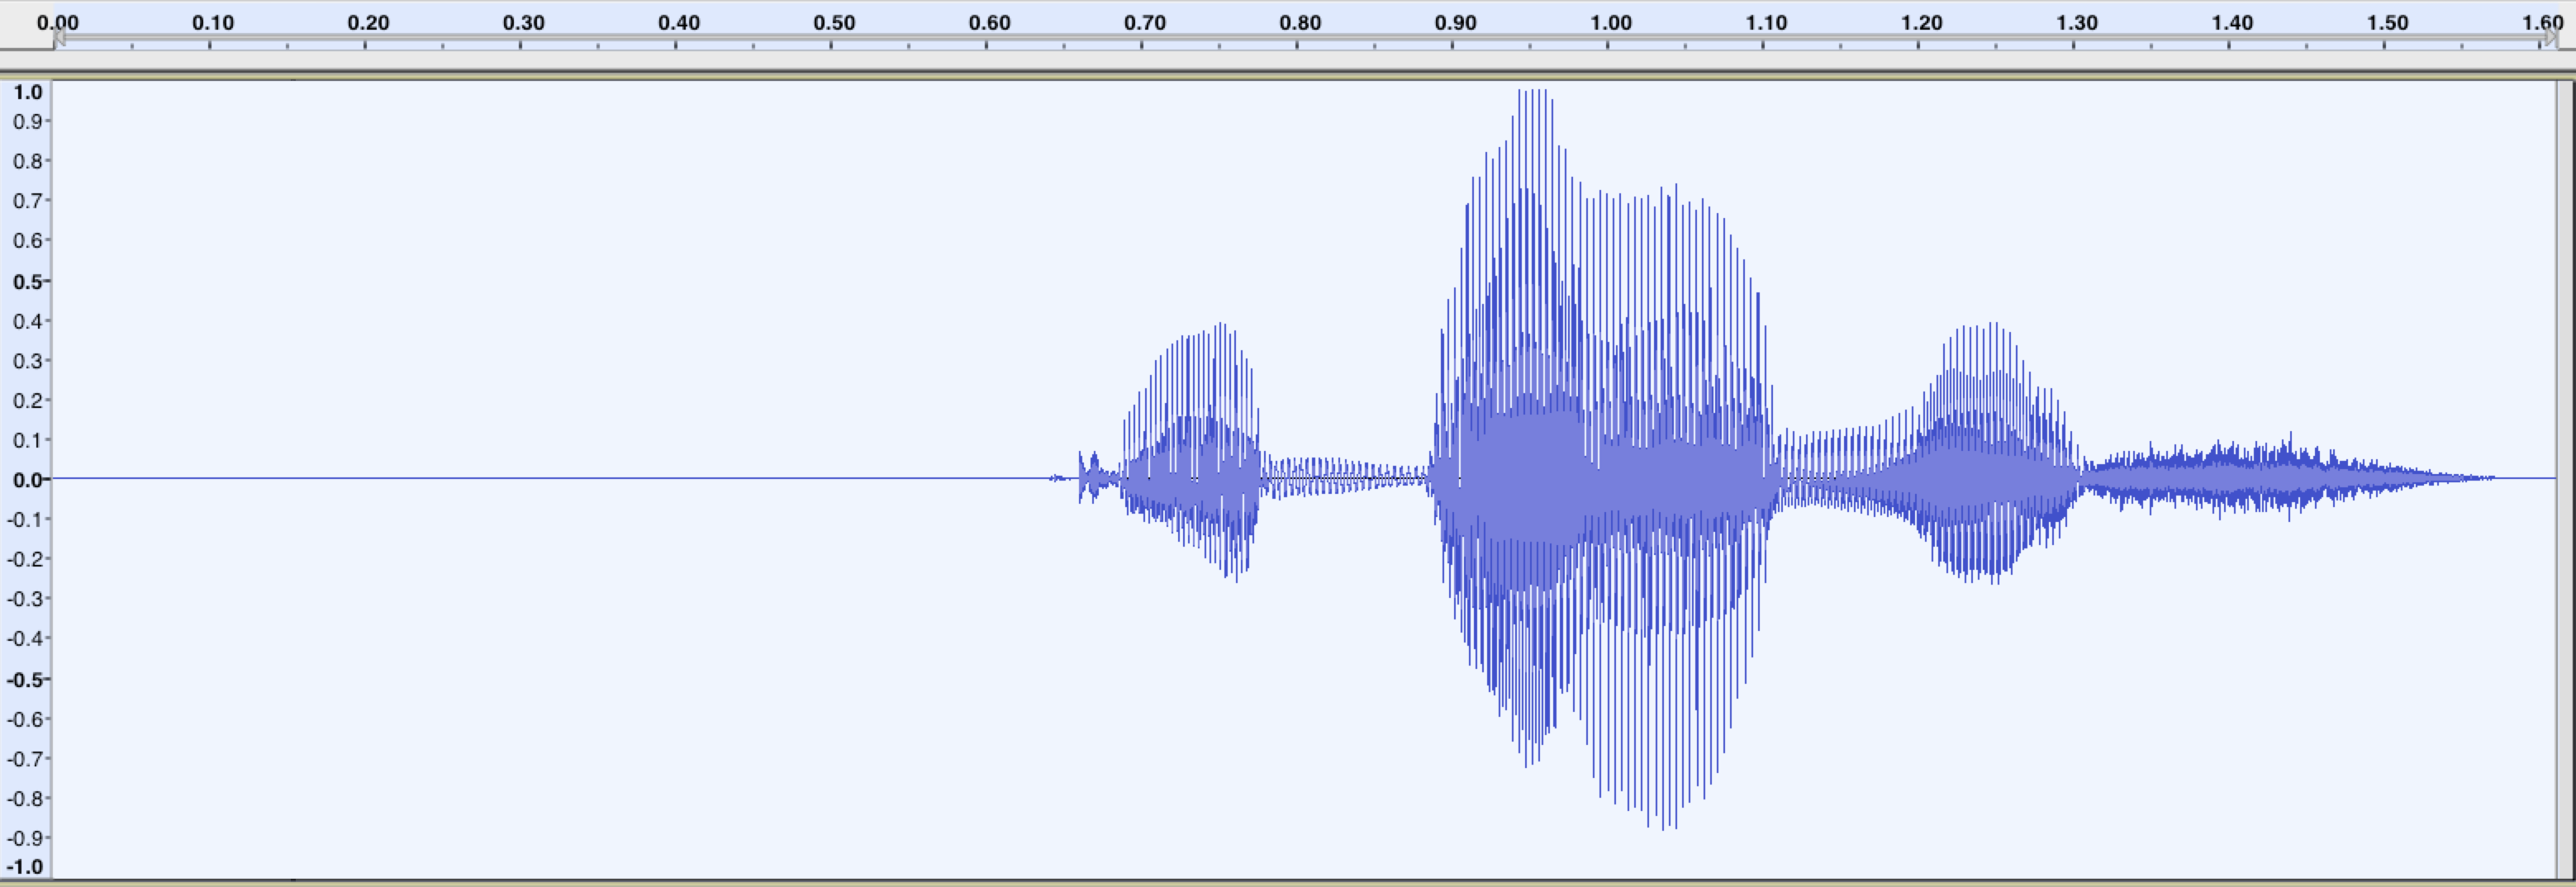
\includegraphics[scale=0.3]{kabanosTime.png}
 		\caption{Przebieg sygnału w dziedzinie czasu dla słowa \emph{kabanos}}\vspace{5mm}
 		
 		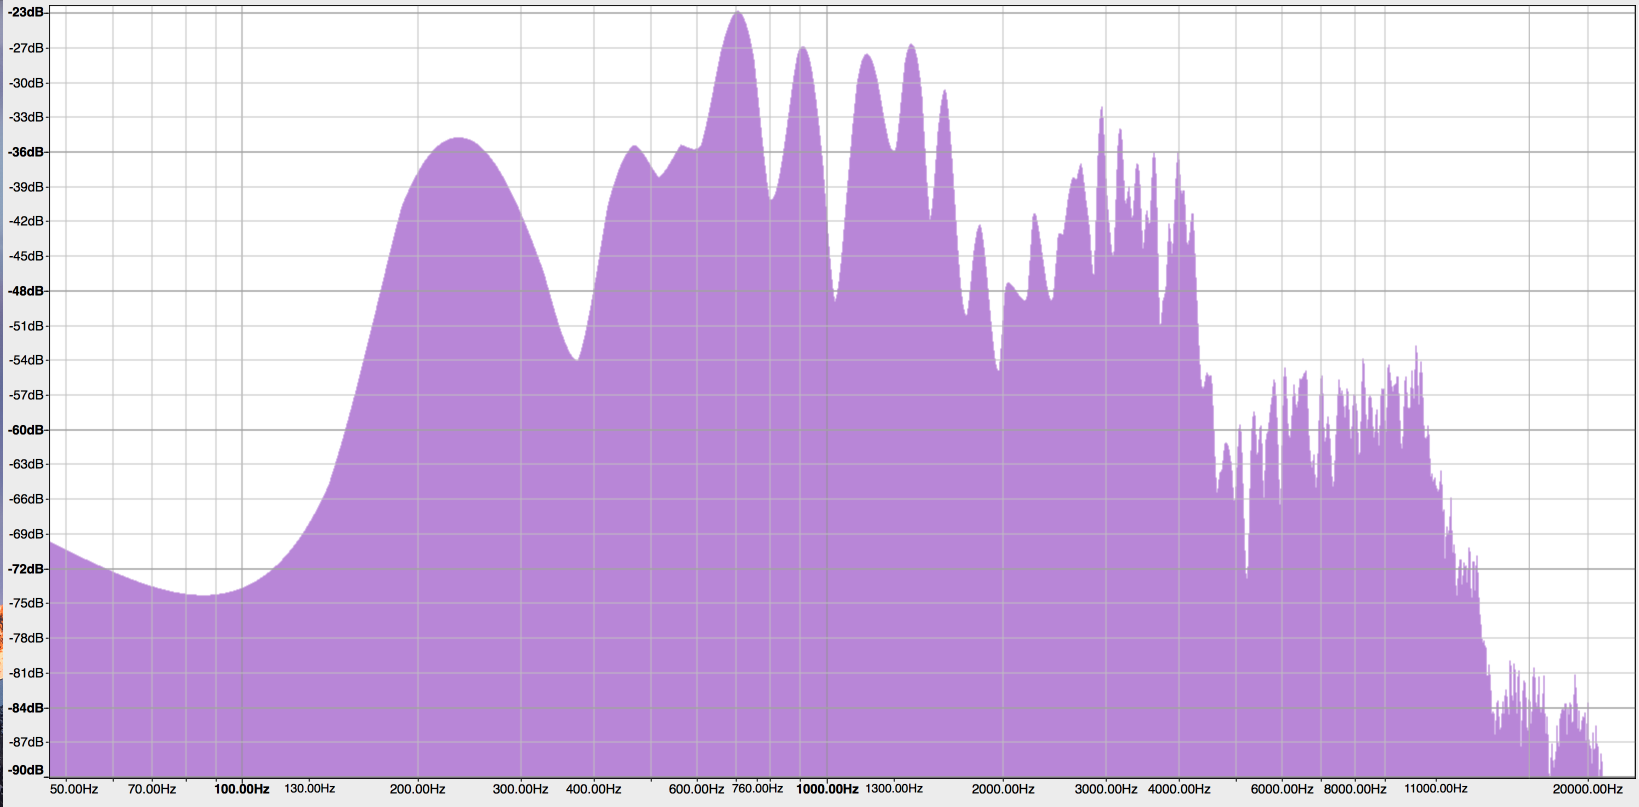
\includegraphics[scale=0.5]{kabanosSpectrum.png}
 		\caption{Widmo sygnału dla słowa \emph{kabanos}}\vspace{5mm}
 	\end{center}
\end{figure}
  
 
\chapter{Wybrane algorytmy detekcji aktywności mówcy}
 \section{Czym jest detekcja aktywności mówcy}
 
 Detekcja aktywności mówcy (Voice Activity Detection - VAD) jest powszechnie stosowana w systemach automatycznego rozpoznawania mowy. Podczas rejestrowania wypowiedzi do późniejszego przetwarzania jej przez system ARM, zostaje zarejestrowana cała wypowiedź mówcy, włącznie z częścią, która nie zawiera mowy. Z kolei fragmenty, w których jest zawarty sygnał mowy, nazywamy fragmentami aktywności mówcy. Aktywnością mówcy nazywa się emitowny przez niego dźwięk. Zawartość semantyczna wypowiedzi jest zawarta w głównej mierze we fragmentach, kiedy mówca jest aktywny (aczkolwiek występowanie przerw też jest informacyjne). Analizowanie całego  zarejestrowanego sygnału mowy, bez wykorzystania systemu VAD, jest oczywiście możliwe, aczkolwiek niepotrzebnie zwiększa czas obliczeń oraz istnieje prawdopodobieństwo, że fragment, gdy mówca nie jest aktywny, zostanie błędnie zaklasyfikowany jako jakiś konkretny fonem - zatem w dużej mierze może popsuć jakość rozpoznania. Detekcja aktywności mówcy w ogólnym przypadku zakłada, że sygnał może występować w dwóch stanach: tylko szum (brak sygnału mowy), szum + sygnał mowy. Korzystając z zagadnienia hipotez ze statystyki, możemy pierwszy stan oznaczyć jako hipotezę $H_{0}$, a drugi jako $H_{1}$, dzięki czemu możemy przedstawić to w następujący sposób \cite{prof}:
 \begin{equation}
  \begin{array}{c}
	  H_{0}: f(n)=x(n)\\
	  H_{1}: f(n)=v(n)+x(n)
  \end{array} 	 
 \end{equation}
  Przy takim rozumowaniu konieczne jest określenie statystyki $S(n)$ sygnału, dzięki czemu możliwe będzie dokonywanie detekcji, a w dalszej kolejności zastosowanie kryterium decyzyjnego. Kryterium decyzyjne zwykle polega na porównaniu wartości $S(n)$ z progiem detekcji, który w mniej skomplikowanych algorytmach przyjmuje stałą wartość. Natomiast w tych bardziej złożonych, może występować np. jako funkcja czasu. Wartość stałej wartości progu jest ustalana w wyniku teoretycznych rozważań lub empirycznie. Zatem detekcja $\gamma(n)$, w ogólnej postaci, będzie prezentować się następująco:
   \begin{equation}
   \begin{array}{c}
	   S(n)\geq\gamma(n)\to H_{1}\\
	   S(n)<\gamma(n)\to H_{0}
   \end{array} 	 
   \end{equation}
 
	 
 \section{Algorytm bazujący na energii sygnału z adaptacyjnym współczynnikiem skalującym }
 Schemat blokowy na Rysunku 3.1 prezentuje ogólne zasady działania algorytmu.
 
 \begin{figure}
	 \begin{center}
	 	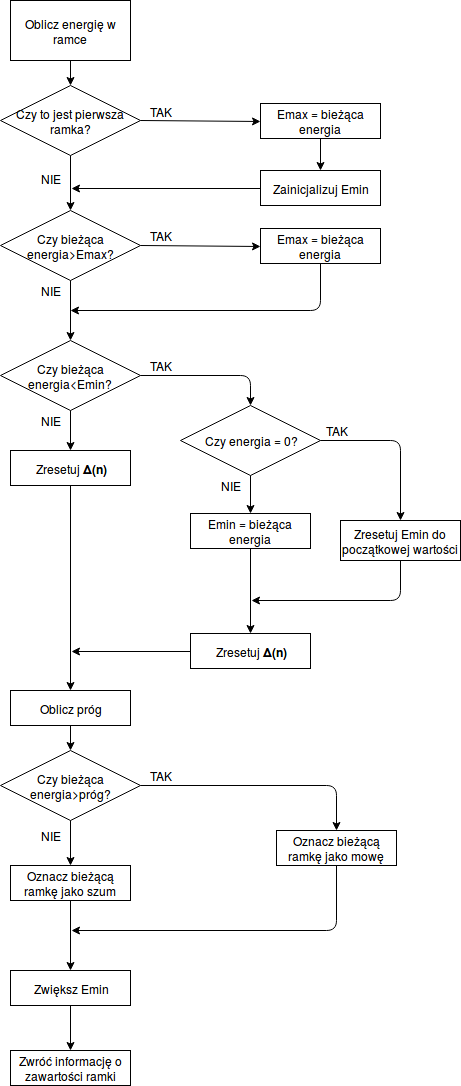
\includegraphics[scale=0.6]{EnergyBasedAlgorithmFlowchart.png}
	 	\caption{Schemat blokowy działania algorytmu bazującego na energii sygnału} 	
	 \end{center}
 \end{figure}
 
 Najbardziej powszechną metodą do obliczenia energii dla całego pasma  w sygnale mowy jest:
 
 
 \begin{equation}
	 E_{j} =\sum_{i=0}^{N}x^2(i)
 \end{equation}
 
 \hspace{8cm}gdzie: $E_{j}$ - energia j-tej ramki
 
 Jednak na potrzeby tego algorytmu energia ramki jest dodatkowo dzielona przez ilość próbek w ramce:
 
 \begin{equation}
 E_{n} = \frac{1}{N} E_{j} 
 \end{equation}
 
 \hspace{8cm}gdzie: N - ilość próbek w ramce
 
 
  \subsection{Początkowy próg detekcji \cite{energyAlgorithm}}
  ALgorytm detekcji startuje zwykle z początkowej wartości progu detekcji, a w trakcie analizy dolnych fragmentów wartość progu będzie się zmieniać, np. z powodu zmiany poziomu szumu.
  Przyjęto, że początkowe 100ms nagrania nie zawiera mowy, co wymaga uwzględnienia w trakcie rejestracji. Jest to podyktowane tym, że mówca potrzebuje czasu na rekację, nabranie powietrza, aktywację strun głosowych. Te 100ms są uznawane za przebieg pozbawiony sygnału mowy i ich średnia wartość obliczana jest zgodnie ze wzorem:
  
  \begin{equation}
  E_{r} =\frac{1}{V}\sum_{n=0}^{V}E_{n},
  \end{equation}
  
  gdzie: V - ilość ramek w początkowych 100ms przebiegu \vspace{5mm}
					 \hspace{1cm}$ E_{r}$ - początkowy próg detekcji
  
  
  \subsection{Próg detekcji zmieniający się dynamicznie w czasie \cite{energyAlgorithm}}
  Główną ideą tego algorytmu jest możliwośc obilczenia progu detekcji bez potrzeby korzystania z obszarów niezawierajacych mowy. Zamiast tego wykorzystywana jest minimalna oraz maksymalna energia sygnału mowy.   
  
  Innym popularnym sposobem na obliczenie energii sygnału mowy jest pierwiastek ze średniokwadratowej wartości energii (root mean square energy - RMSE), dany jako:
  
  \begin{equation}
	  E_{s} =\sqrt{E_n},
  \end{equation}
  
  Dynamiczny VAD jest oparty o obserwację, że estymata mocy sygnału mowy pokazuje wyraźne szczyty i doliny. Podczas gdy szczyty odpowiadają aktywności mowy, doliny mogą zostać wykorzystane do uzyskania estymaty mocy szumu.
  
  \subsection{Wyznaczanie progu \cite{energyAlgorithm}}
 Estymacja progu bazuje na poziomach energii $E_{min}$ oraz $E_{max}$ otrzymane z ciągu nadchodzących ramek. Te wartości są trzymane w pamięci i próg $\theta$ jest obliczany jako:
 
 \begin{equation}
	 \theta = k_{1}E_{max} + k_{2}E_{min}
 \end{equation}
 
  \hspace{8cm} gdzie $k_{1}$ i $k_{2}$ to współczynniki 
  
  \hspace{8cm}wykorzystane do interpolacji wartości
  
  \hspace{8cm} progu dla optymalnych wyników.\vspace{5mm} 
  
  Jeżeli energia bieżęcej ramki jest mniejsza niż wartość progu, ramka zostaje oznaczana jako niezawierająca mowy. 
  
  Jako, że mogą się pojawić pewne anomalie spowodowane zbyt niską energią, wprowadzono odpowiednią prewencję. Parametr $E_{min}$ jest nieznacznie zwiększany dla każdej ramki, zdefiniowane jako:
  
  \begin{equation}
  E_{min}(j) = E_{min}(j-1)\Delta(j)
  \end{equation}
  Parametr $\Delta$ dla każdej ramki jest zdefiniowany jako:
  
  \begin{equation}
  	\Delta(j) = \Delta(j-1) \cdot1.0001
  \end{equation}
  
  \subsection{Rozszerzenie algorytmu \cite{energyAlgorithm}}
  Możliwe jest przedstawienie równania na wyznaczenie dynamicznie zmieniającego się progu przy pomocy jednego parametru $\lambda$ (np. $\lambda$ = $k_{2}$).
  
  \begin{equation}
	  \theta = (1-\lambda)E_{max} + \lambda E_{min}
  \end{equation}
  
  \hspace{8cm}gdzie $\lambda$ to parametr skalujący , który 
  
  \hspace{8cm}kontroluje proces estymacji.
  
  Detektor mowy działa wiarygodnie, gdy $\lambda$ należy do przedziału [0.950, ..., 0.999]. Jednakże, wartości dla różnych typów sygnałów mogą nie być takie same i informacja a priori wciąż wymaga poprawnego ustalenia wartości $\lambda$. Równanie poniżej pokazuje jak sprawić, żeby współczynnik skalujący $\lambda$ był niezależny i odporny na zmieniające się warunki środowiska.
  
  \begin{equation}
  	\lambda = \frac{E_{max}-E_{min}}{E_{max}}
  \end{equation}
  
\newpage
 \section{Algorytm bazujący na obwiedni sygnału podzielonego na pasma z filtracją pojedynczych częstotliwości \cite{SFFAlgorithm}}
 
 \begin{figure}
 	\begin{center}
 		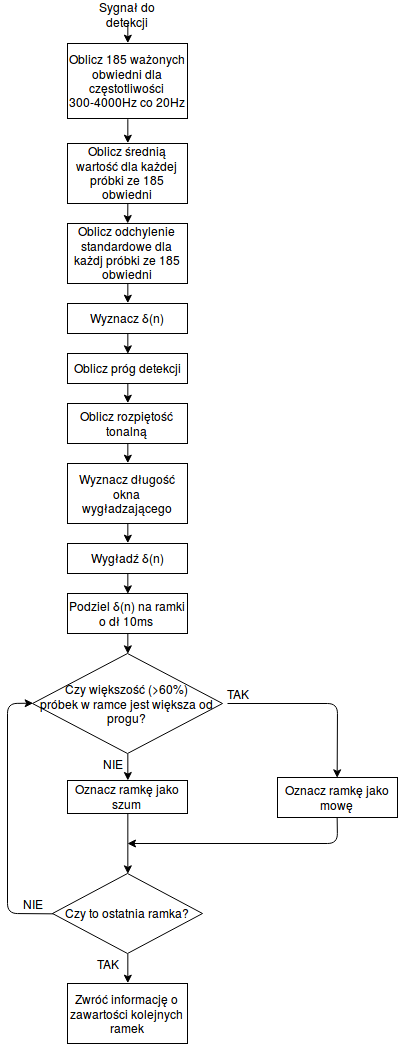
\includegraphics[scale=0.6]{SFFAlgorithm.png}
 		\caption{Schemat blokowy algorytmu SFF} 
 	\end{center}
 \end{figure}
 
 Algorytm ten, dla uproszczenia, w niniejszej pracy będzie często nazywany algorytmem SFF (Single Frequency Filtering). Bazuje on na obwiedniach dla sygnału podzielonego na 185 pasm - od 30Hz do 4000Hz, co 20Hz. Wybrany przedział częstotliwości pokrywa się z pasmem, w którym znajduje się mowa. Na Rysunku 3.2 przedstawiono schemat blokowy algorytmu SFF. Poniżej zostały przedstawione kolejne kroki potrzebne do policzenia 185 obwiedni i odpowiedniego przekształcenia ich w funkcję czasu, na której będzie można dokonać detekcji.
 
 
 \subsection{Obwiednie sygnału dla każdej częstotliwości}
 Sygnał mowy w zdyskretyzowanej dziedzinie czasu $s(n)$ jest różniczkowany i jest rozumiany jako $x(n) = s(n) - s(n-1)$. Częstotliwość próbkowania to $fs$. Sygnał $x(n)$ jest przemnażany przez zespoloną sinusoidę o danej znormalizowanej częstotliwości $\bar{\omega}_{k}$.  Wynik tej operacji w dziedzinie czasu jest dany jako: 
 
 \begin{equation}
	 x_{k}(n) = x(n)e^{j\bar{\omega}_{k}n},
 \end{equation}
 
 \hspace{8cm}gdzie $\bar{\omega}_{k} = \frac{2\pi\bar{f_{k}}}{f_{s}}$\vspace{5mm}
 
 Kiedy pomnożymy $x(n)$ przez $e^{j\bar{\omega}_{k}n}$, wynikowe widmo $x_{k}(n)$ będzie przesuniętym widmem $x(n)$. Czyli:
 
 \begin{equation}
	 X_{k}(\omega) = X(\omega - \bar{\omega}_{k}),
 \end{equation}
 
 gdzie $X_{k}(\omega)$ i $X(\omega)$ to odpowiednio widma  $x_{k}(n)$ i $x(n)$.\vspace{5mm}
 
 Sygnał $x_{k}(n)$ jest przepuszczany przez jednobiegunowy filtr, którego transmitancja jest dana jako:
 
 \begin{equation}
	 H(z) = \frac{1}{1+rz^{-1}}
 \end{equation}
 
 Jednobiegunowy filtr ma biegun na osi liczb rzeczywistych w odległości $r$ od początku układu współrzędnych. Lokalizacja pierwiastka jest w $z = -r$ na płaszczyśnie liczb zespolonych, co odpowiada połowie częstotliwości próbkowania, np. $fs/2$. Wyjście filtra $y_{k}(n)$ jest dane jako:
 
 \begin{equation}
	 y_{k}(n) = -r y_{k}(n-1)+x_{k}(n)
 \end{equation}
 
  Obwiednia sygnału $y_{k}(n)$ jest dana jako:
 
  \begin{equation}
  	e_{k}(n) = \sqrt{y_{kr}^2(n) + y_{ki}^2(n)},
  \end{equation} 
  
  \hspace{8cm}gdzie $y_kr(n)$ i $y_{ki}(n)$ są odpowiednio 
  
  \hspace{8cm}częścią rzeczywistą i urojoną $y_{k}(n)$.\vspace{5mm}
  
  Kiedy filtrowanie $x_{k}(n)$ będzie zrobione dla $\frac{f_{s}}{2}$, powyższa obwiednia $e_{k}(n)$ będzie odpowiadać obwiedni sygnału $x_{k}(n)$ przefiltrowanego w pożądanej częstotliwości
  
  \begin{equation}
  	f_{k} = \frac{f_{s}}{2} - \bar{f_{k}}
  \end{equation}
  
  Powyższa metoda estymowania obwiedni składowej dla częstotliwości $f_{k}$ jest określana jako podejście filtracji pojedynczych częstotliwości (Single Frequency Filtering). Wybór filtra z biegunem w $z=-r$ do estymacji obwiedni przefiltrownego sygnału wydaje się być bardziej odpowiedni, jako że obwiednie są obliczane w możliwie najwyższych częstotliwościach $(f_{s}/2)$. Ponadto, wybór filtru w stałej częstotliwości dla jakiejkolwiek pożądaniej częstotliwości $f_{k}$ zapobiega efektu przeskalowania w związku z różnymi wzmocnieniami filtrów w różnych częstotliwościach. Jeżeli biegun zostanie wybrany z obszaru na kole jednostkowym, np $z=r=-1$, może to skutkować niestabilnością wyjścia filtru. Stabilność filtru jest zapewniona dzięki przesunięciu bieguna nieco bardziej wewnątrz koła jednostkowego. Z tego powodu $r$ zostało dobrane jako 0.99.
  
  W tym badaniu obwiednia została obliczona dla każdych 20Hz w przedziale od 300Hz do 3000Hz jako funkcja w dziedzinie czasu. Wybrany został przedział częstotliwości 300-4000Hz, ponieważ pokrywa się z użytecznym pasmem wykorzystywanym przez mowę. Zatem mamy obwiednie dla 185 częstotliwości jako funkcja w dziedzinie czasu. Zasadniczo obwiednia może zostać obliczona dla każdej pożądanej częstotliwości.
  
  \subsection{Ważone składowe obwiedni sygnału mowy}
  Kiedy sygnał mowy ma bardzo dużą rozpiętość tonalną w dziedzinie częstotliwości, sygnał może mieć wysoką wartość mocy w niektórych częstotliwościach w każdej chwili czasowej. W tych częstotliwościach SNR będzie miał większą wartość, jako, że moc szumu będzie prawdopodobnie mniejsza w związku z większym rozkładem jednostajnym mocy. Nawet dla szumów z nierównomiernym rozkładem mocy, niższe korelacje próbek szumu skutkują w niższej rozpiętości tonalnej w rozpiętości mocy szumu przez częstotliwość, w porównaniu z sygnałem mowy. Zauważmy, że widmowa rozpiętość tonalna daje przejaw korelacji próbek w dziedzinie czasu. 
  
  Moc szumu tworzy funkcję cechy (podłogi) dla obwiedni dla każdej częstotliwości i poziom cechy zależy od rozkładu mocy szumu wobec częstotliwości. Podłoga jest bardziej jednorodna wobec czasu, jeżeli szum jest niemalże stacjonarny. Nawet jeżeli szum jest niestacjonarny, jest względnie stacjonarny ponad większymi przerwami w czasie niż sygnał mowy. W takich przypadkach, poziom cechy może zostać obliczony ponad długimi przerwami w dziedzinie czasu dla każdej częstotliwości, jeżeli jest to potrzebne.
  
  Żeby zrekompensować efekt szumu, wartość wagi dla każdej częstotliwości jest obliczana używając wartości funkcji cechy. Dla każdego wyrażenia, średnia $(\mu_{k})$ z 20 \% najmniejszych wartości, wartości obwiedni dla każdej częstotliwości $f_{k}$ jest wykorzystywana do obliczenia znormalizowanej wagi wartości $\omega_{k}$ dla danej częstotliwości. Wybór akurat 20\% wartości jest oparty o założenie, że jest przynajmniej 20\% ciszy w każdym wyrażeniu mowy. Znormalizowana waga wartości w każdej częstotiwości jest dana jako:
  
  \begin{equation}
  	\omega_{k} = \frac{\frac{1}{\mu_{k}}}{\sum_{l=1}^{N}	\frac{1}{\mu_{t}}},
  \end{equation}
  \hspace{10cm}gdzie N to liczba kanałów.
  
  Obwiednia $e_{k}(n)$ dla każdej częstotliwości $f_{k}$ jest przemnażana przez wartość wagi $w_{k}$ w celu zrekompensowania poziomu szumu w tej częstotiwości. Wynikowa obwiednia jest określana jako obwiednia z ważonymi komponentami. Zauważmy, że dzięki temu ważeniu obwiednia dla każdej częstotliwości jest dzielona przez estymatę cechy szumu $u_{k}$. 
  
  Do wszystkich sygnałów została dodana mała ilość białego szumu, żeby mieć pewność, że wartość funkcji cechy nie jest zerem. Dla obliczeń $w_{k}$, wartości w dodanych obszarach ciszy nie będą rozważane. 
  
  W każdej chwili czasu średnia ($\mu(n)$) kwadratu ważonych obwiedni obliczonych  wobec częstotliwości odpowiada w przybliżeniu energii sygnału w danej chwili. Oczekuje się, że $\mu(n)$ będzie wyższe dla mowy, niż dla szumu w obszarach, gdzie występuje sygnał mowy, ponieważ wartosci szumu są o obniżonej wadze. W każdej chwili czasu, odchylenie standardowe ($\sigma(n)$) kwadratu ważonych obwiedni rownież będzie względnie wyższe dla mowy niż dla szumu w obszarach mowy - związane jest to ze strukturą formantu. Dlatego $\sigma(n)+ \mu(n)$ jest na ogół wyższe w obszarach mowy i niższe w regionach pozbawionych mowy. Ponieważ oczekuje się, że rozpiętość szumu (po kompensacji) będzie niższa, zaobserwowano, że wartości $\sigma(n)-\mu(n)$ są zwykle niższe w obszarach pozbawionych mowy, w porównaniu do obszarów zawierających mowę. Pomnożenie $(sigma(n) + u(n))$ przez $(sigma(n)+ u(n))$ daje $(sigma^2(n) - u^2(n))$, co podkreśla kontrast pomiędzy obszarami zawierającymi mowę i tymi, które mowy nie zawierają.
  
  W związku z dużą rozpiętością tonalną wartości $(sigma^2(n) - u^2(n))$, ciężko jest zaobserwować obszary mowy z małymi wartościami  $(sigma^2(n) - u^2(n))$. Aby podkreślić kontrast pomiędzy obszarami mowy i obszarami niezawierającymi mowy, rozpiętość tonalna jest redukowana poprzez obliczenie
  
  \begin{equation}
	  \delta(n) =\sqrt[M]{|{(\sigma^2(n) - \mu^2(n))}|},
  \end{equation}
    \hspace{9cm}gdzie M zostało wybrane jako 64 \vspace{5mm}
   \begin{figure}
   	\begin{center}
    	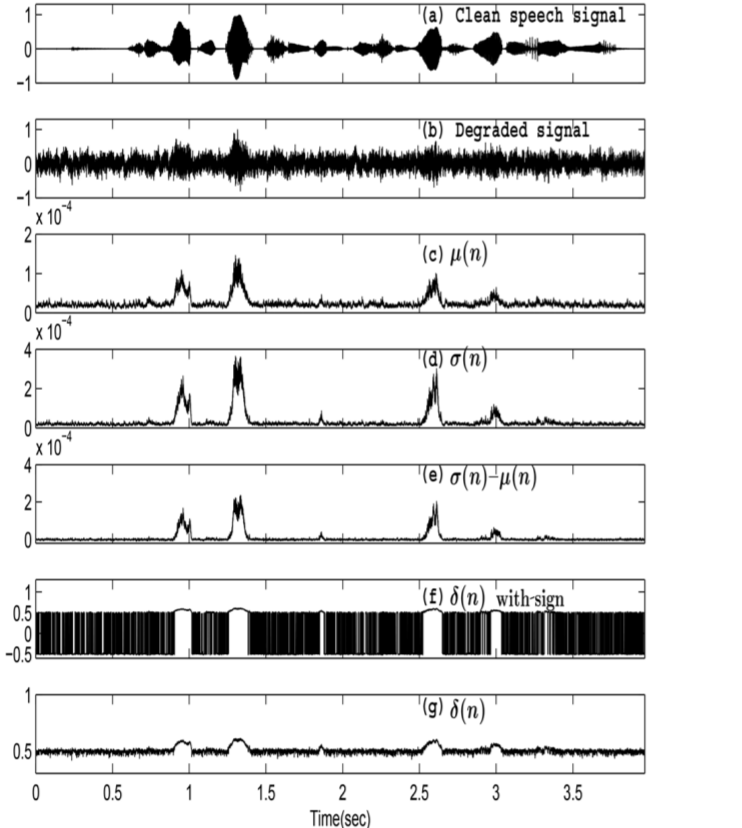
\includegraphics[scale=0.5]{SFFdelta.png}
   		\caption{Przykłady $\mu(n)$, $\sigma(n)$, $\sigma(n)- \mu(n)$, $\delta(n)$ ze znakiem, $\delta(n)$} 
   	\end{center}
   \end{figure}
   
    Wartość M nie jest decydująca. Każda wartość M z przedziału 32-256 wydaje się być dobra, aby zapewnić dobry kontrast pomiędzy obszarami zawierającymi mowę, a tymi, które mowy nie zawierają na wykresie $\delta(n)$. W obliczeniach $\delta(n)$ brana jest po uwagę tylko wartość bezwzględna wartości chwilowej $(\sigma^2(n) - \mu^2(n))$. Jeżeli znak wyrażenia $(\sigma^2(n) - \mu^2(n))$ jest przypisany do delta(n), wartości będą wahać się w okolicach zera w obszarach pozbawionych mowy dla większości typów szumów, ale krótki czas (20-40 msec) tymczasowych średnich wartości będzie mały i będzie się wahał, sprawiając, że cecha szumu będzie nierówna. To powoduje trudności w ustaleniu progu detekcji dla obszarów pozbawionych mowy. Wartości $\delta(n)$ będą miały wysoką średnią w obszarach pozbawionych mowy z małą średnią wariancją. Pomoże to w ustaleniu odpowiedniego progu do odizolowania obszarów pozbawionych mowy od tych, które mowę zawierają. Zakres $\delta(n)$ ze znakiem (Rys. 3.3(f)) jest inny niż wartości $\delta(n)$ (Rys. 3.3(g)). Mały tymczasowy obszar wartości $\delta(n)$ w obszarach niezawierających  mowy i jego średnia wartość pomagają w dobraniu pasującego progu. Wartości $\delta(n)$ w obszarach niezawierających mowy są podyktowane poziomem szumu. Zauważmy, że rozważając wartości  $\delta(n)$ bez znaku, tracimy trochę zalet w rozróżnialności obszarów niezawierających mowy, które maja zarówno dodatnie, jak i ujemne wartości - natomiast obszary zawierające mowę mają w większości dodatnie wartości. Wartości $\delta(n)$ z $M=64$ są wykorzystywane do dalszego przetwarzania do podejmowania decyzji. Warto zauważyć zmiany w przeskalowaniu na rys 3.3(f) i 3.3(g), aby zrozumieć istotę używania wartości bezwzględnej, np $\delta(n)$ bez znaku.
    
  \subsection{Logika podejmowania decyzji}
  Logika podejmowanej decyzji opiera się o $\delta(n)$ dla każdego wyrażenia poprzez wyprowadzenie najpierw progu detekcji z przyjętego z założenia obszaru zawierającego szum, a później zastosować ten próg na tymczasowo wygładzonych wartosciach $\delta(n)$. Rozmiar okna $l_{w}$ wykorzystany do wygładzenia $\delta(n)$ jest zaadoptowany w oparciu o estymatę rozpiętości tonalnej ($\rho$) energii zaszumionego sygnału dla każdego wyrażenia, zakładając, że jest przynajmniej 20\% obszarów zawierających ciszę w każdym wyrażeniu. Binarna decyzja odnośnie mowy i jej braku w każdej chwili czasowej, oznaczana odpowiednio jako 1 i 0, jest dalej wygładzana z wykorzystaniem okna adaptacyjnego, żeby dotrzeć do ostatecznej decyzji detekcji. Następujące 5 kroków opisuje implementację szczegółów w logice podejmowania decyzji:\vspace{5mm}
  
  1) Obliczenie progu ($\theta$):
  
  Należy obliczyć średnią $(\mu_{\theta})$ i wariancję $(\sigma_{\theta})$ dla 20\% najmniejszych wartości.
  
  Próg $\theta = \mu_{\theta} + 3\sigma_{\theta}$ jest używany we wszystkich przypadkach. Wartość $\theta$ zależy od analizownego wyrażenia. Zatem wartość progu, odpowiadająca wartości cechy z $\theta(n)$, jest adaptopwana do konkretnego wyrażenia w zależności od charakterystyki sygnału i szumu w tym wyrażeniu.\vspace{5mm}
  
  2) Wyznaczenie okna wygładzającego $l_{w}$:
  
  Energia $E_{m}$ sygnału $x(n)$ jest obliczana dla ramki 300msec z przesunieciem 10msec, gdzie $m$ to numer ramki. Rozpiętość tonalna $(\rho)$ sygnału jest obliczana jako:
  
  \begin{equation}
	  \rho = 10\log_{10}\frac{max_m(Em)}{min_m(Em)}).
  \end{equation}
  
  
  Parametr opisujący długość okna $l_{w}$ do wygładzenia sygnału jest uzyskiwany z rozpiętości tonalnej $(\rho)$ sygnału.  Wartości $\rho$ różnią się dla różnych szumów przy tym samym SNR, ponieważ charakterystyki szumów się różnią. Wskaźnik SNR dla mowy z dystansu zależy od warunków środowiskowych oraz od odległości, z jakiej mówca mówi do mikrofonu.  Zaobserwowano, że wartości ro dla mowy z odległości są rozciągnięte w porównaniu z wartościami ro dla różnych szumów. Jest to głównie spowodowane efektem echa. Rozkład wartości ro zależy również od odległości mówcy od mikrofonu. Wartość $\rho$ dla każdego wyrażenia jest wykorzystywana do określenia wartości niektórych parametrów do dalszego przetwarzania $\delta(n)$ i do otrzymania decyzji o klasyfikacji. W przypadkach, gdzie $\delta(n)$ reprezentuje charakterystyka dyskryminacyjna przedstawiająca zarówno mowę, jak i jej brak, odpowiadające wartości $\rho$ są wysokie, jak zaobserwowano w przypadku szumów volvo, lamparta i karabinu maszynowego. W takich przypadkach używane są małe wartości parametru $l_{w}$ okna wygładzającego. Następujące wartości $l_{w}$ zostały wybrane na drodze przeprowadzonych doświadczeń z sygnałem mowy zaszumionym przez różne typy szumów z różnymi poziomami SNR:
  
  $$l_{w} = 400msec,\hspace{3mm}dla\hspace{2mm} \rho<30 $$
  
  $$l_{w} = 300msec,\hspace{3mm}dla\hspace{2mm} 30\leq\rho<40 $$
  
  $$l_{w} = 200msec,\hspace{3mm}dla\hspace{2mm} \rho>40.$$\vspace{5mm}
  
  3) Logika podejmowania decyzji w każdej chwili czasowej:
  
  Wartości $\delta(n)$ są uśredniane przez okno o rozmiarze $l_{w}$, aby otrzymać uśrednione wartości $\bar{\delta}(n)$ w każdej próbce o indeksie n. Decyzja jest podejmowana według następujących zależności:
  
  $$d(n) = 1,\hspace{3mm}dla\hspace{2mm}\bar{\delta}(n)>\theta$$
  
  $$d(n) = 0,\hspace{3mm}dla\hspace{2mm}\bar{\delta}(n)\leq\theta.$$\vspace{5mm}
  
  4) Wygładzenie decyzji na poziomie próbek:
  
  Decyzja $d(n)$ dla każdej próbki jest okienkowana o rozmiarach okienek 300msec, 400msec, 600msec, dla, odpowiednio, $\rho<30$, $30\leq\rho<40$, $\rho>40$ . Załóżmy, że $\eta$ jest progiem (w procentach) w zależności od wartości $d(n)$, które dają 1 w okienku. Jeżeli wartość procentowa wartości $d(n)$, które wynoszą 1 w okienku, jest wyższa niż wartość $\eta$, wtedy ostateczna decyzja $d_f(n)$ jest ustawiana na 1 w chwili czasowej $n$, w przeciwnym wypadku - 0. Wartość przypisana dla $\eta$ to 60\%.\vspace{5mm}
  
  5) Decyzja na poziomie ramek:
  
  Decyzja w metodzie AMR jest podejmowana dla każdej ramki, co 10msec. W celu porównania zaproponowanej metody z metodą AMR, decyzja $d_{f}(n)$ jest konwertowana na 10msec ramkę w oparciu o podjętą decyzję. Dla każdej 10msec, nienakładającej się ramki, jeżeli przeważająca ilość decyzji $d_{f}(n)$ wynosi 1, to cała ramka jest oznaczana jako zawierająca mowę, w przeciwnym wypadku jest oznaczana jako niezawierająca mowy. Informacje dotyczące sygnałów mowy pozyskane z empirycznie, są rownież otrzymywane z każdej 10msec ramki.
  
  
 \newpage
 
\section{Zmieniony algorytm Single Frequency Filtering (SFF2)}
W dalszej części pracy, jako, że ten algorytm bazuje na założeniach SFF, będzie nazywany algorytmem SFF2.
W celu zmniejszenia złożoności obliczeniowej oraz zwiększenia dokładności detekcji, zostały zaproponowane pewne zmiany w algorytmie SFF:\vspace{5mm}

1) Zmiana w sposobie obliczania obwiedni sygnału.\vspace{5mm}

2) Algorytm SFF zakłada obliczenie 185 obwiedni począwszy od 300Hz do 4000Hz co 20Hz. Doświadczalnie sprawdzono, że wystarczające jest obliczenie co czwartej obwiedni zaczynając od 300Hz, oraz zaczynając od 340Hz, co 20Hz każda. Zatem, zamiast 185 obwiedni, liczonych jest jedynie 92. \vspace{5mm}

3) Zmiana w sposobie liczenia progu detekcji. Liczone jest 15\% z najmniejszych wartości. Tworzony jest również histogram dla $\delta(n)$, na podstawie którego zostaje wyliczonych 15\% najmniejszych wartości. Znacząco zwiększa to szybkość wykonywanych obliczeń.\vspace{5mm}


\chapter{Wyniki badań}
\section{Sposób oceny}
	Do przeprowadzenia badań zostały wybrane 2 sygnały (głos damski oraz głos męski) zawierające pojedyncze słowa oraz 2 sygnały zawierające ciągi słów. Pierwszy etap badań założył manualne wybranie próbek zawierających początki oraz końce wypowiedzi, rozważony został przypadek, gdy mowa rozpoczyna się w momencie generowania słyszalnych dźwięków przez mówcę.
	Następnie te same sygnały zostały zbadane przez 3 algorytmy detekcji, które również wybrały numery próbek, które miały reprezentować początki i końce mowy. Dla każdego pomiaru wykonano 10 prób i ostateczne wartości poddane badaniom są średnią wartością z tych prób. Jako główne kryterium oceny przyjęto odległość zdetekowanego rozpoczęcia lub końca aktywności od rozpoczęcia lub końca aktywności ze wzorca (w próbkach). 
		
 Następnie została policzona wartość bezwzględna próbki wybranej manualnie oraz próbki wybranej przez algorytm. Często pojawia się sytuacja, że któryś z algorytmów podjął decyzję o większej lub mniejszej ilosci początkow lub końców mowy. W związku z tym dodano nowe kryterium, jakim jest ilość detekcji. Za każdy nadprogramowy początek lub koniec doliczana jest pewna wartość, którą można potraktować jako karę za błąd. Ponadto, jeżeli któryś z obszarów zaznaczonych we wzorcu jako obszar zawierający mowę nie został odpowiednio zdetekowany, doliczana jest dodatkowa kara o wartości 50. Przedstawione w tabelach wartości $Wynik$ zostały obliczone zgodnie ze wzorem 
 
 \begin{equation}
 	Wynik = |d_{\textrm{wzór}} - d_{alg}|*kara + \sum_{i=1}^{j}| x_{\textrm{wzór}}(i)-x_{alg}(i) |,
 \end{equation}
 
 gdzie $d_{\textrm{wzór}}$ to sumaryczna ilość początków i końców detekcji we wzorze, $d_{alg}$ to sumaryczna ilość początków i końców detekcji wybranego algorytmu, $kara$ to stała wartość, w tym przypadku ustawiona na $50$, $i$ to numer kolejnej detekcji, $j$ to ilość wszystkich detekcji, $x_{\textrm{wzór}}(i)$ to nr próbki wybranej manualnie, a $x_{alg}(i)$, to numer próbki wybranej przez algorytm.
 
  Wyniki dla poszczególnych algorytmów, w dwóch rozważanych przypadkach zostały przedstawione w tabeli poniżej. Oznaczenia algorytmów: En - algorytm bazujący na energii sygnału, SFF - algorytm bazujący na obwiedni sygnału, SFF2 - zmieniony algorytm SFF.

\begin{figure}
\section{Wyniki dla pojedynczych słów}
	Na rysunku 5.1 przedstawiono przebieg czasowy wyrazu \emph{kabanos}, głos damski, a na rysunku 5.5 przebieg czasowy wyrazu \emph{zapamiętaj}, głos męski, które zostaną poddane detekcji przez algorytmy, które zostały zaprezentowane w poprzednich rozdziałach. Na rysunkach 5.1 oraz 5.5 detekcja została ustawiona manualnie, jako punkt odniesienia dla innych algorytmów.
	Kolejne rysunki zawierają wyniki detekcji.
\end{figure}

	\begin{figure}
		\begin{center}
			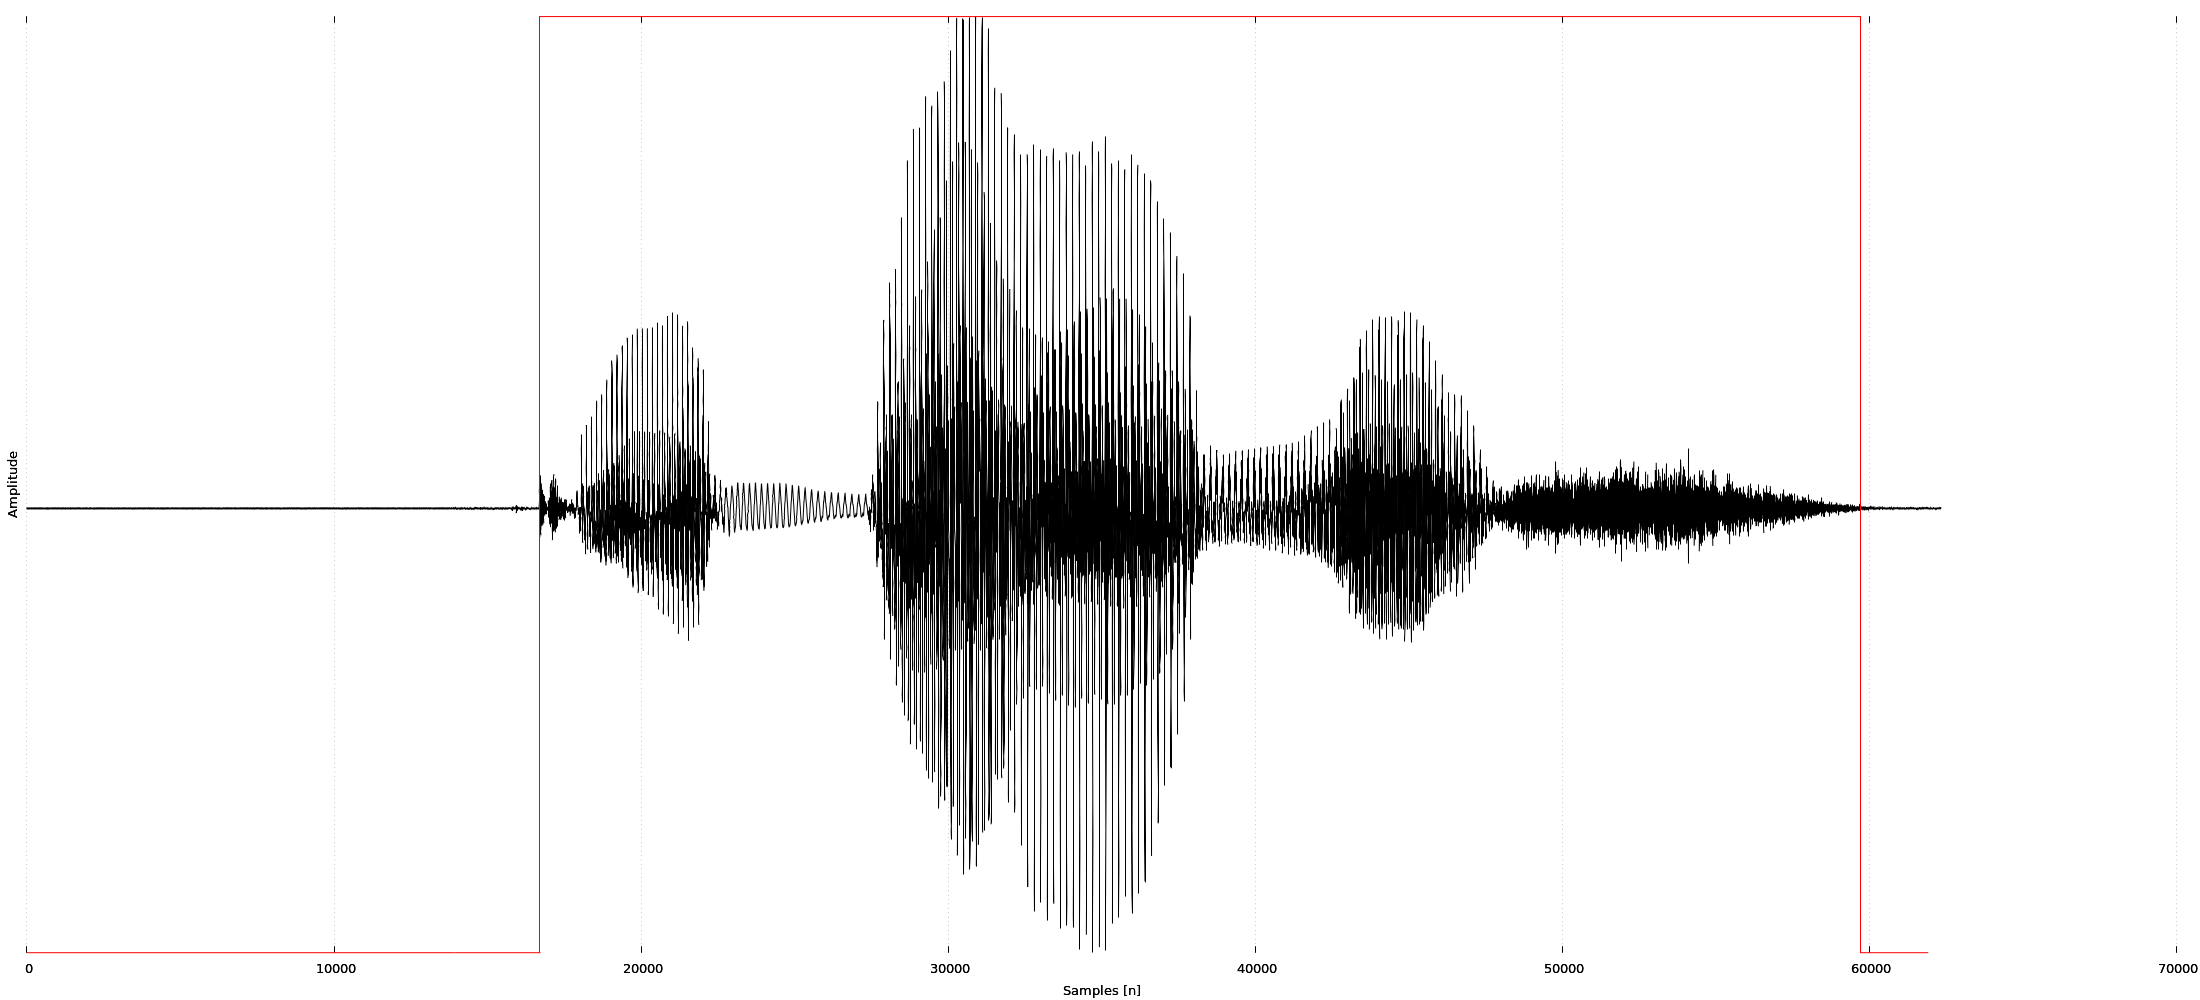
\includegraphics[scale=0.2]{kabanos.png}
			\caption{Przebieg czasowy słowa \emph{kabanos} i jego wzorcowa detekcja}\vspace{5mm}
		\end{center}
	\end{figure}
	\begin{figure}
		 \begin{center}
			 	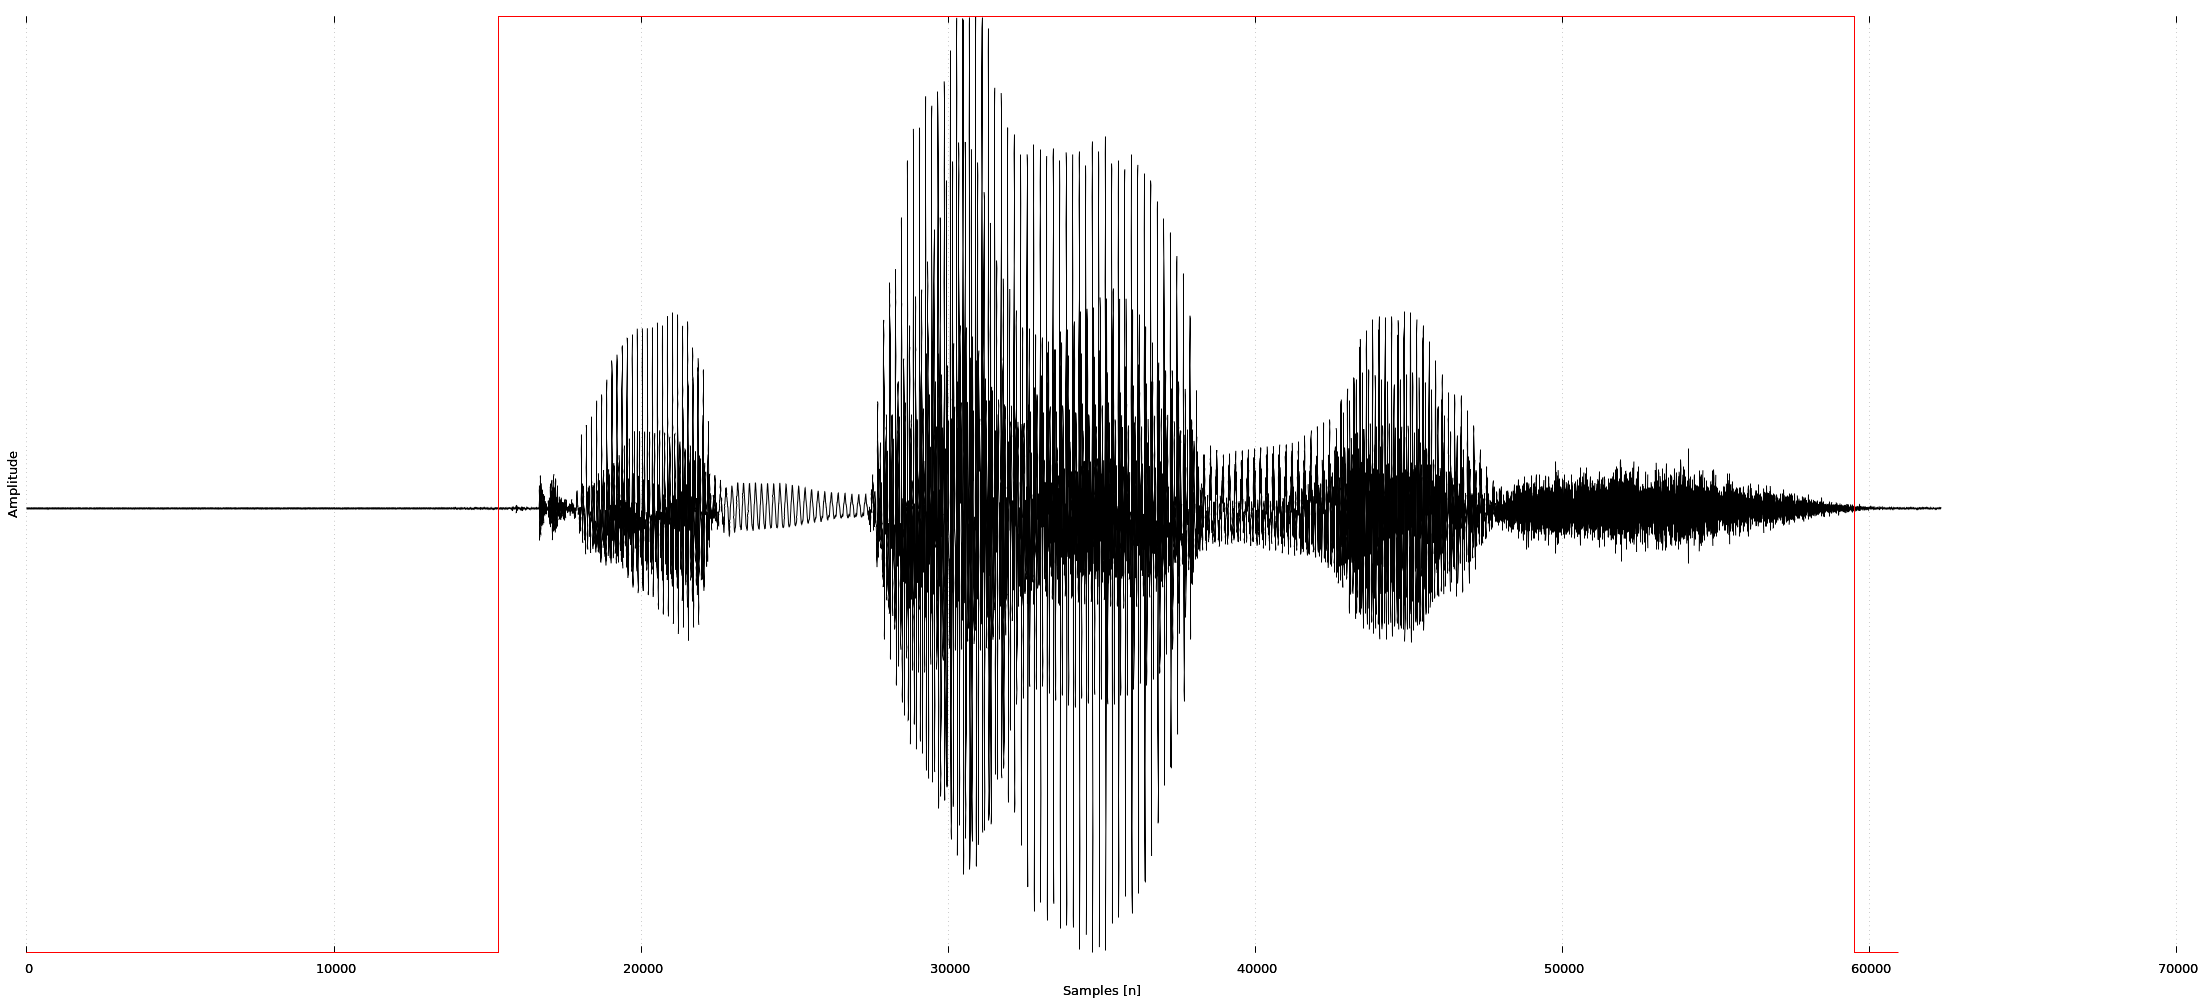
\includegraphics[scale=0.2]{kabanosEnergy.png}
			 	\caption{Wynik detekcji algorytmu bazującego na energii sygnału}\vspace{5mm}
			 	
			 	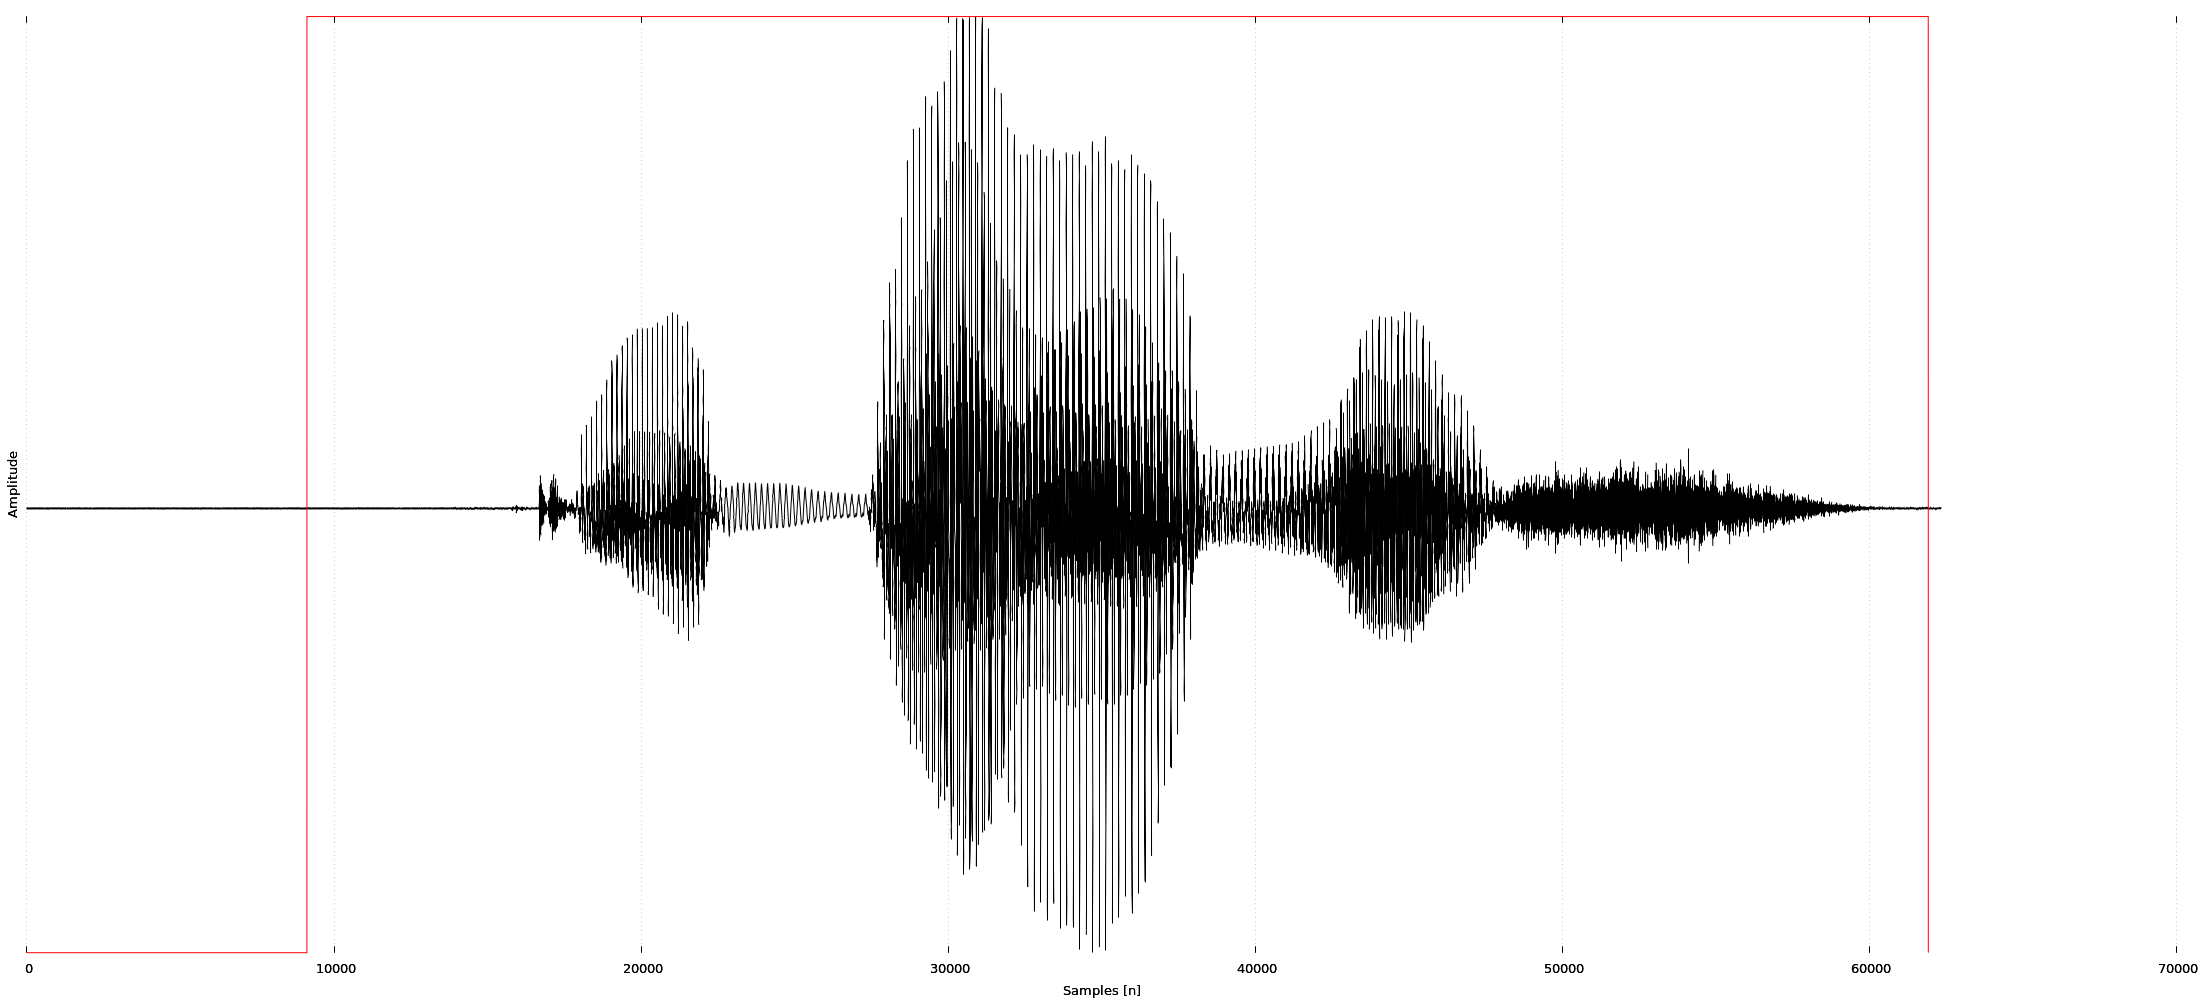
\includegraphics[scale=0.2]{kabanosSFFArticle.png}
			 	\caption{Wynik detekcji algorytmu SFF}\vspace{5mm}
			 	
			 	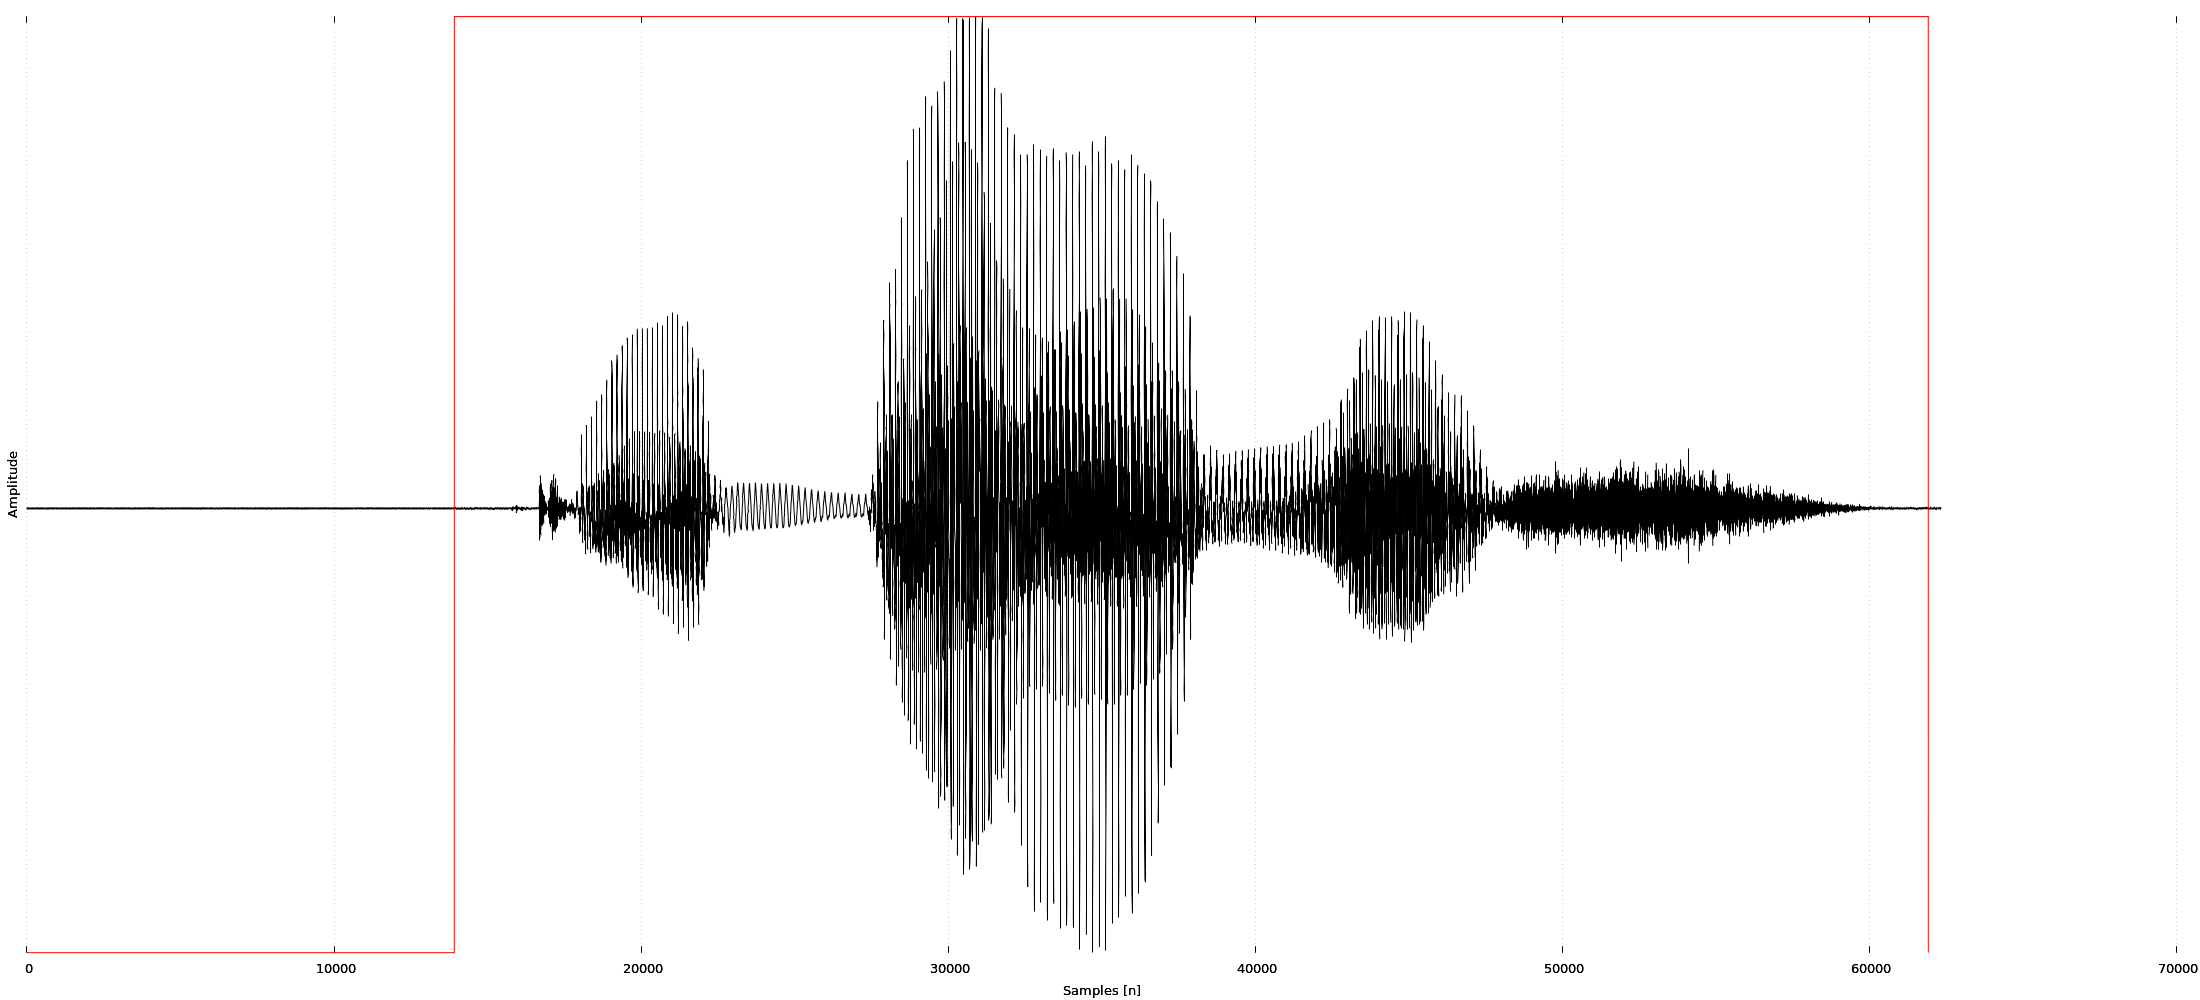
\includegraphics[scale=0.2]{kabanosSFFChanged.png}
			 	\caption{Wynik detekcji algorytmu SFF2}\vspace{5mm}
		\end{center}
	\end{figure}
	
	
	\begin{figure}
	 	\begin{center}
	 		$\begin{array}{ | c | c | c | c | c | }
	 			\hline
	 			& \textrm{Wzorzec}&\textrm{En[nr probki]} & \textrm{SFF[nr probki]} & \textrm{SFF2[nr probki]} \\ \hline
	 			\textrm{Początek} & 6705 & 15360 & 9121 & 13921  \\ \hline
	 			\textrm{Koniec} & 59712 & 60000 & 61920 & 61920  \\ \hline
	 			\textrm{SUMA RÓŻNIC} & 0 & 1633 & 9792 & 4992    \\ \hline
	 		\end{array}$
	 		\caption{Wyniki działania algorytmów na słowie \emph{kabanos}}\vspace{5mm}
	 	\end{center}
	 	
	 	\begin{center}
	 		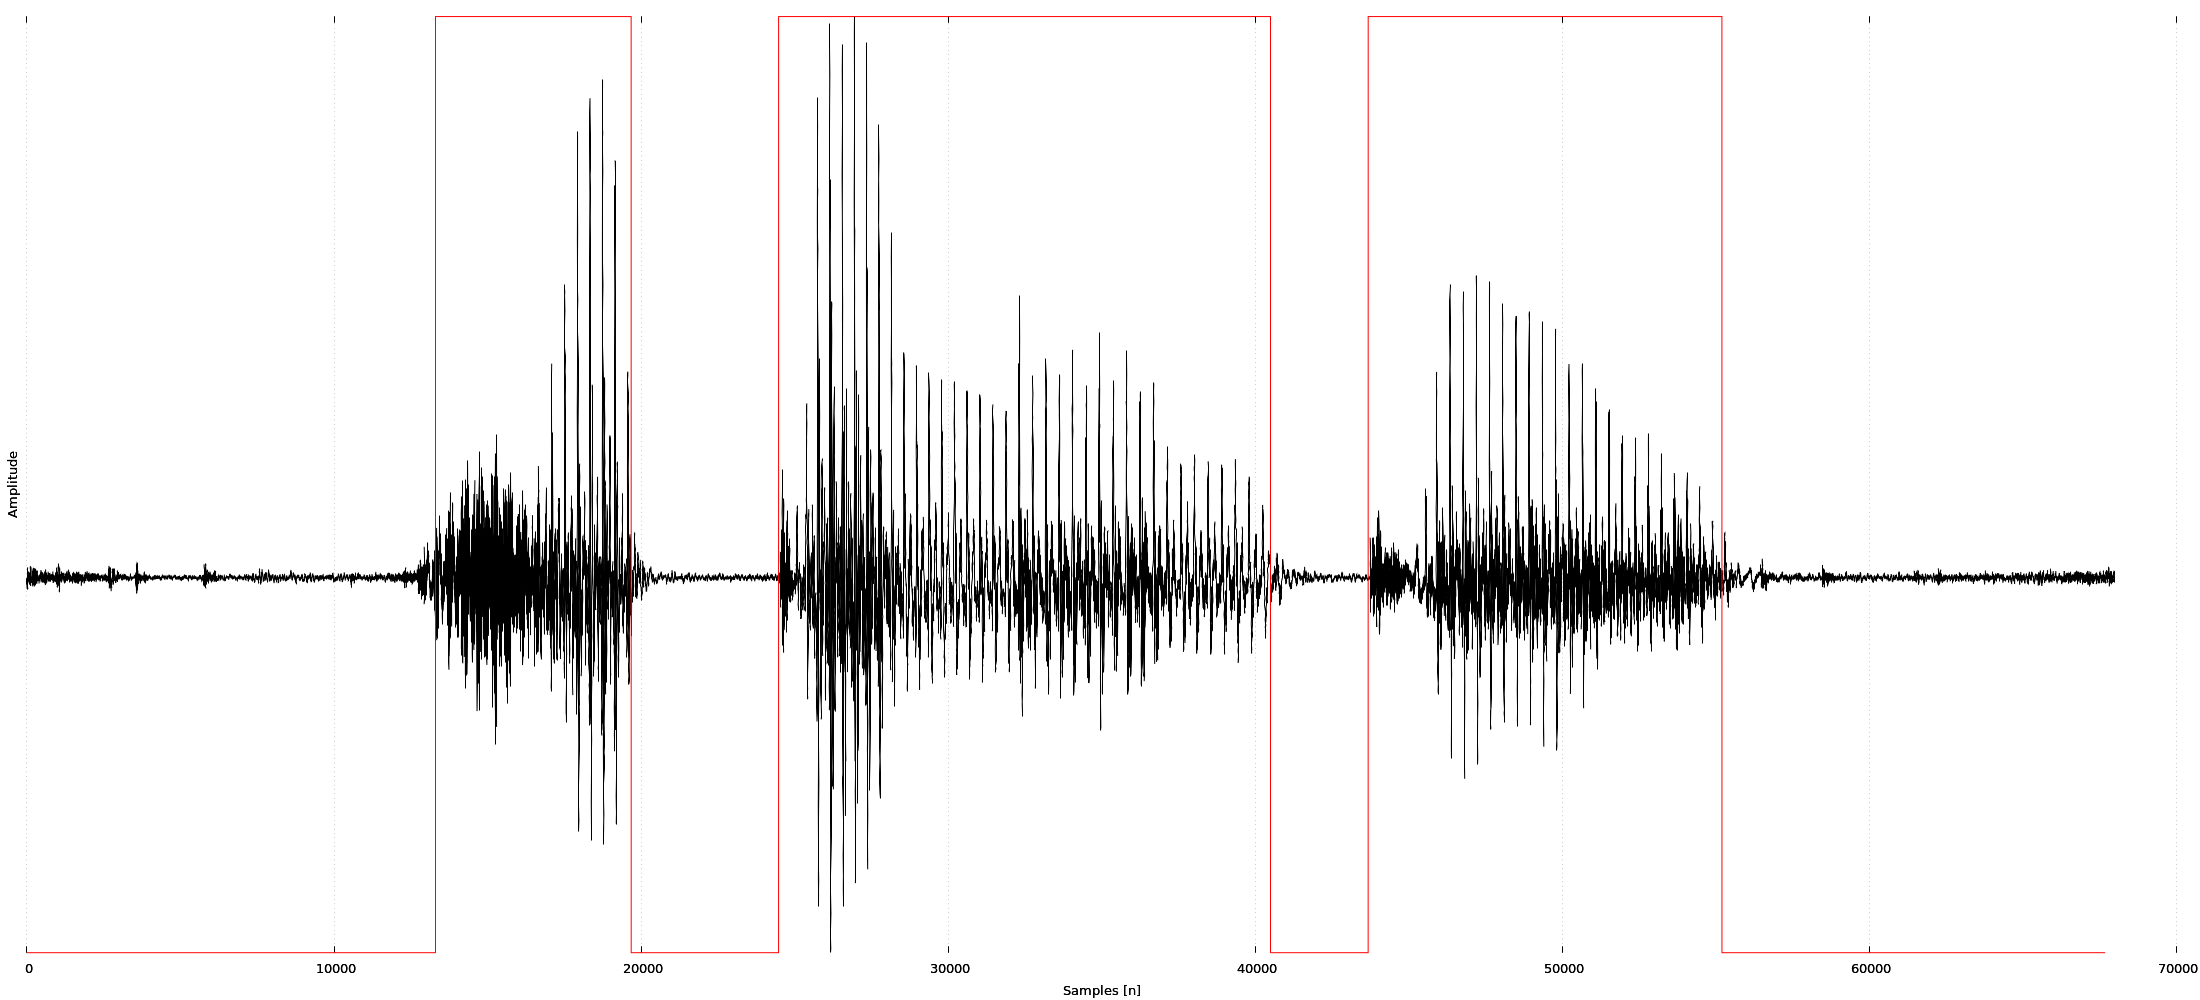
\includegraphics[scale=0.2]{zapamietaj.png}
	 		\caption{Przebieg czasowy słowa \emph{zapamiętaj} i jego wzorcowa detekcja}\vspace{5mm}
	 	\end{center}
	\end{figure}
 
	 
	 \begin{figure}
	 	\begin{center}
	 		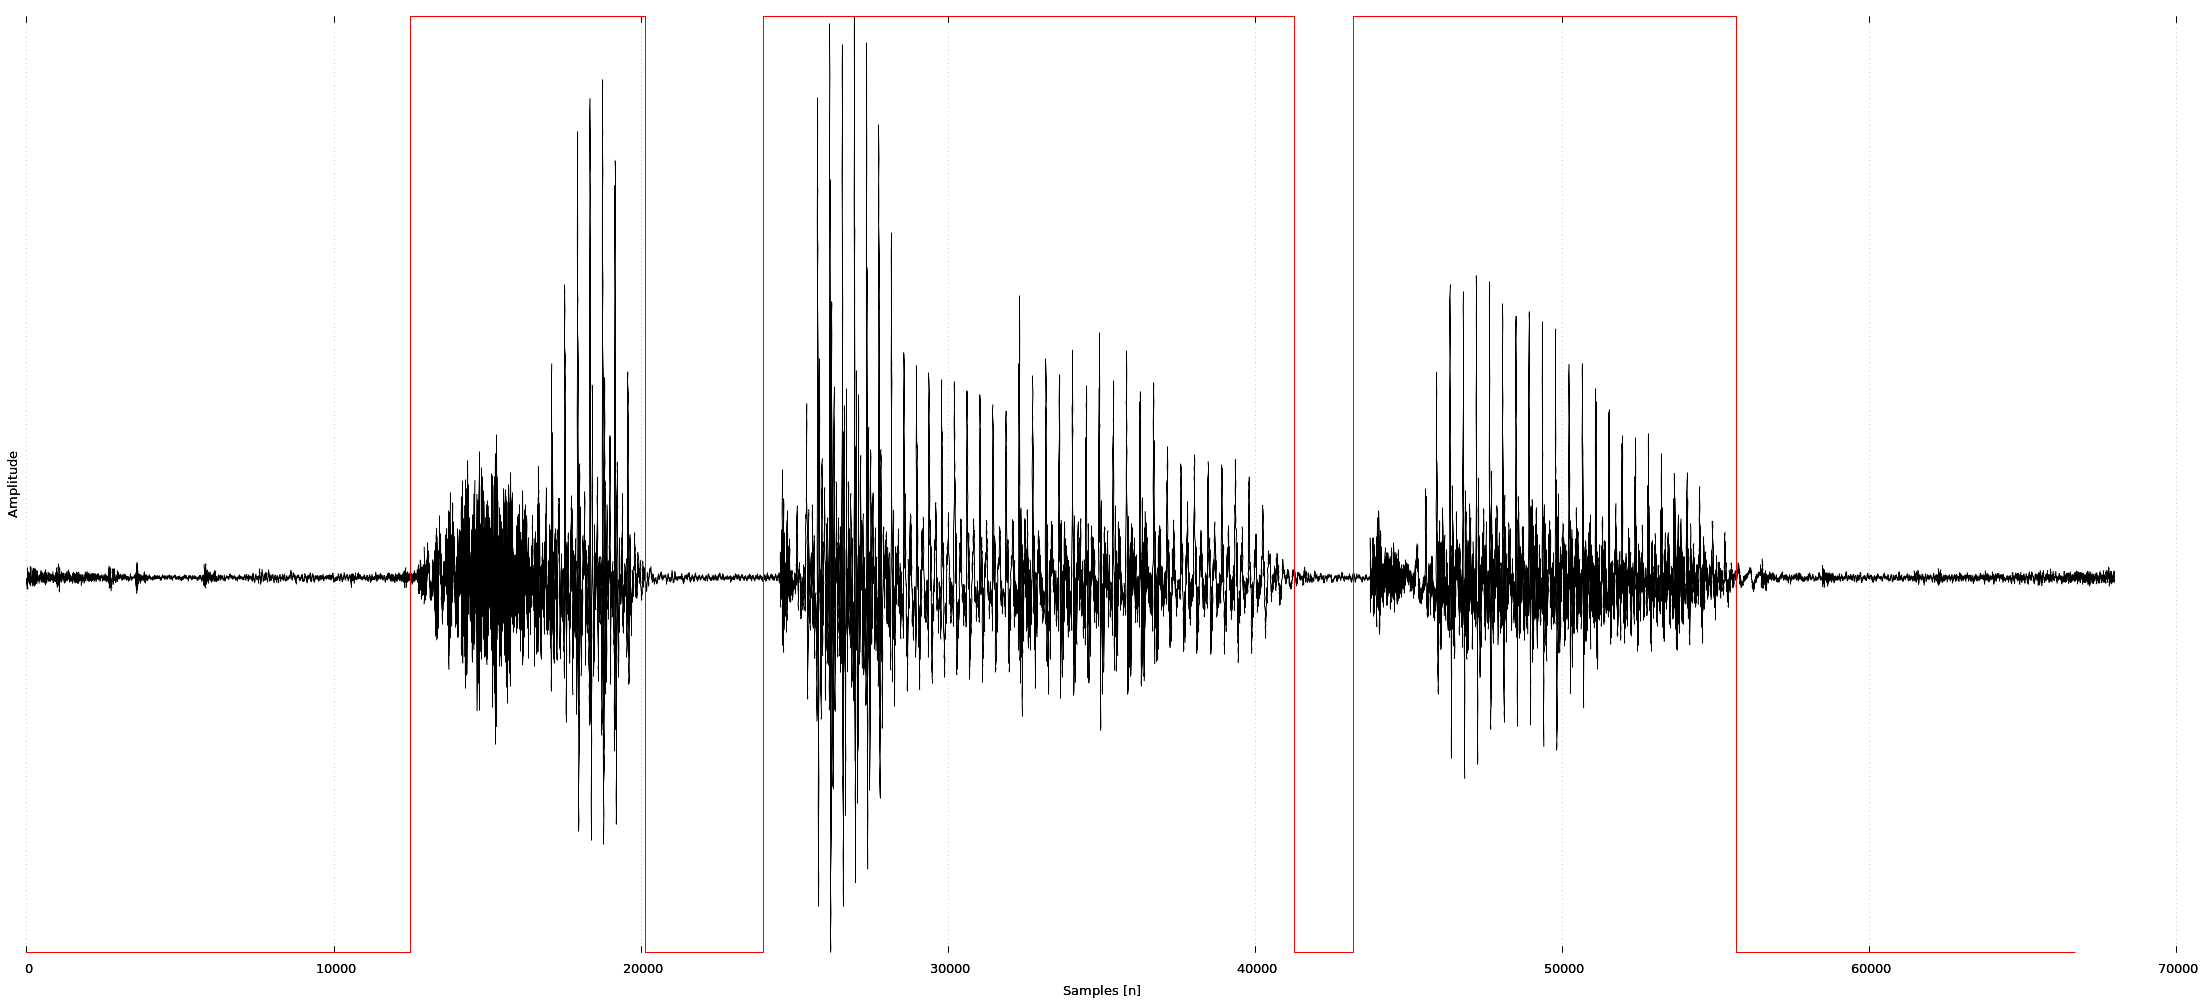
\includegraphics[scale=0.2]{zapamietajEnergy.png}
	 		\caption{Wynik detekcji algorytmu bazującego na energii sygnału}\vspace{5mm}
	 		
	 		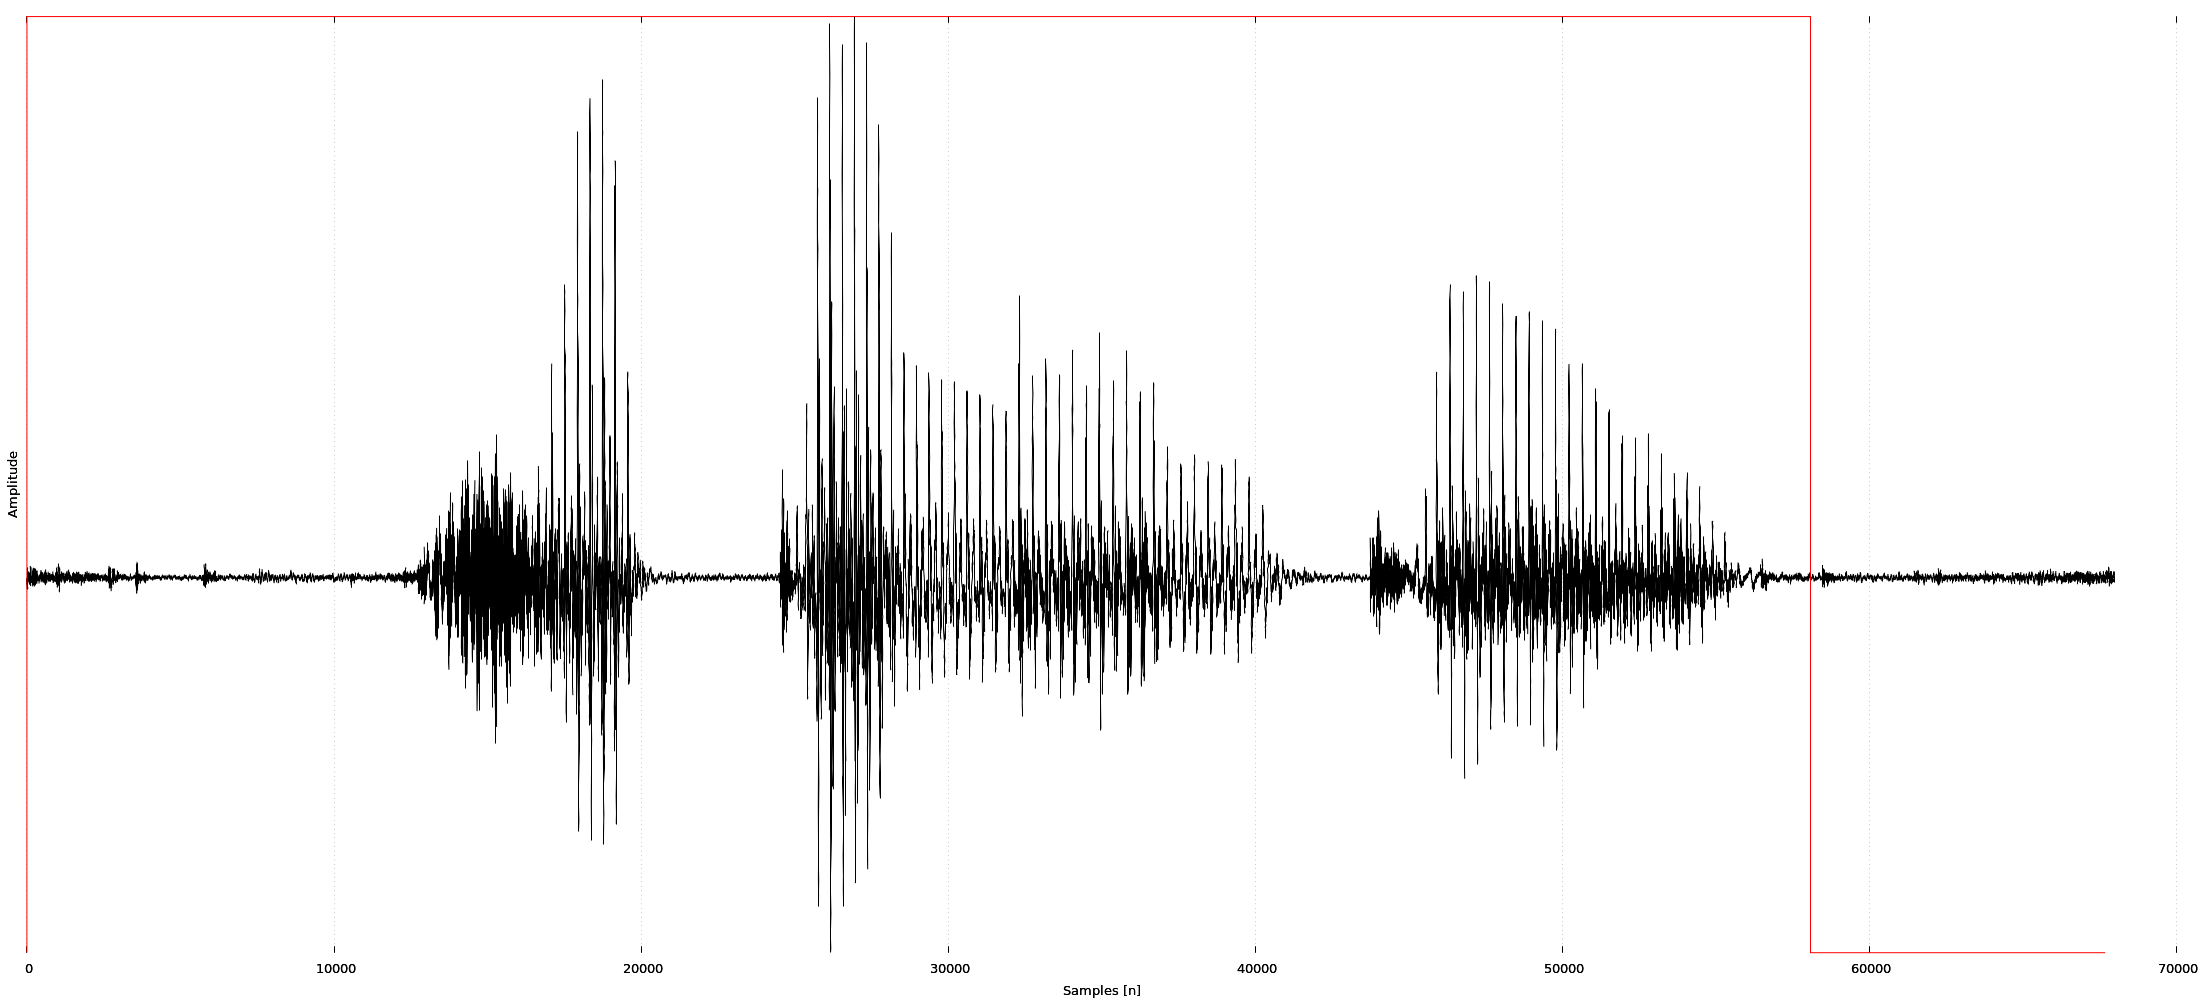
\includegraphics[scale=0.2]{zapamietajSFFArticle.png}
	 		\caption{Wynik detekcji algorytmu SFF}\vspace{5mm}
	 		
	 		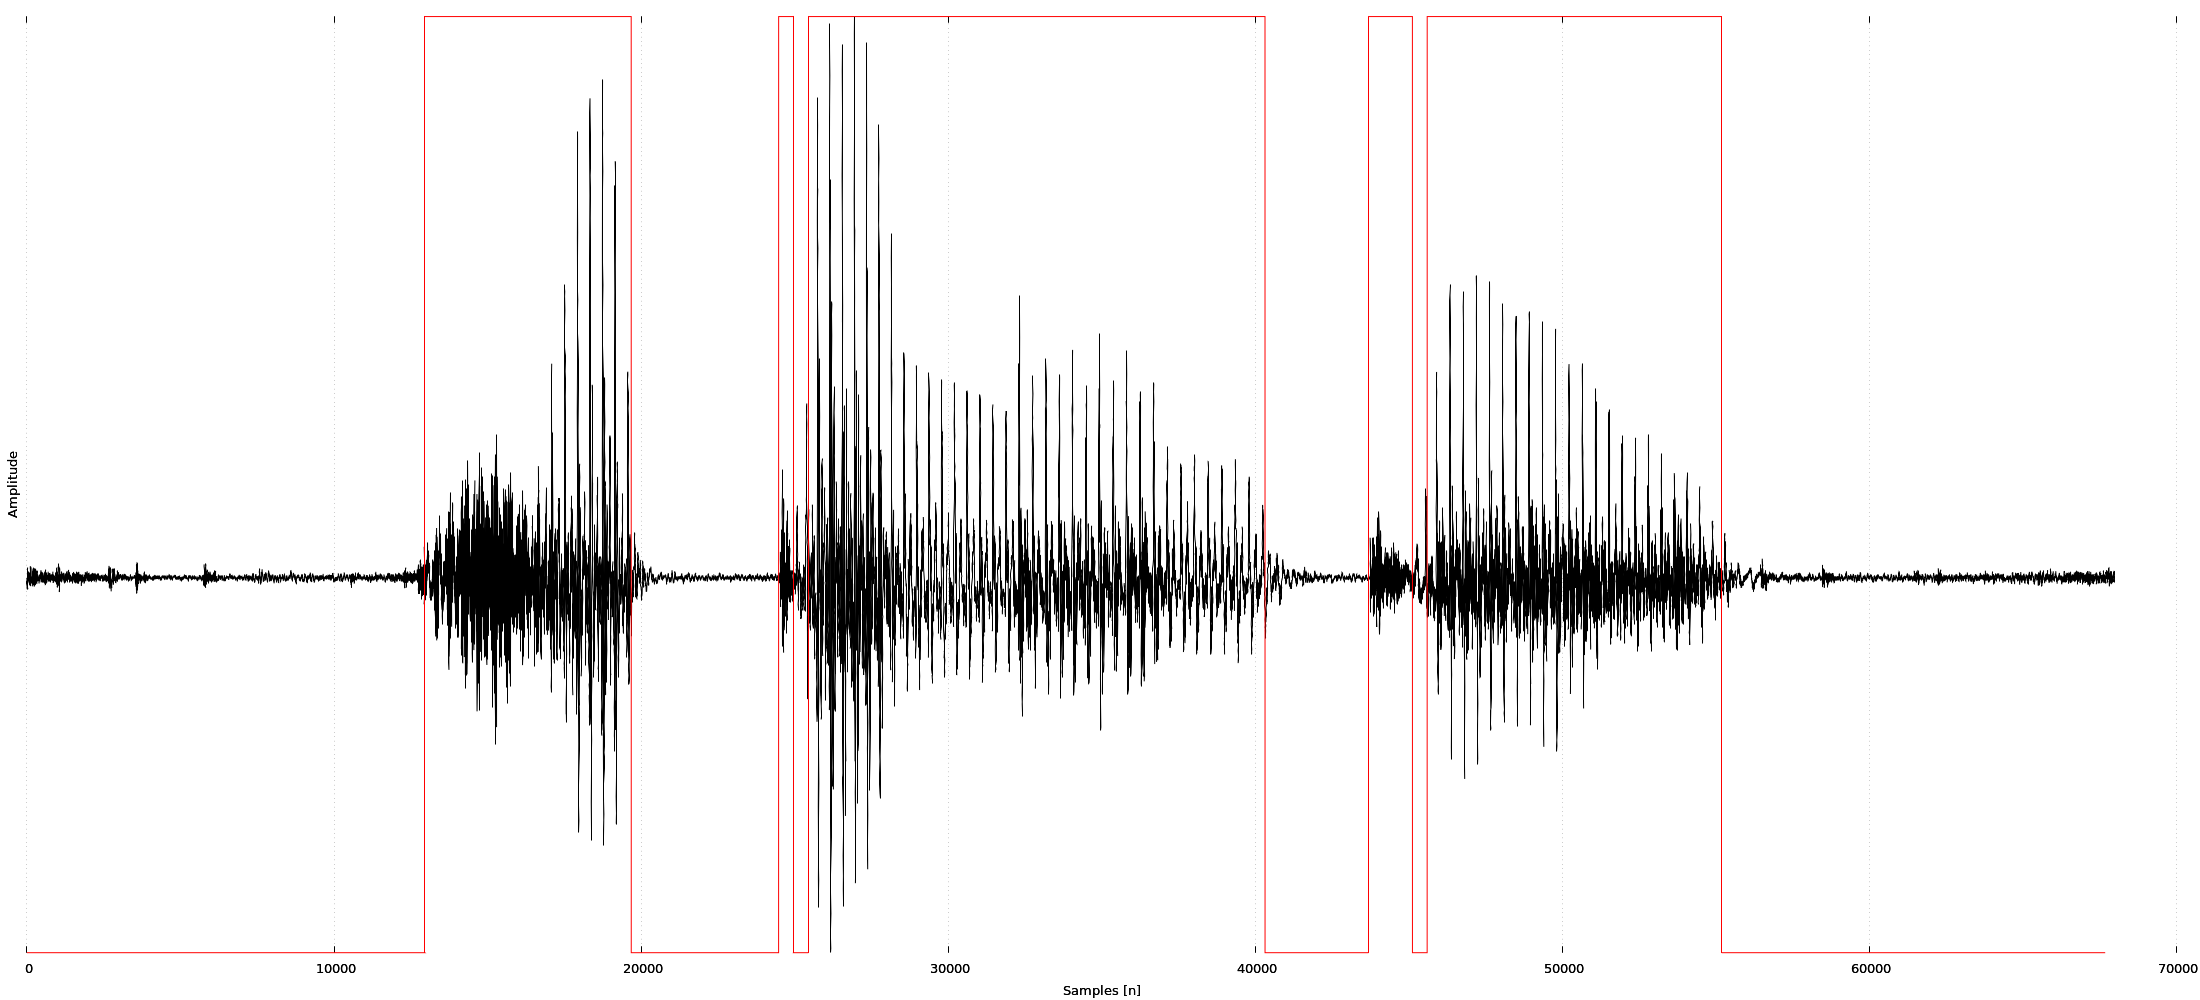
\includegraphics[scale=0.2]{zapamietajSFFChanged.png}
	 		\caption{Wynik detekcji algorytmu SFF2}\vspace{5mm}
	 	\end{center}
	 \end{figure}
	 
	 \begin{figure}
	 	\begin{center}
	 		$\begin{array}{ | c | c | c | c | c | }
	 		\hline
	 		& Wzorzec & En[nr probki] & SFF[nr probki] & SFF2[nr probki] \\ \hline
	 		 & 13296 & 12480 & 2 & 12961 \\ \hline
	 		 & 19680 & 20160 & & 19681   \\ \hline
	 		 & 24480 & 24000 & & 24481    \\ \hline
	 		 & 40512 & 41280 & & 40321  \\ \hline
	 		 & 43680 & 43200 & & 43681   \\ \hline
	 		 & 55200 & 55680 & 58081 & 55201 \\ \hline
	 		\textrm{SUMA RÓŻNIC} & 0 & 3504 & 16175 & 530 \\ \hline
	 		\textrm{Ilość detekcji} & 6 & 6 & 2 & 10 \\ \hline
	 		\textrm{Wynik} & 0 & 3504 & 16375 & 730 \\ \hline
	 		\end{array}
	 		$
	 		\caption{Wyniki działania algorytmów na słowie \emph{zapamiętaj}}
	 	\end{center}
	 	
	 \end{figure}
	 
	 
\begin{figure}

\section{Wyniki dla ciągów słów}
	Podobnie jak w poprzednim przypadku, na rysunku 5.11 przedstawiono przebieg czasowy kolejnych słów: \emph{grzech, poprzedni, móżdżek, widzenie, dzwoń, proszek, zapamiętaj, dziwak, radzić, fifka, szeregi, gorzki, kiedyś, ogród}, głos damski, natomiast na rysunku 5.16 pokazano wzorcową detekcję przebiegu czasowego kolejnych słów: \emph{poczta, buczek, turniej, radża, wyczyść, sęk, sześć, leżeć, dzień, fajka, wzrok, łazik, zlepek, poziomo},głos męski. Zaznaczono na nich oczekiwaną (wzorcową) detekcję algorytmów.
	Kolejne rysunki zawierają wyniki detekcji algorytmów.\\
	
	
\end{figure}


\begin{sidewaysfigure}
	\begin{center}
		\resizebox{\width}{2cm}{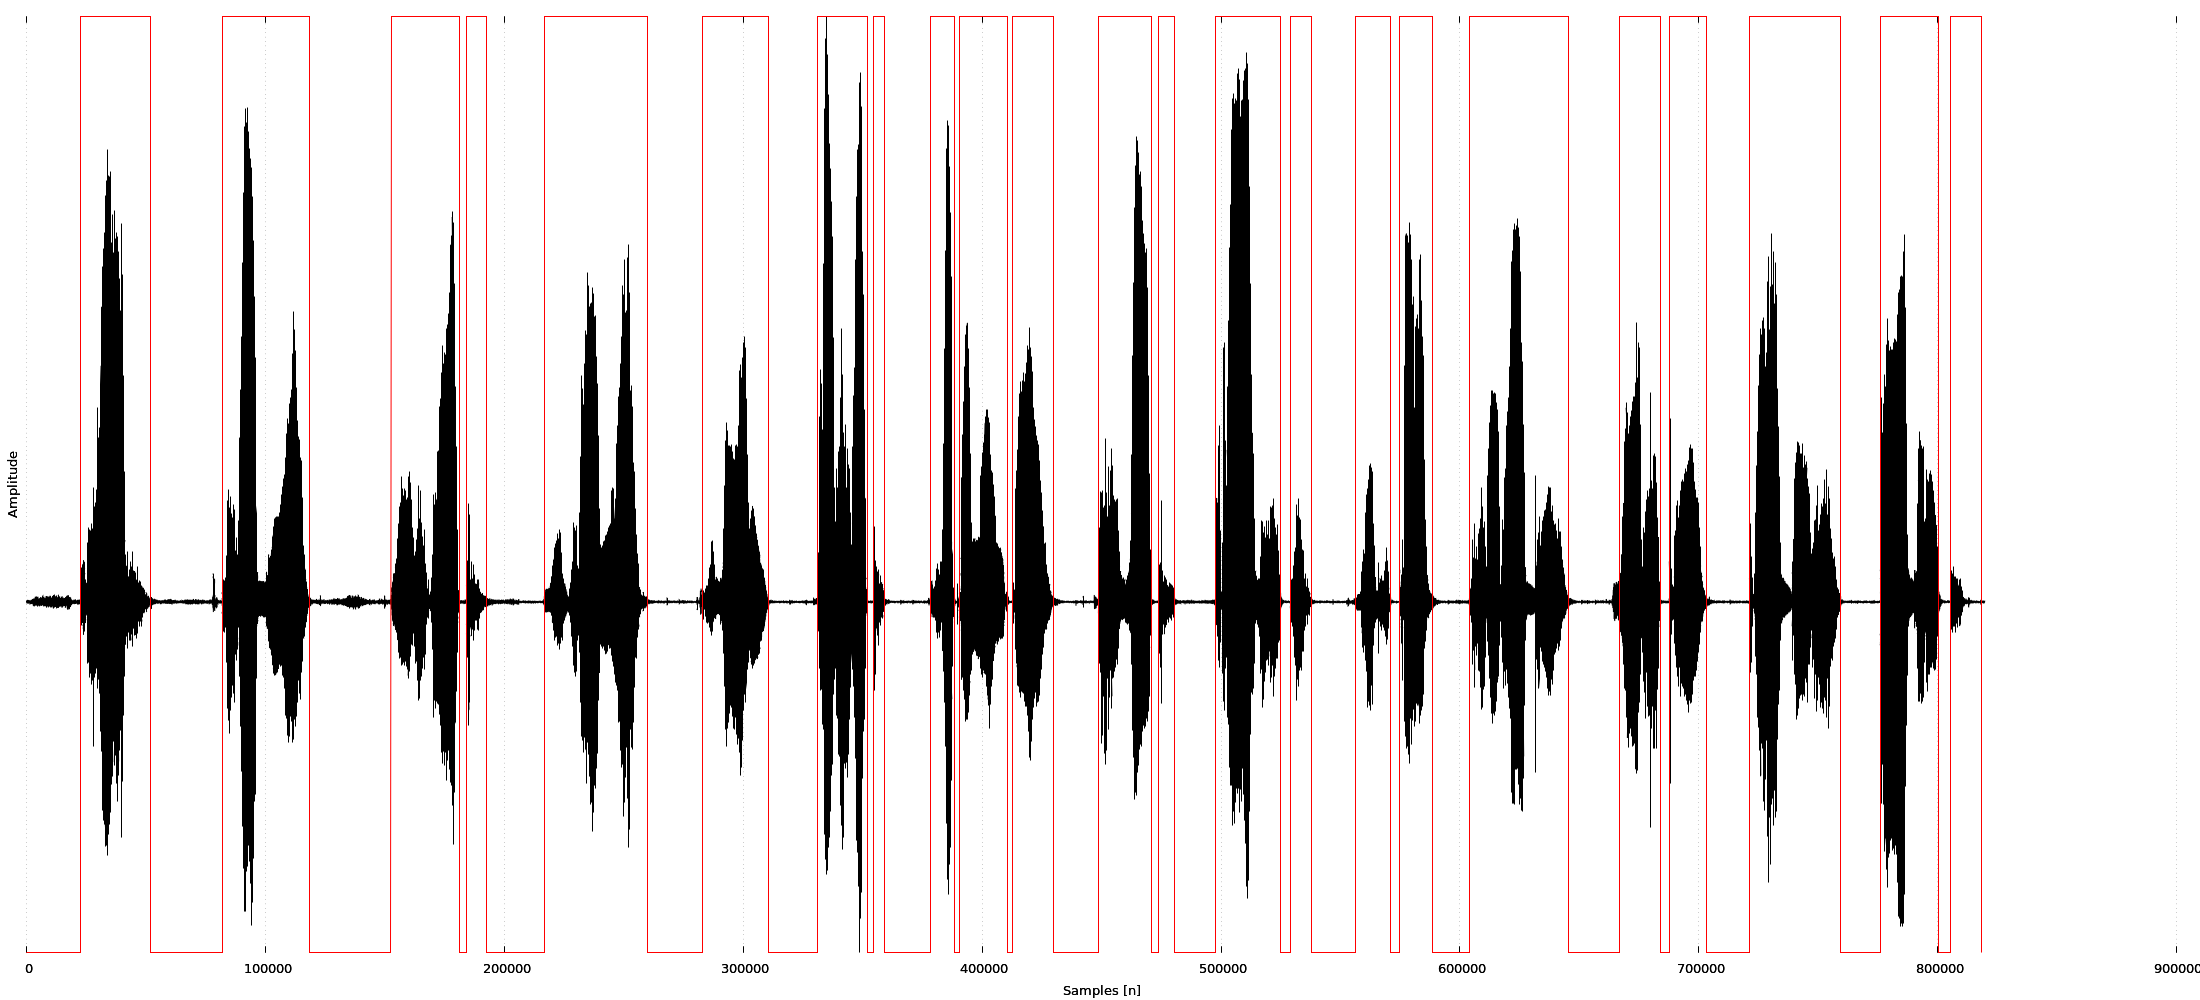
\includegraphics[scale=0.3]{dbi03w1s14wzor.png}}
		\caption{Przebieg czasowy ciągu słów dla głosu damskiego i jego wzorcowa detekcja}\vspace{5mm}
		
		\resizebox{\width}{2cm}{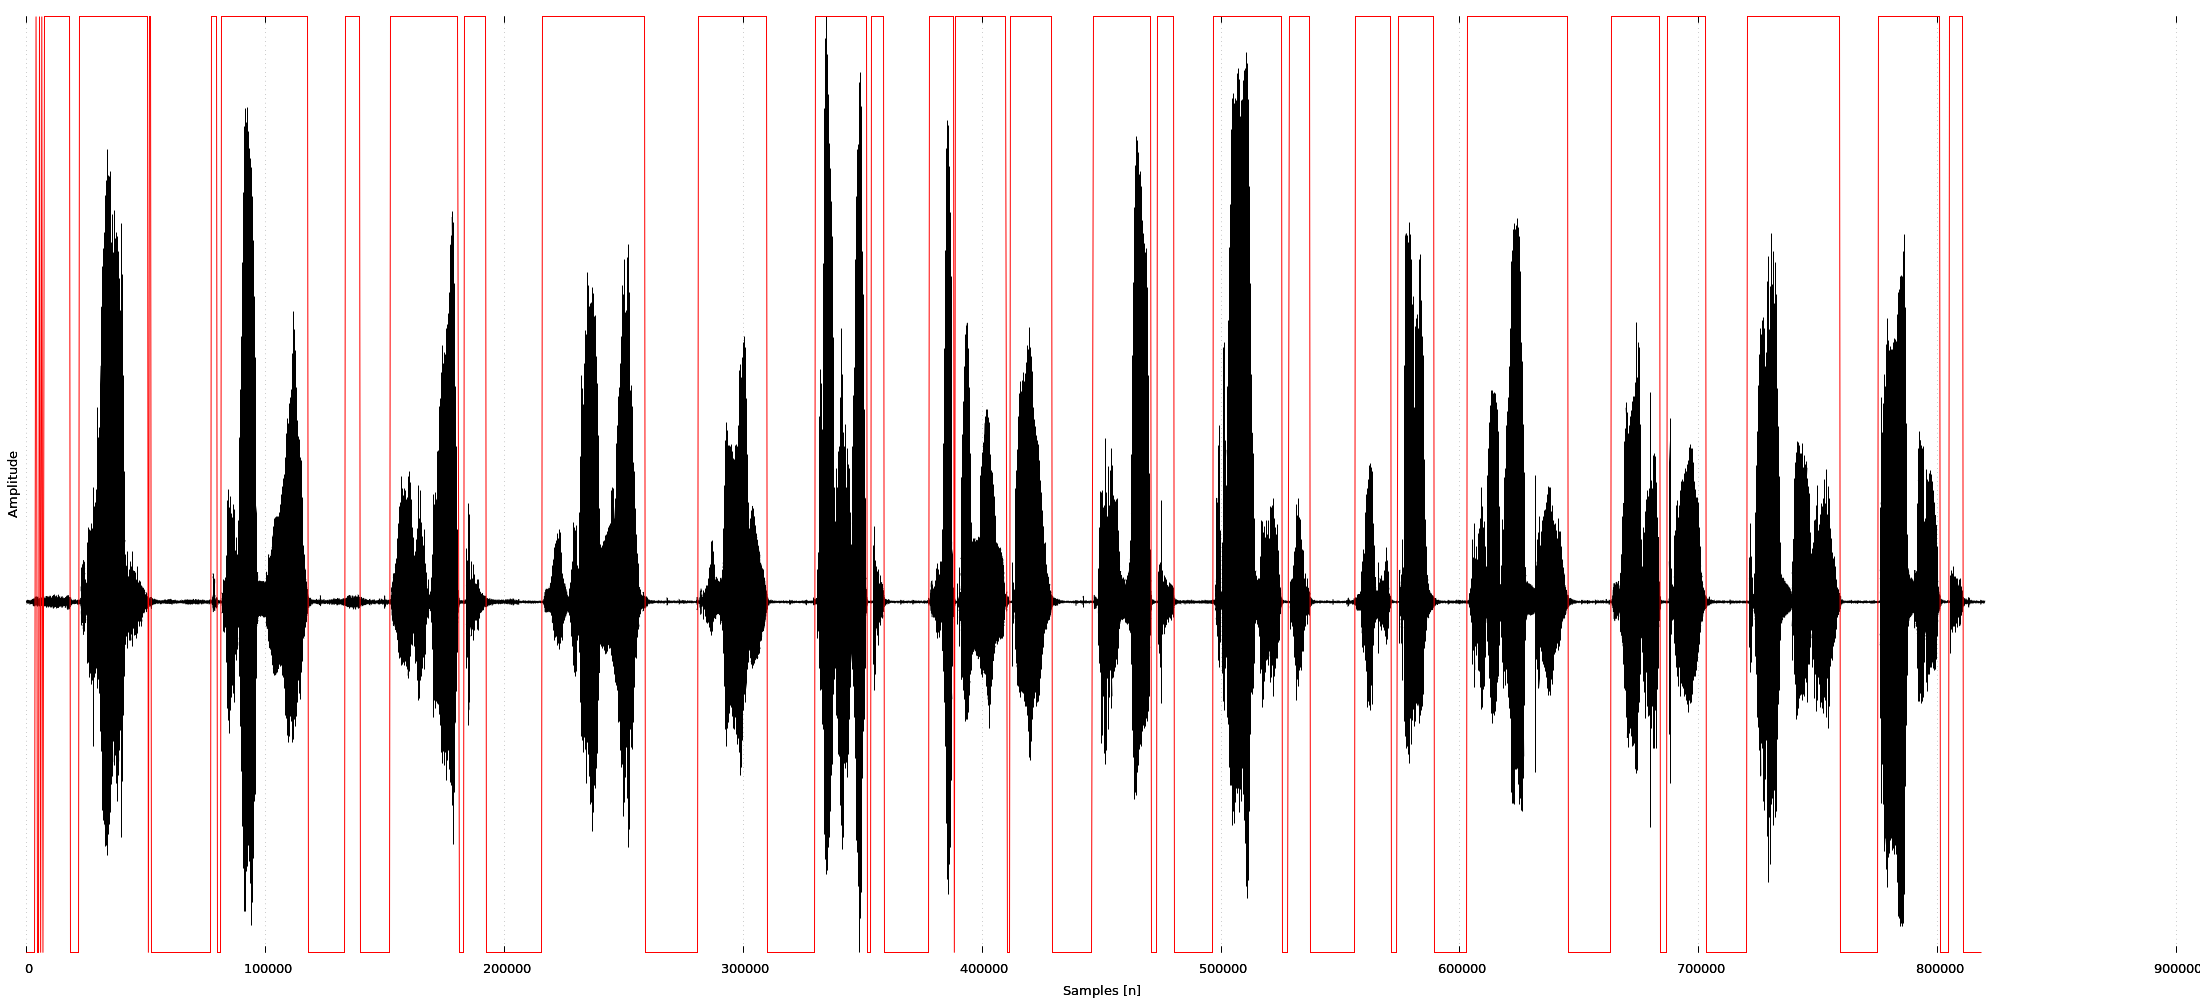
\includegraphics[scale=0.3]{dbi03w1s14Energy.png}}
		\caption{Wynik detekcji algorytmu bazującego na energii sygnału}\vspace{5mm}
		
		\resizebox{\width}{2cm}{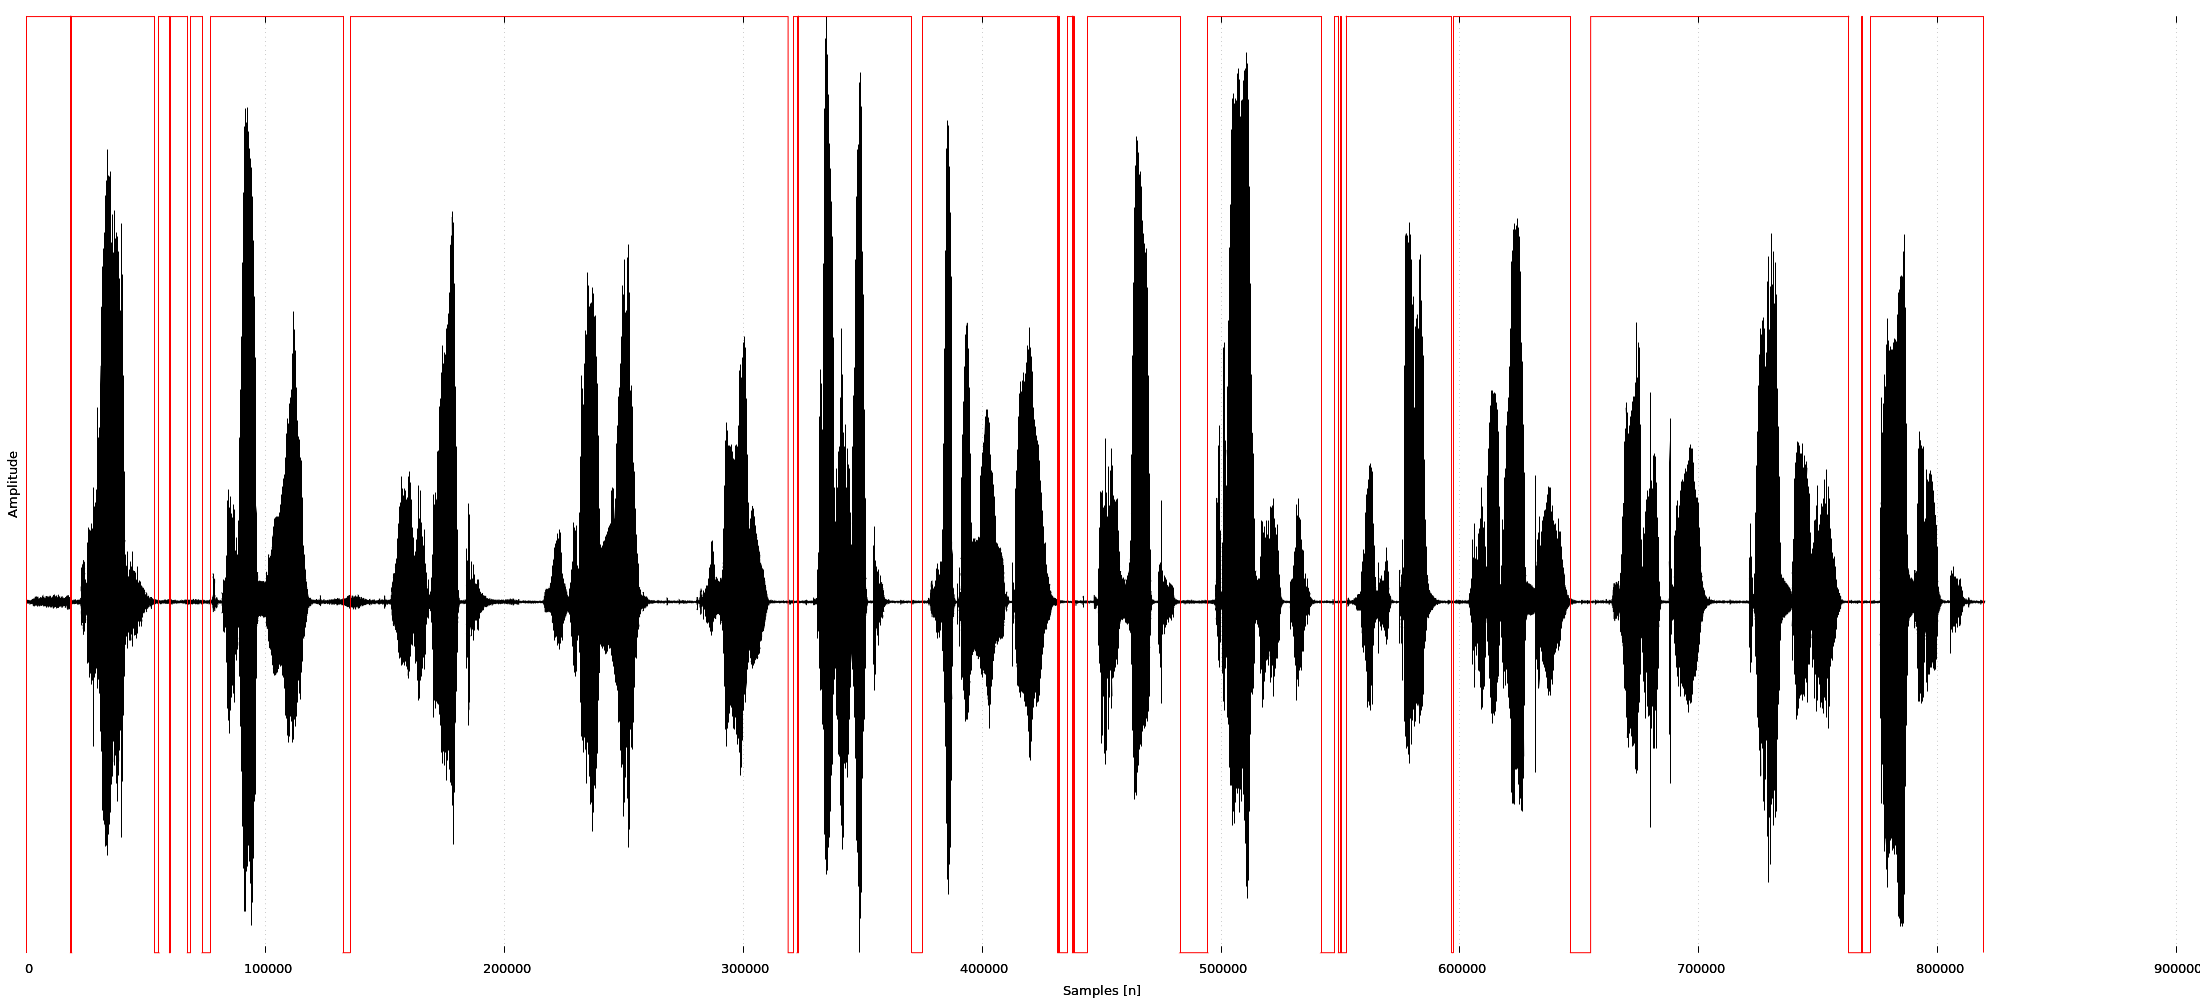
\includegraphics[scale=0.3]{dbi03w1s14SFFArticle.png}}
		\caption{Wynik detekcji algorytmu SFF}\vspace{5mm}
		
		\resizebox{\width}{2cm}{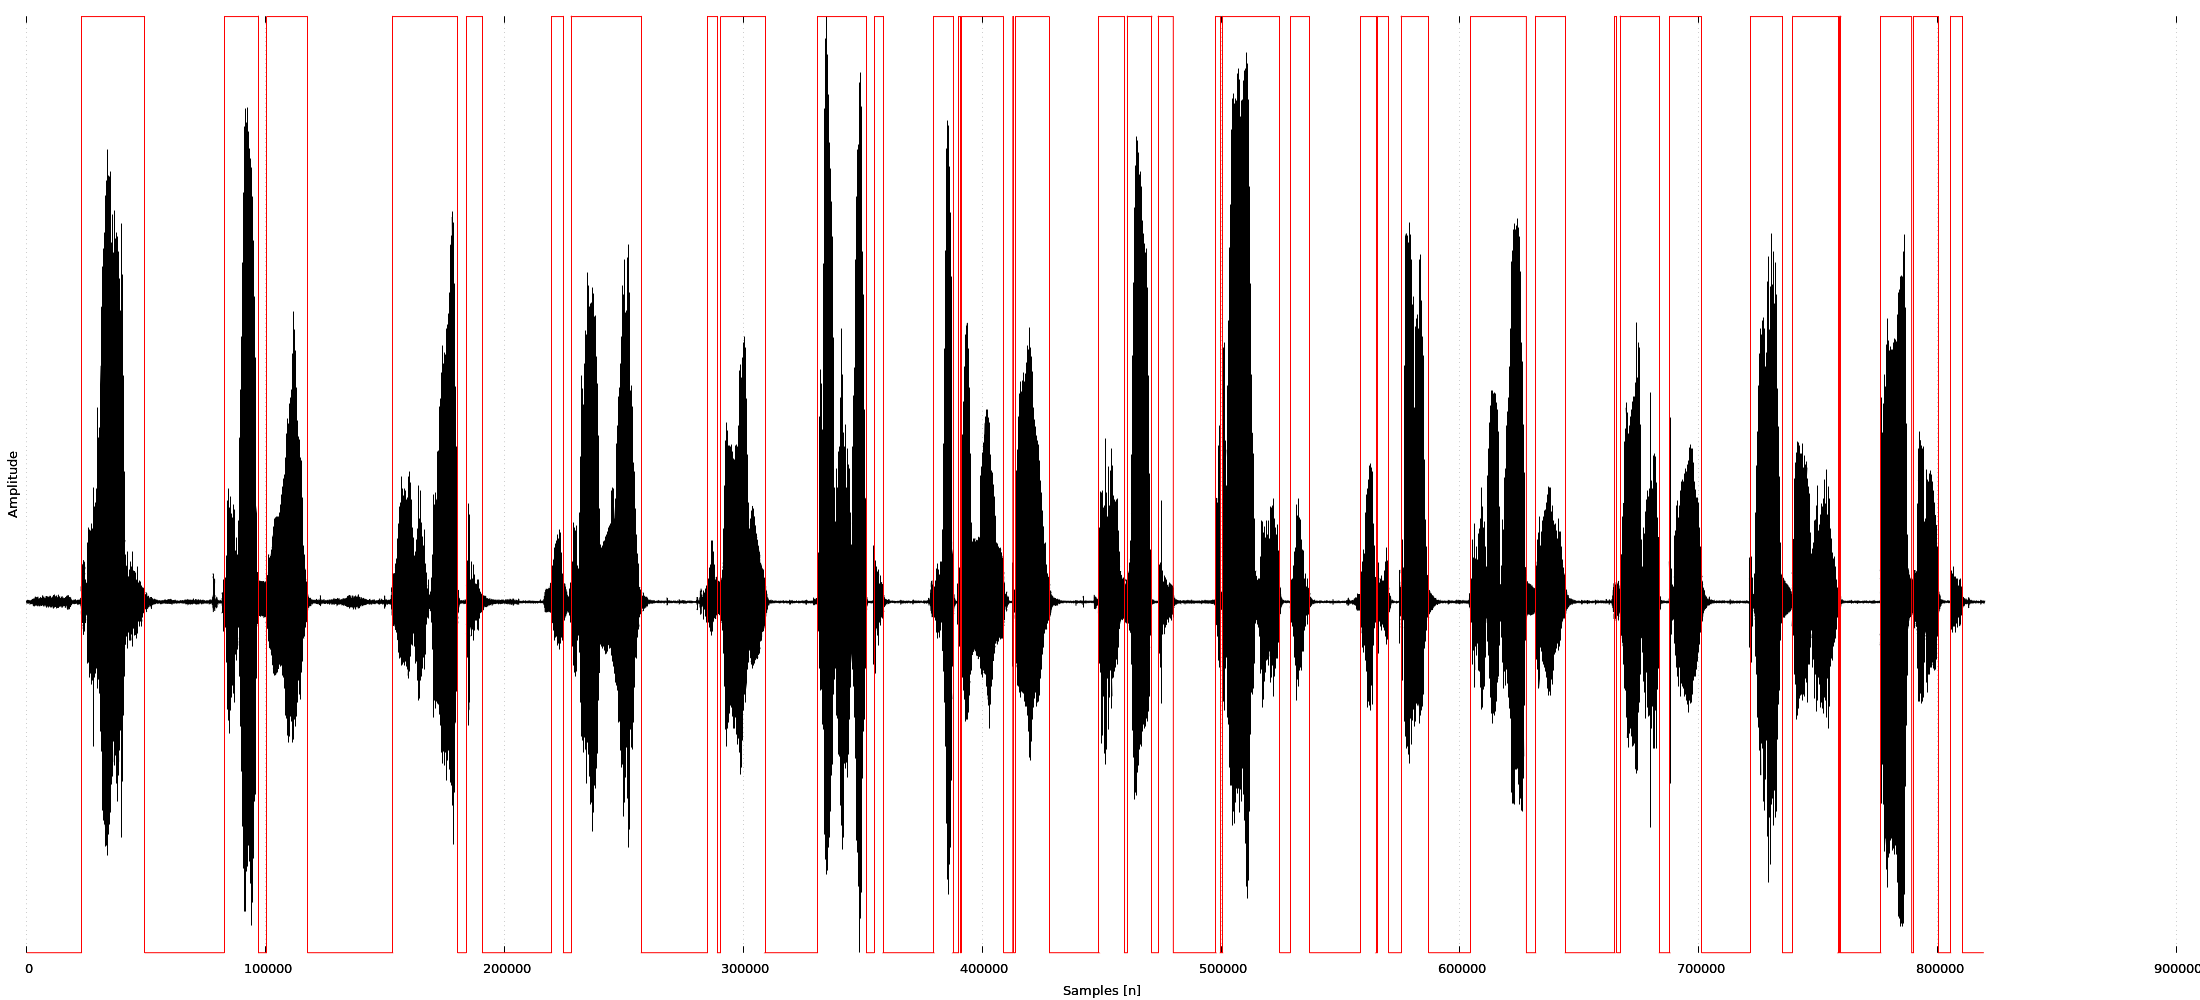
\includegraphics[scale=0.3]{dbi03w1s14SFFChanged.png}}
		\caption{Wynik detekcji algorytmu SFF2}\vspace{5mm}
	\end{center}
\end{sidewaysfigure}


\begin{figure}
	 
	\begin{center}
		$\begin{array}{ | c | c | c | c | c | }
			\hline
			& \textrm{Wzorzec[nr próbki]} & \textrm{En[nr próbki]} & \textrm{SFF[nr próbki]} & \textrm{SFF2[nr próbki]}  \\ \hline
			&22506 & 22080 & 18721 & 23041   \\ \hline
			&51738 & 50880 & 53281 & 49441   \\ \hline
			&82035 & 81600 & 76801 & 82561   \\ \hline
			&118179 & 118080 & 132481 & 117601  \\ \hline
			&152457 & 152160 & 135361 & 153121  \\ \hline
			&181022 & 180960 & & 180481   \\ \hline
			&183927 & 183360 & & 183841   \\ \hline
			&192255 & 192480 & & 190561    \\ \hline
			&216882 & 216000 & & 219841    \\ \hline
			&259958 & 259200 & & 257281    \\ \hline
			&282772 & 281280 & & 285121   \\ \hline
			&310413 & 310080 & 318721 & 309121   \\ \hline
			&330914 & 330240 & 323041 & 331201  \\ \hline
			&351839 & 351840 & 370561 & 351361   \\ \hline
			& 354455 & 353760 & & 354721  \\ \hline
			& 359172 & 359040 & & 358561   \\ \hline
			& 378238 & 377760 & 374881 & 379681  \\ \hline
			& 388346 & 388320 & & 387841  \\ \hline
			& 390280 & 388800 & & 390241  \\ \hline
			& 410592 & 410400 & & 408961  \\ \hline
			& 412623 & 411840 & & 412801  \\ \hline
			& 429792 & 429600 & 431521 &  428161  \\ \hline
			& 448556 & 446400 & 444001 &  448801  \\ \hline
			& 470851 & 470880 & & 470881   \\ \hline
			& 473898 & 473280 & & 473761  \\ \hline
			& 480523 & 480480 & 482881 & 480001  \\ \hline
			& 497692 & 496800 & 494401 & 497761  \\ \hline
			& 525016 & 525600 & & 524641 \\ \hline
			& 528933 & 528480 & & 528961  \\ \hline
			& 537880 & 537600 & 541921 & 537121   \\ \hline
			& 556209 & 556320 & 552481 & 558241   \\ \hline
			& 570960 & 571200 & & 570241  \\ \hline
			& 574780 & 574080 & & 575521  \\ \hline
			& 588322 & 589440 & 596641 & 587041  \\ \hline
			& 603943 & 603360 & 597121 & 604321  \\ \hline
			& 645333 & 645600 & 646081 & 644161  \\ \hline
			& 666836 & 663360 & 654721 & 664801  \\ \hline
			& 683855 & 684000 & & 683521   \\ \hline
			& 687597 & 686880 & & 687841  \\ \hline
			& 703231 & 703200 & & 701281  \\ \hline
			& 721172 & 720480 & & 721441 \\ \hline
			& 759463 & 759360 & 762721 & 759361   \\ \hline
			& 775968 & 775200 & 771841 & 776161  \\ \hline
			& 800470 & 801120 & & 800161 \\ \hline
			& 805494 & 804960 & & 805441 \\ \hline
			& 818400 & 810720 & 819360 & 810241   \\ \hline
			$\bfseries$\textrm{SUMA RÓŻNIC} &$\bfseries 0$ &$\bfseries 33957$ &$\bfseries 136271$ &$\bfseries 45403$ \\ \hline
			$\bfseries$\textrm{Ilość detekcji} &$\bfseries 46$ &$\bfseries 60$ &$\bfseries 44$ &$\bfseries 72$ \\ \hline
			$\bfseries$ \textrm{Wynik} &$\bfseries 0 $&$\bfseries 34657$ &$\bfseries 136371$ &$\bfseries 46703$ \\ \hline
		\end{array}$
		\caption{Wyniki detekcji algorytmów dla ciągu słów, głos damski}
	\end{center}
	
\end{figure}
\begin{sidewaysfigure}
	\begin{center}
		\resizebox{\width}{2cm}{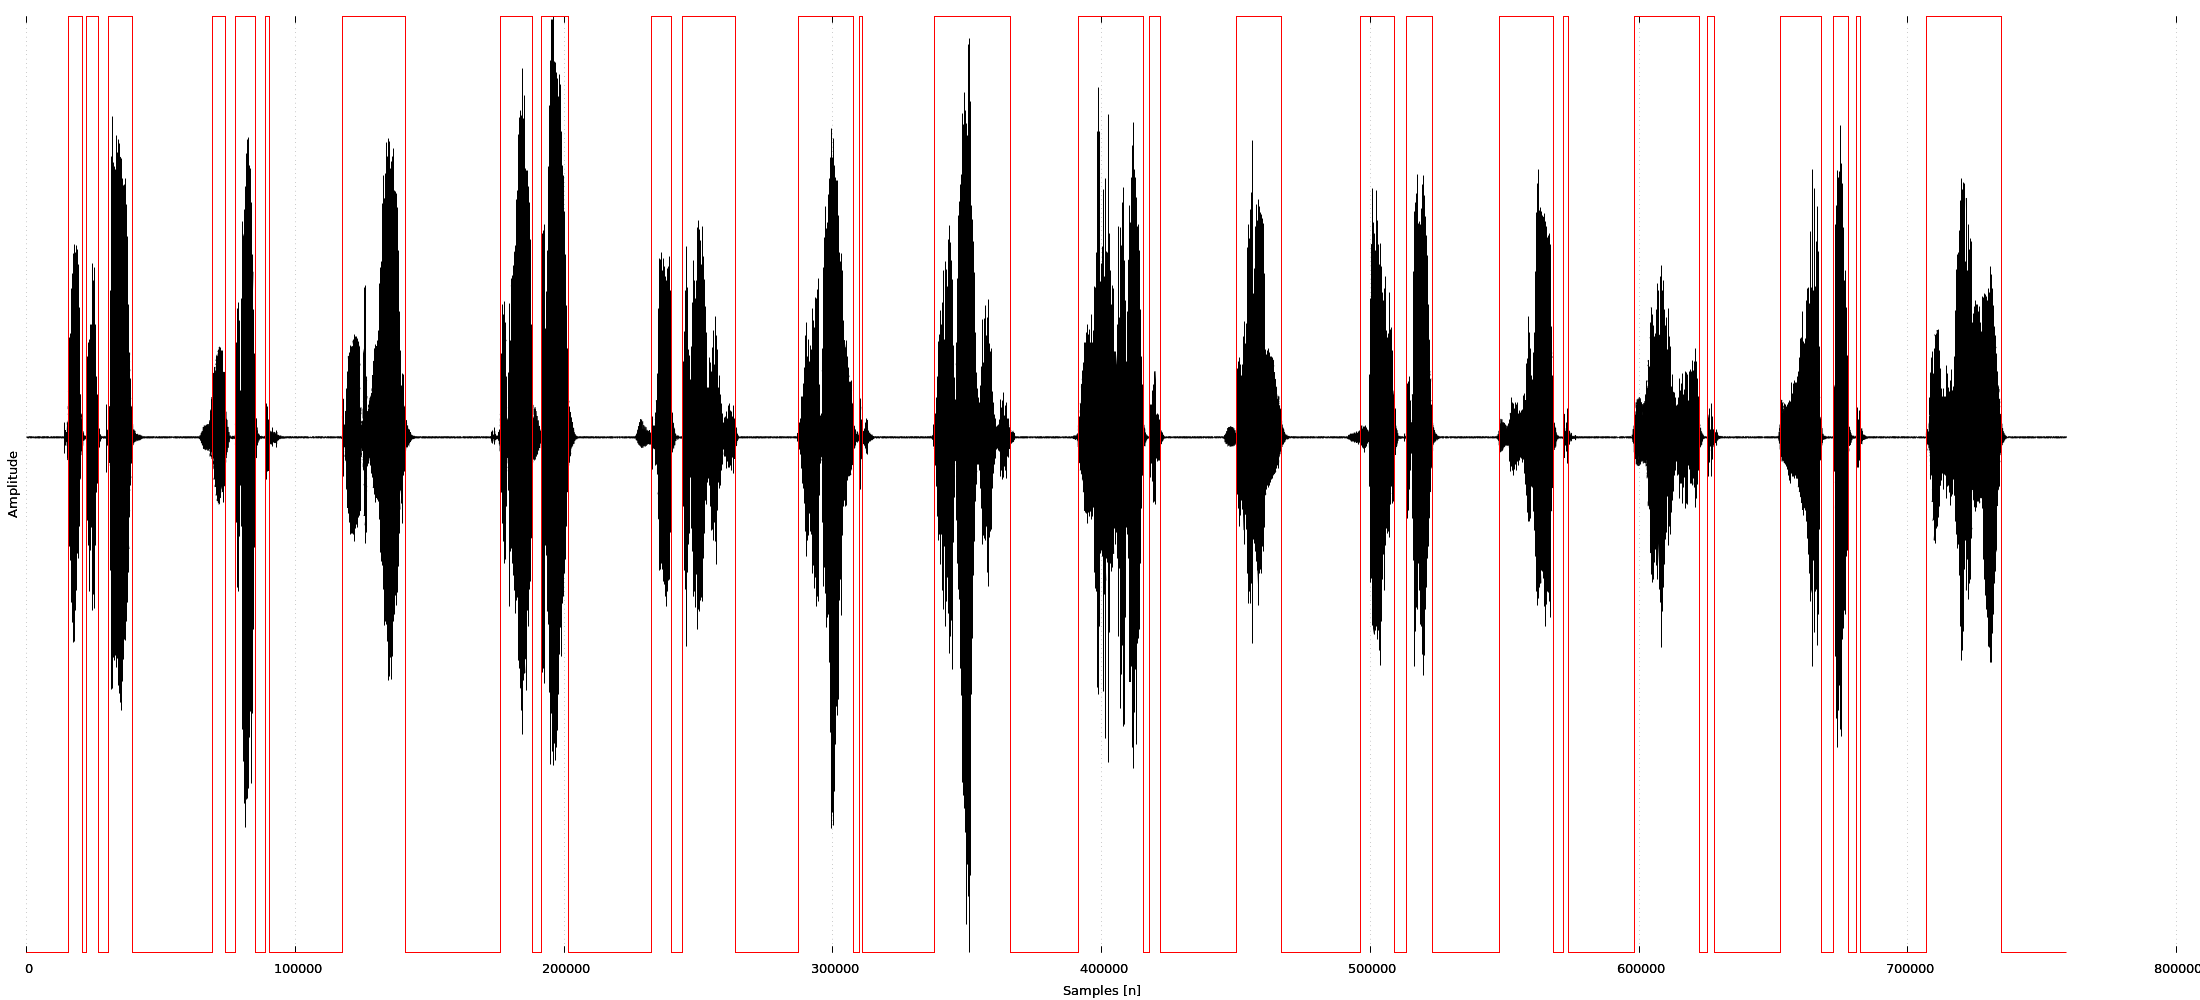
\includegraphics[scale=0.3]{mwr35w1s14wzor.png}}
		\caption{Przebieg czasowy ciągu słów dla głosu damskiego i jego wzorcowa detekcja}\vspace{5mm}
		
		\resizebox{\width}{2cm}{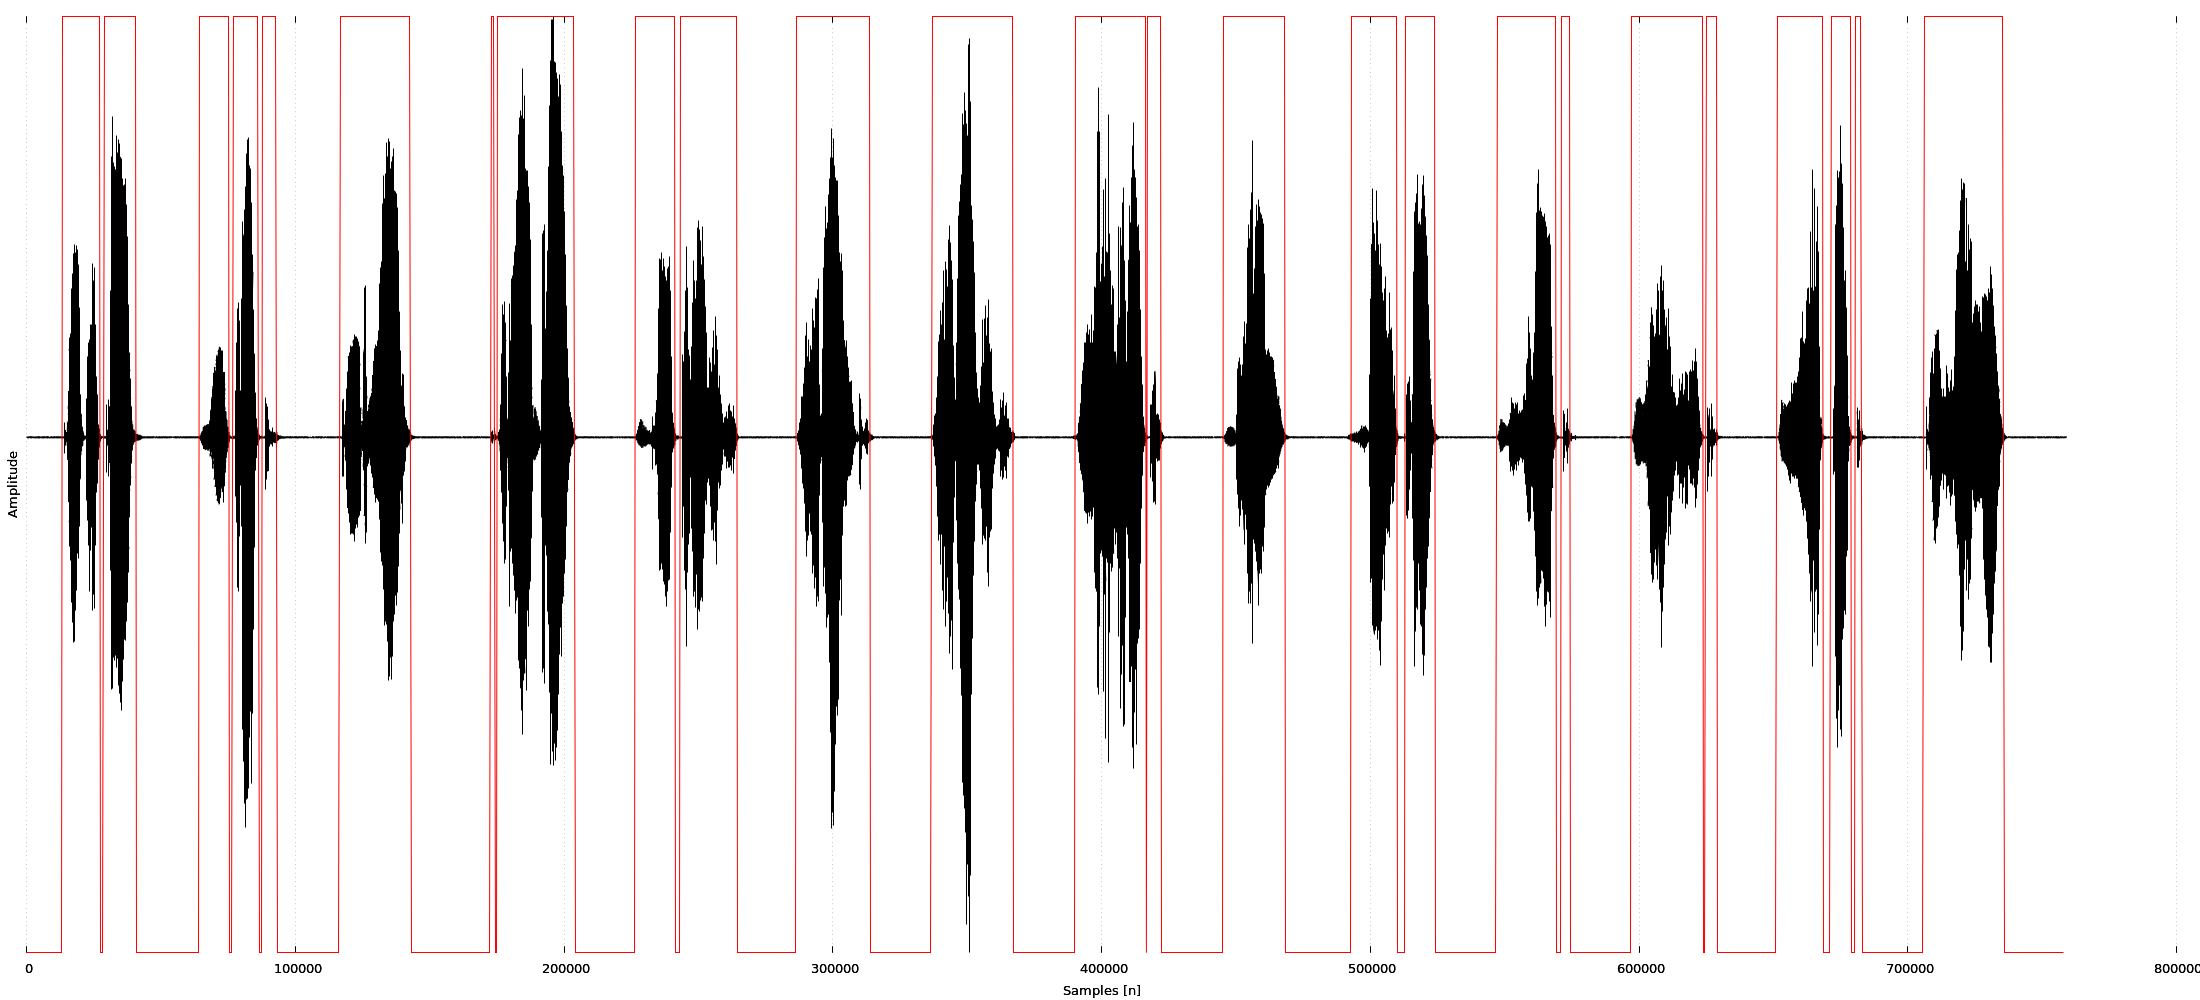
\includegraphics[scale=0.3]{mwr35w1s14Energy.png}}
		\caption{Wynik detekcji algorytmu bazującego na energii sygnału}\vspace{5mm}
		
		\resizebox{\width}{2cm}{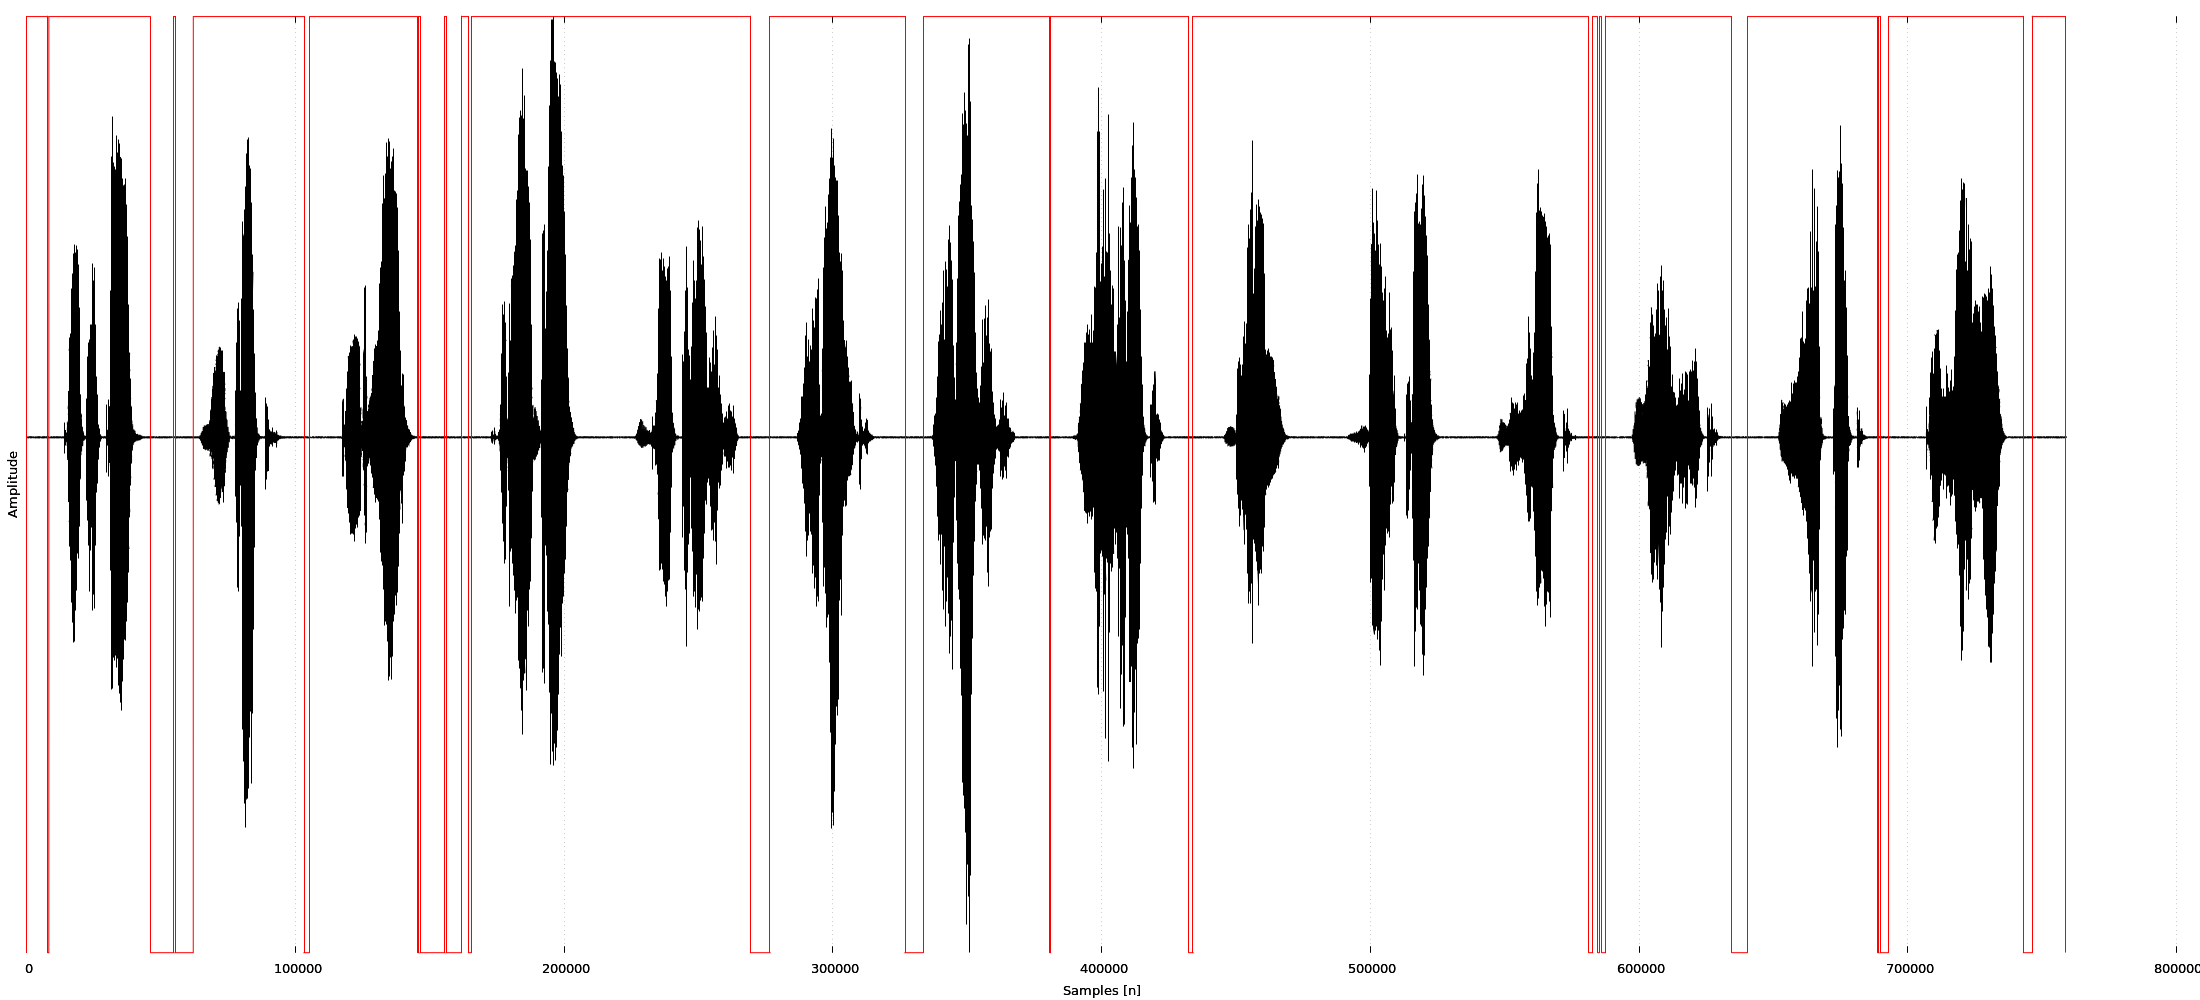
\includegraphics[scale=0.3]{mwr35w1s14SFFArticle.png}}
		\caption{Wynik detekcji algorytmu SFF}\vspace{5mm}
		
		\resizebox{\width}{2cm}{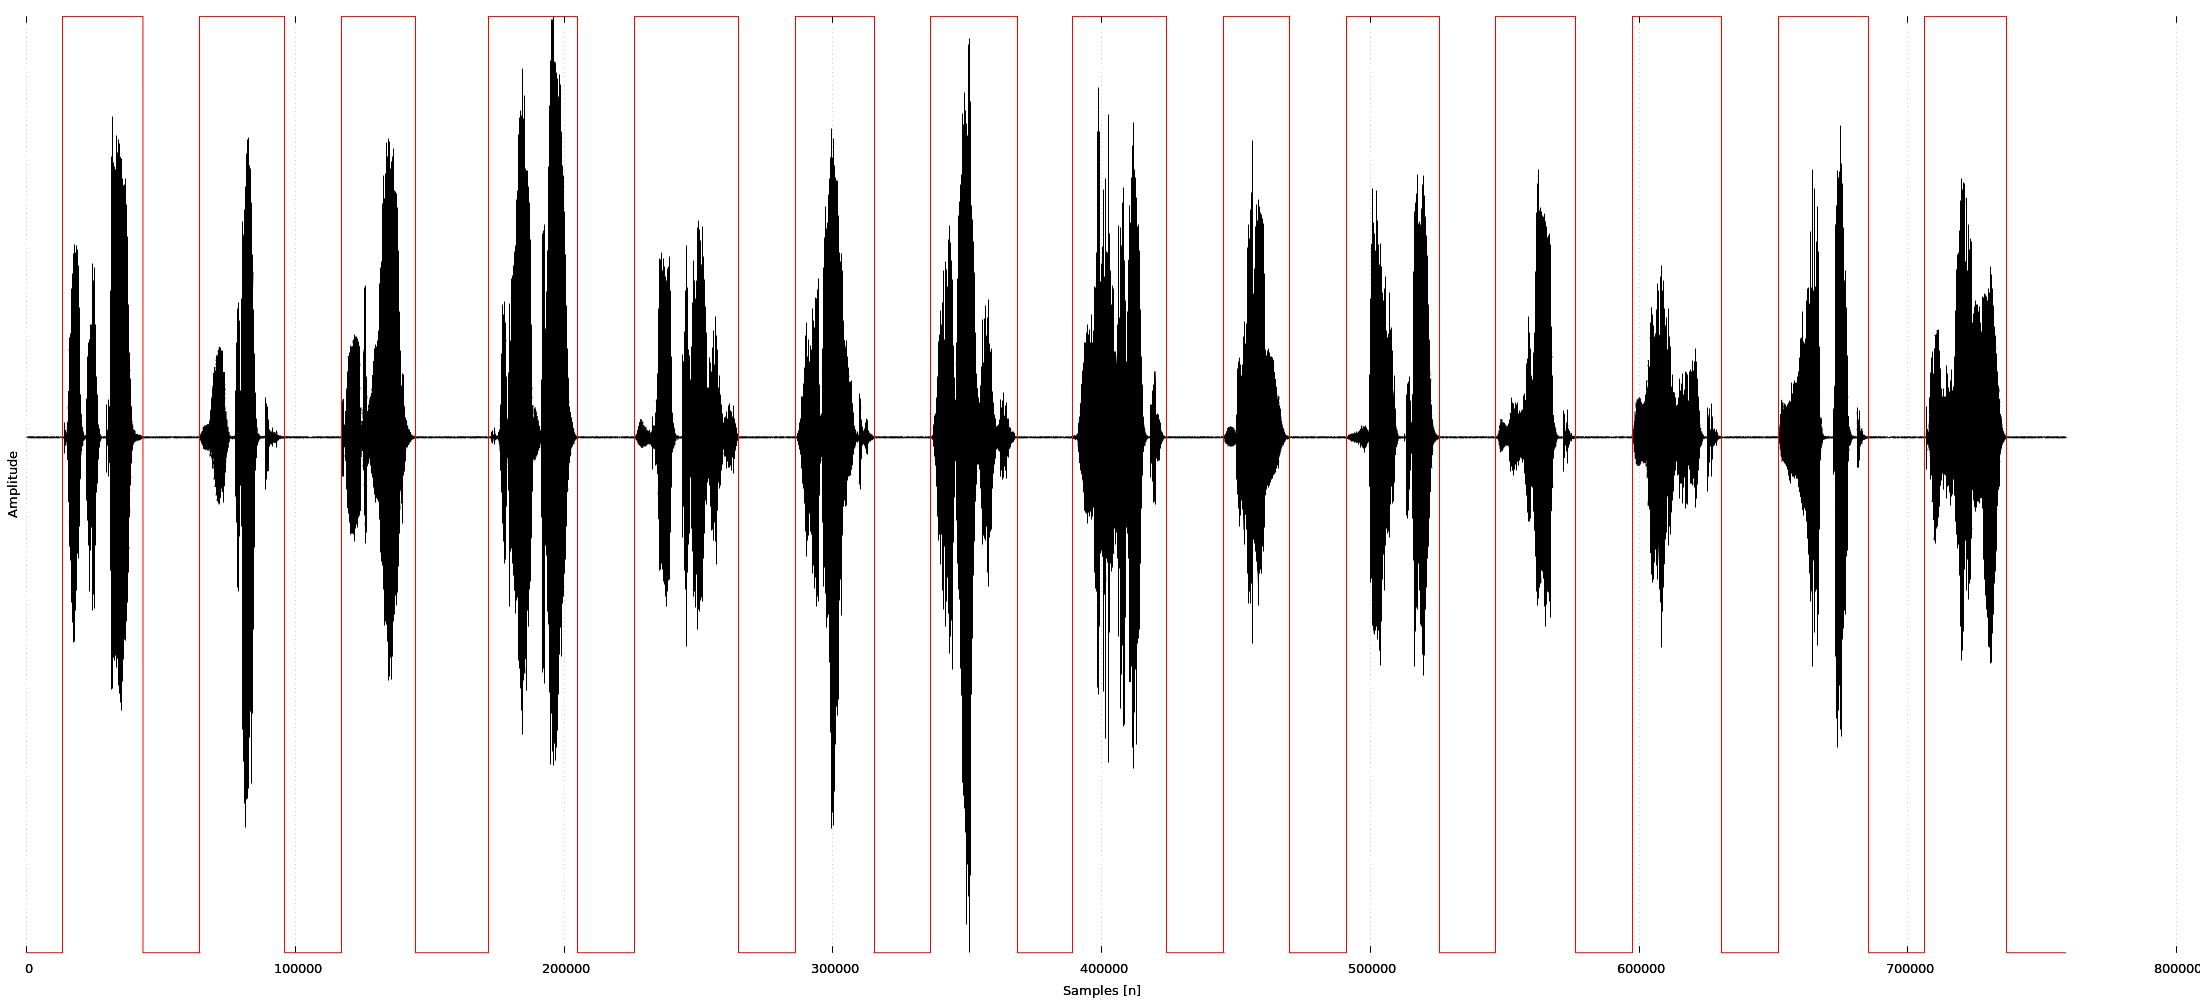
\includegraphics[scale=0.3]{mwr35w1s14SFFChanged.png}}
		\caption{Wynik detekcji algorytmu SFF2}\vspace{5mm}
	\end{center}
\end{sidewaysfigure}


\begin{figure}
	\footnotesize
	\begin{center}
		$\begin{array}{ | c | c | c | c | c | }
		\hline
		& \textrm{Wzorzec} & \textrm{En[nr probki]} & \textrm{SFF[nr probki]} & \textrm{SFF2[nr probki]} \\ \hline
		& 15306 & 13440 & 8161 & 13441  \\ \hline
		& 20545 & & &   \\ \hline
		& 22161 & & &    \\ \hline
		& 26800 & 27360 & &   \\ \hline
		& 30362 & 28800 & &   \\ \hline
		& 39144 & 40800 & 46081 & 43201   \\ \hline
		& 68926 & 64320 & 61921 & 64321   \\ \hline
		& 74062 & 75360 & &   \\ \hline
		& 77542 & 76800 & &   \\ \hline
		& 85080 & 86400 & &  \  \\ \hline
		& 88725 & 87840 & &   \\ \hline
		& 90341 & 93120 & 103201 & 96001  \\ \hline
		& 117389 & 116640 & 105121 & 117121  \\ \hline
		& 140751 & 143040 & 145441 & 144481  \\ \hline
		& 176084 & 175200 & 165601 & 171841  \\ \hline
		& 188096 & & &   \\ \hline
		& 191534 & & & \\ \hline
		& 201600 & 204000 & & 204961   \\ \hline
		& 232500 & 226560 & & 226081   \\ \hline
		& 239956 & 241440 & &   \\ \hline
		& 244140 & 243360 & &   \\ \hline
		& 263732 & 264480 & 269281 & 264961   \\ \hline
		& 287260 & 286560 & 276481 & 286081   \\ \hline
		& 307634 & & &   \\ \hline
		& 309728 & & &   \\ \hline
		& 311125 & 313920 & 326881 & 315361   \\ \hline
		& 337591 & 336960 & 333601 & 336481   \\ \hline
		& 366025 & 367200 & 380641 & 368641   \\ \hline
		& 391540 & 390240 & 381121 & 389281   \\ \hline
		& 415468 & 416640 & &   \\ \hline
		& 417943 & 417120 & &   \\ \hline
		& 421814 & 422400 & 432481 & 424321  \\ \hline
		& 450122 & 445440 & 433921 & 445441  \\ \hline
		& 467068 & 468480 & & 469921  \\ \hline
		& 496200 & 492960 & & 491041  \\ \hline
		& 509084 & 510240 & &  \\ \hline
		& 513591 & 513120 & &  \\ \hline
		& 522984 & 524160 & & 525601 \\ \hline
		& 548054 & 547200 & & 546721 \\ \hline
		& 568174 & 569280 & &   \\ \hline
		& 571918 & 571200 & &  \\ \hline
		& 573696 & 574560 & 581281 & 576481   \\ \hline
		& 598131 & 597120 & 587521 & 597601   \\ \hline
		& 622503 & 624000 & & \\ \hline
		& 625486 & 624960 & &   \\ \hline
		& 627898 & 629280 & 634561 & 630721  \\ \hline
		& 652714 & 651360 & 640321 & 651841  \\ \hline
		& 668010 & 668640 & &   \\ \hline
		& 672390 & 671520 & &   \\ \hline
		& 678102 & 679200 & &  \\ \hline
		& 681085 & 680640 & &   \\ \hline
		& 682291 & 683040 & 688801 & 685441  \\ \hline
		& 706853 & 706080 & 692641 & 706081  \\ \hline
		& 734970 & 735840 & 743041 & 736801  \\ \hline
		$\bfseries$\textrm{SUMA RÓŻNIC} & $\bfseries0$ & $\bfseries 68617$ & $\bfseries 215409$ & $\bfseries 78751$ \\ \hline
		$\bfseries$\textrm{Ilość detekcji} &$\bfseries 54$ &$\bfseries 50$ &$\bfseries 40$ &$\bfseries 28$ \\ \hline
		$\bfseries$\textrm{Wynik} & $\bfseries0$ & $\bfseries 68814$ & $\bfseries 216109$ &$\bfseries 80051$ \\ \hline
		\end{array}
		$
		\caption{Wyniki detekcji algorytmów dla ciągu słów, głos męski}
	\end{center}
	
\end{figure}

\begin{figure}
\section{Powtórzenie badań przy większym poziomie zaszumienia}
W wyniku osiągnięcia zadowalających efektów działania algorytmów na sygnałach z minimalnym poziomem zaszumienia, postanowiono sprawdzić, jakie wyniki dzadzą zastosowane na sygnałach o dużo wyższym poziomie zaszumienia. Zastosowano do tego szum Gaussowski o średniej $\mu = 0.0$  oraz o odchyleniu standardowym $\sigma=1000$
\end{figure}

\begin{sidewaysfigure}
	\begin{center}
		\resizebox{\width}{2cm}{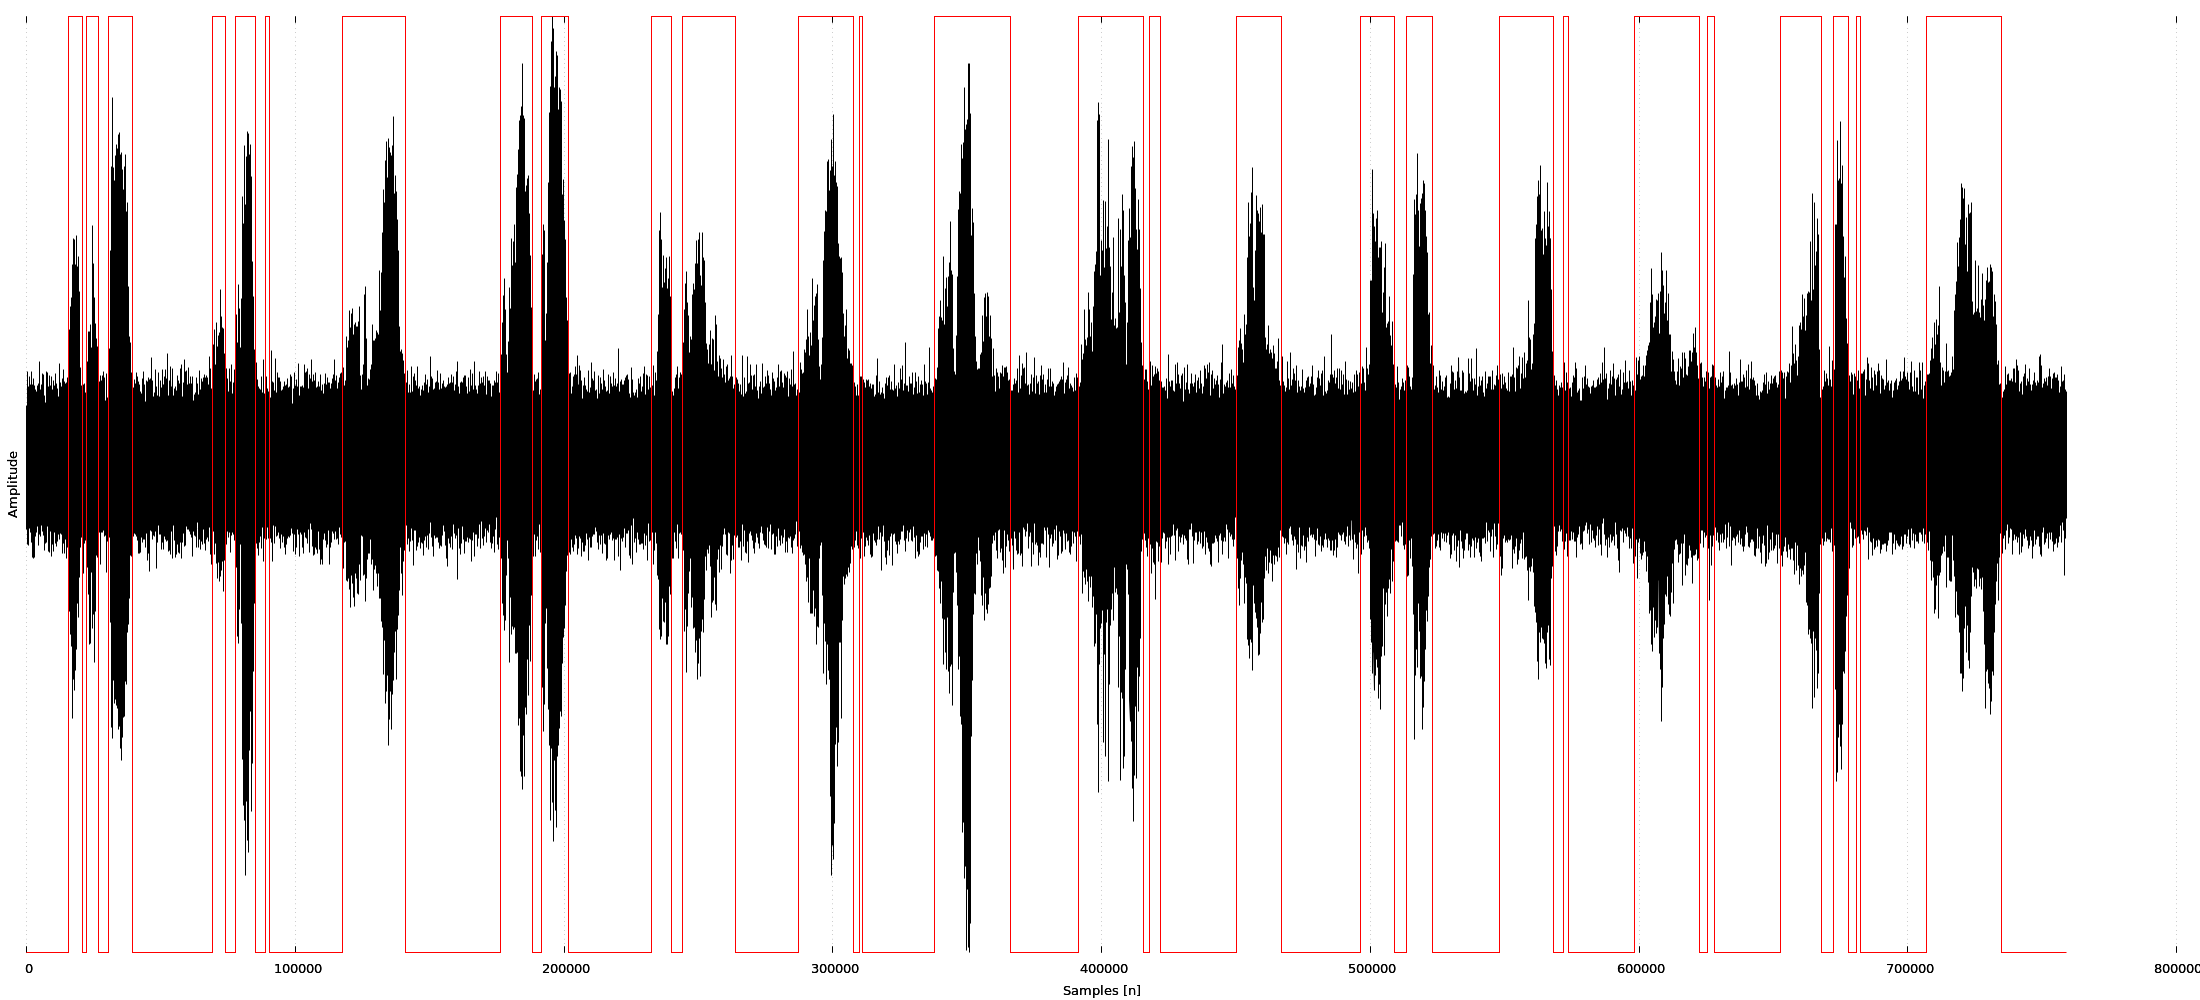
\includegraphics[scale=0.3]{noisemwr35w1s14wzor.png}}
		\caption{Przebieg czasowy ciągu słów dla głosu męskiego i jego wzorcowa detekcja}\vspace{5mm}
		
		\resizebox{\width}{2cm}{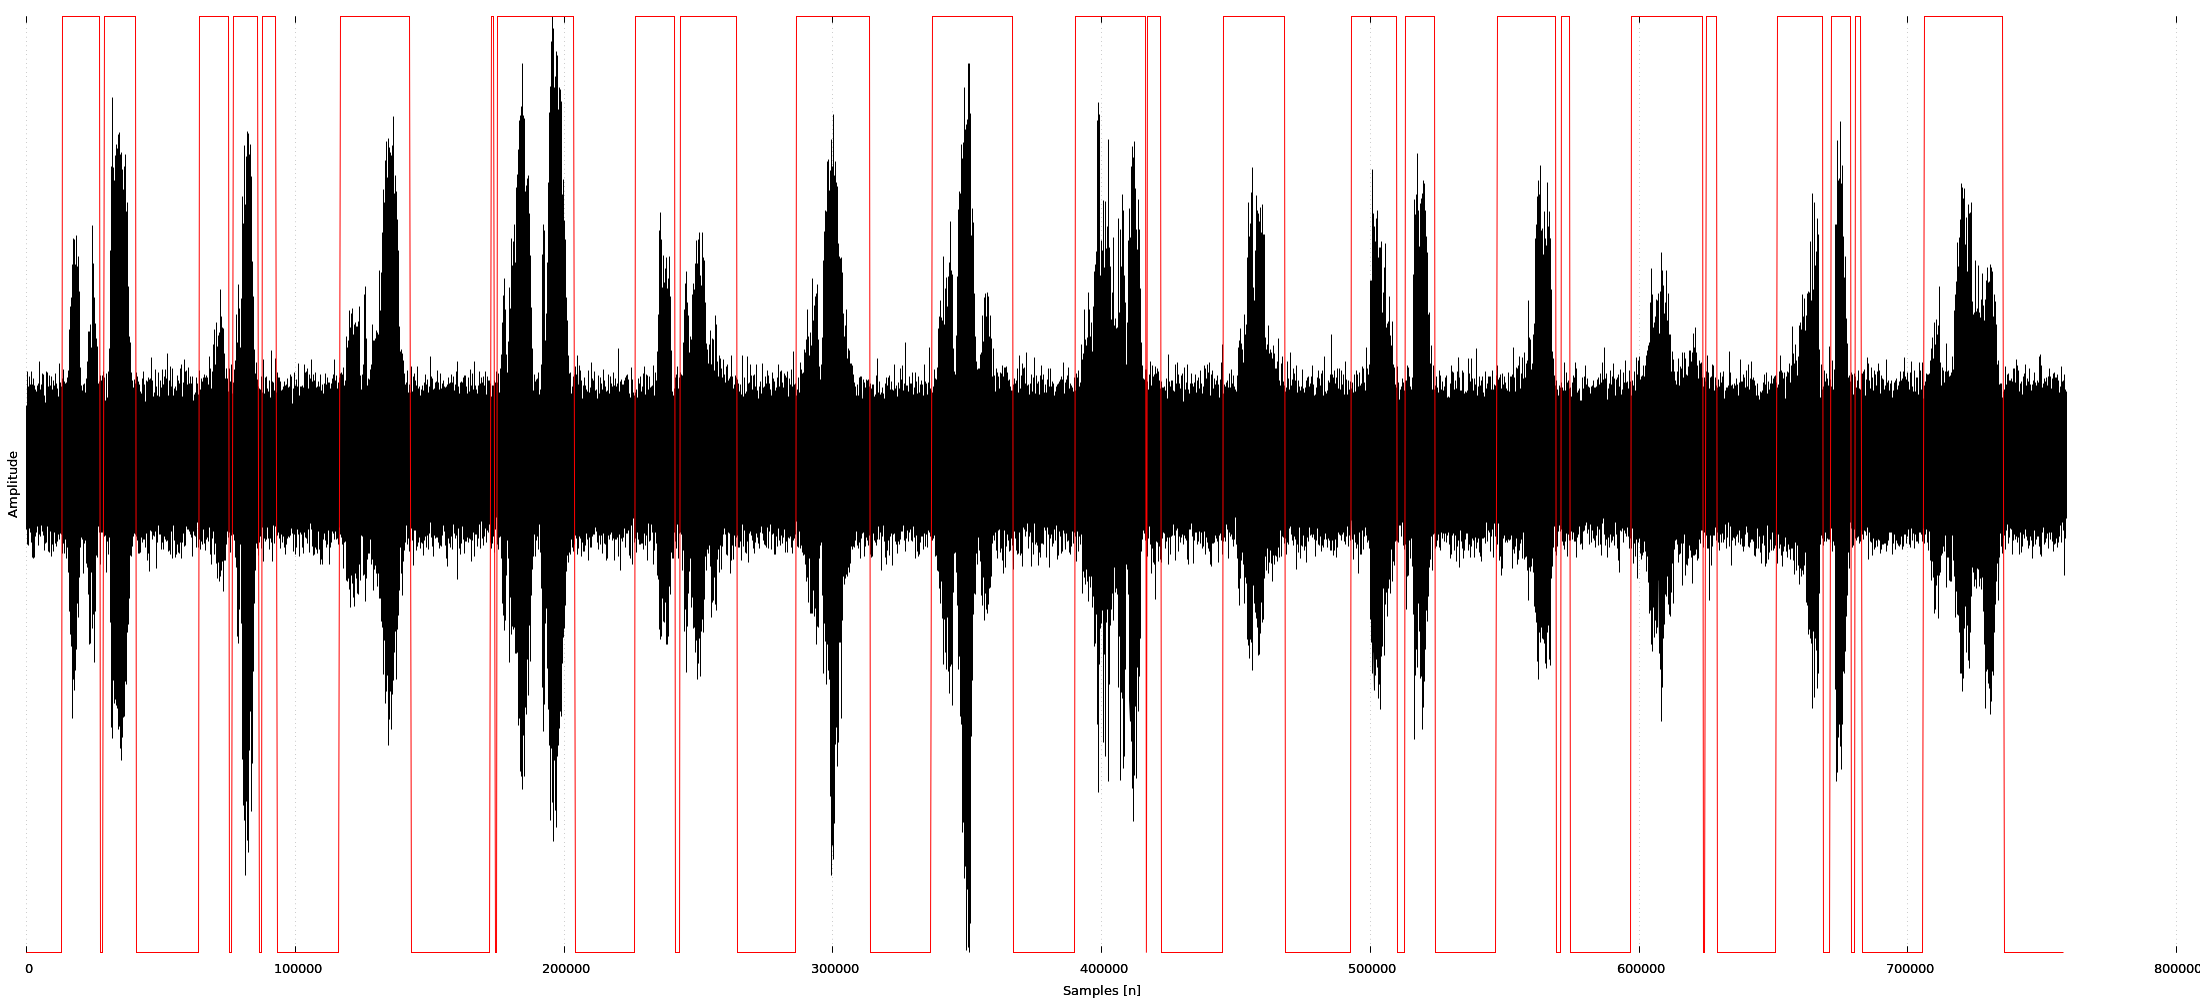
\includegraphics[scale=0.3]{noisemwr35w1s14Energy.png}}
		\caption{Wynik detekcji algorytmu bazującego na energii sygnału}\vspace{5mm}
		
		\resizebox{\width}{2cm}{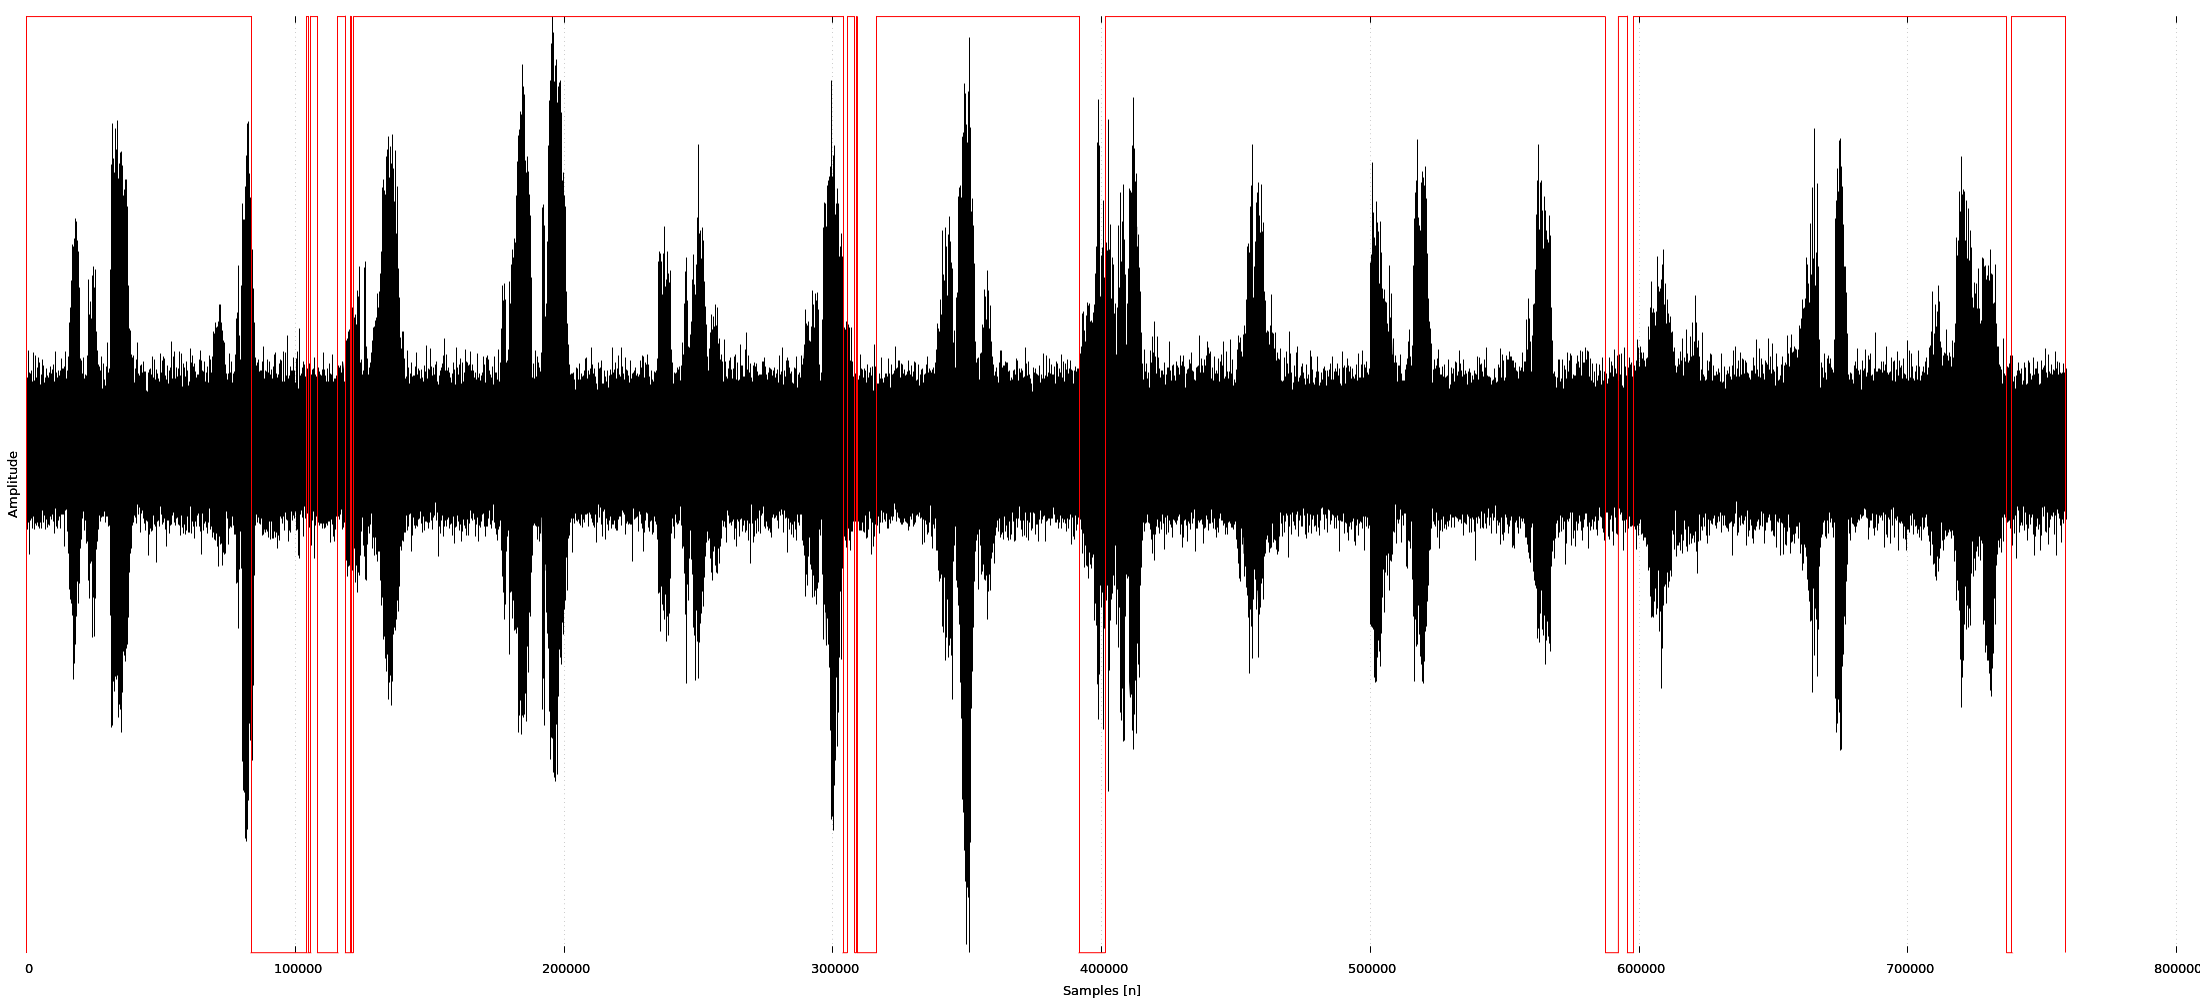
\includegraphics[scale=0.3]{noisemwr35w1s14SFFArticle.png}}
		\caption{Wynik detekcji algorytmu SFF}\vspace{5mm}
		
		\resizebox{\width}{2cm}{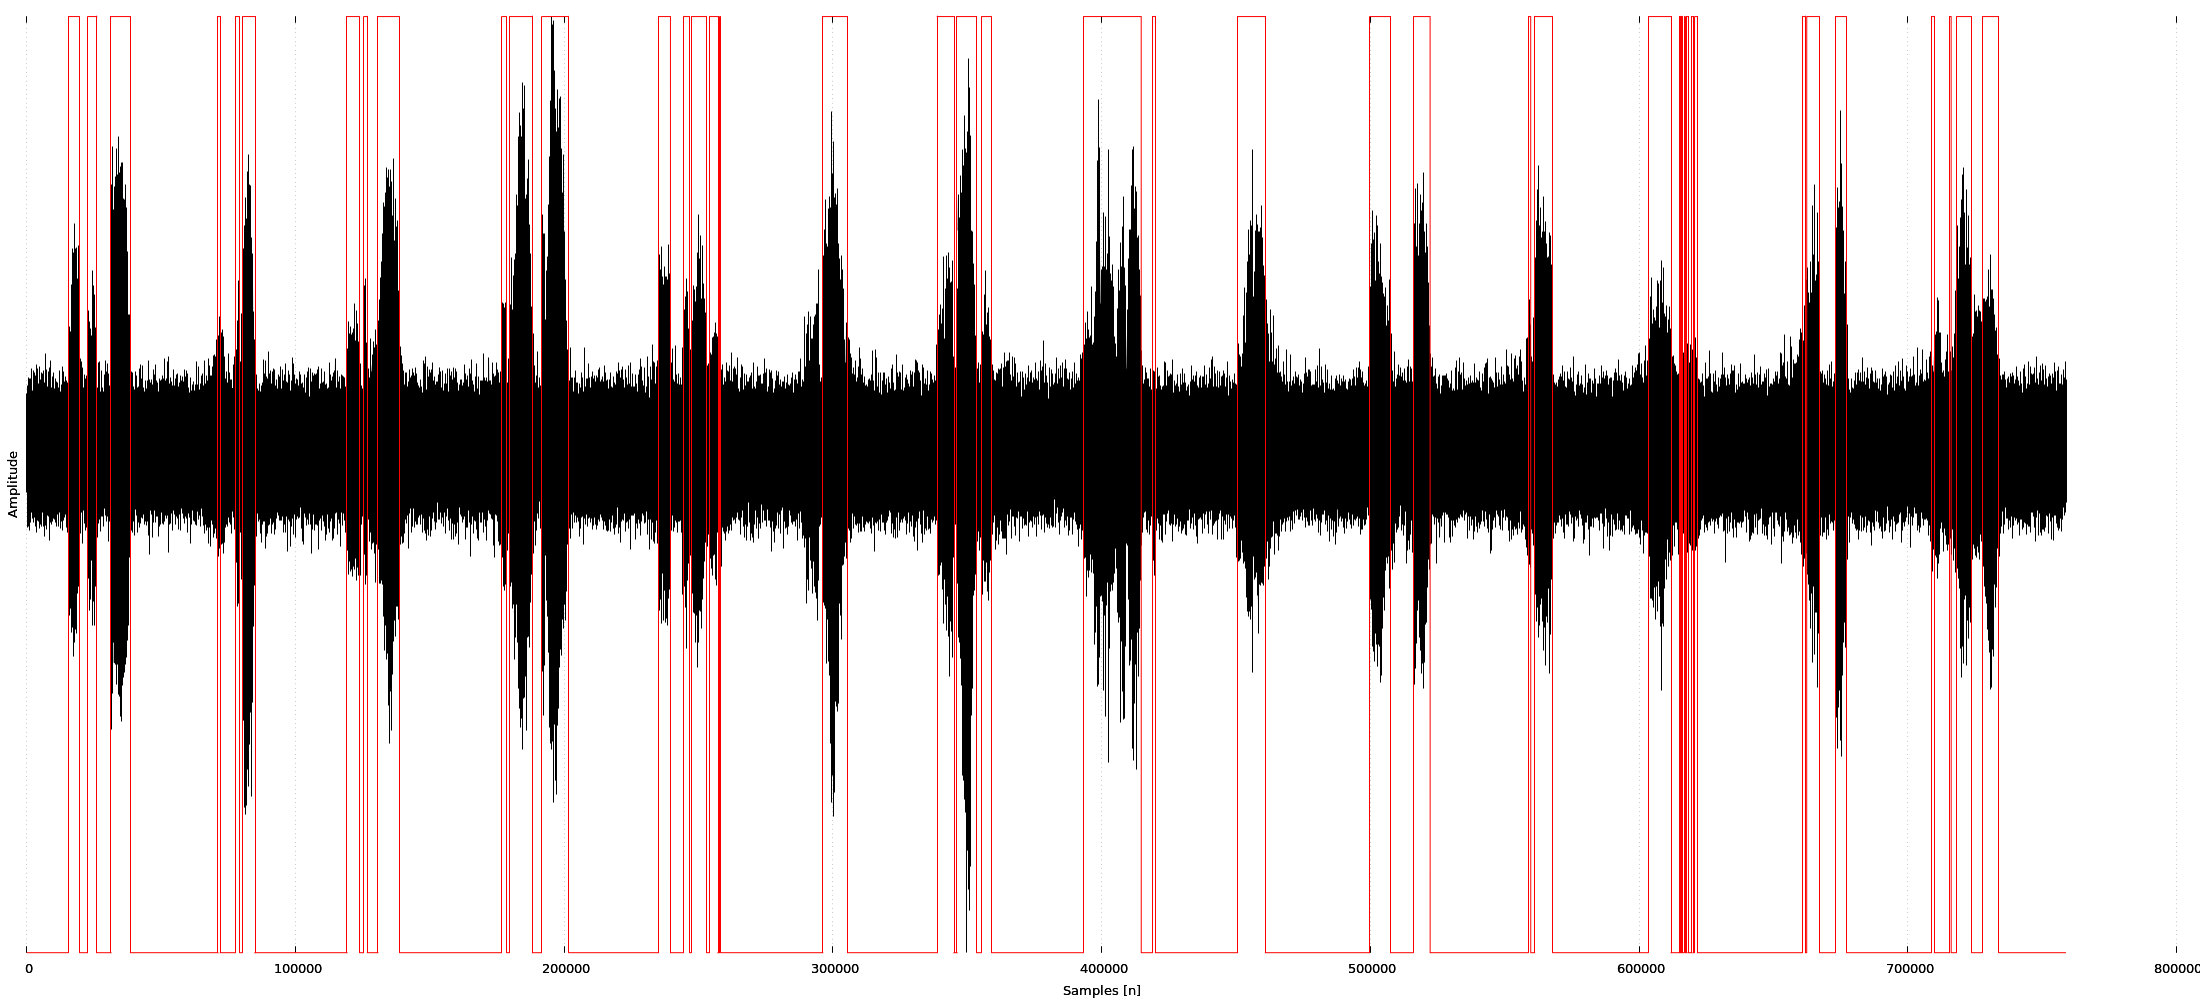
\includegraphics[scale=0.3]{noisemwr35w1s14SFFChanged.png}}
		\caption{Wynik detekcji algorytmu SFF2}\vspace{5mm}
	\end{center}
\end{sidewaysfigure}


\begin{figure}
	\footnotesize
	\begin{center}
		$
		\begin{array}{ | c | c | c | c | c | }
		\hline
		& wzorzec & En[nr probki] & SFF[nr probki] & SFF2[nr probki]  \\ \hline
		& 15306 & 13440 & 2 & 15361   \\ \hline
		& 20545 & & & 19681  \      \\ \hline
		& 22161 & & & 22561 \    \\ \hline
		& 26800 & 27360 & & 25921 \    \\ \hline
		& 30362 & 28800 & & 31201  \   \\ \hline
		& 39144 & 40800 & & 38401  \    \\ \hline
		& 68926 & 64320 & & 71041  \    \\ \hline
		& 74062 & 75360 & & 72001  \    \\ \hline
		& 77542 & 76800 & & 77761  \    \\ \hline
		& 85080 & 86400 & 83521 & 79201   \\ \hline
		& 88725 & 87840 & & 80161  \    \\ \hline
		& 90341 & 93120 & & 84961  \    \\ \hline
		& 117389 & 116640 & 121441 & 119041  \\ \hline
		& 140751 & 143040 & & 138721  \    \\ \hline
		& 176084 & 175200 & & 179521  \   \\ \hline
		& 188096 & & & 188161  \    \\ \hline
		& 191534 & & & 191521 \    \\ \hline
		& 201600 & 204000 & & 201601  \    \\ \hline
		& 232500 & 226560 & & 235201  \    \\ \hline
		& 239956 & 241440 & & 239521  \   \\ \hline
		& 244140 & 243360 & & 244321  \    \\ \hline
		& 263732 & 264480 & & 258241  \   \\ \hline
		& 287260 & 286560 & 303841 & 296161  \\ \hline
		& 307634 & & 305281 & 305281  \    \\ \hline
		& 309728 & \  & \  & \    \\ \hline
		& 311125 & 313920 & \  & \    \\ \hline
		& 337591 & 336960 & 316321 & 338881 \\ \hline
		& 366025 & 367200 & 391681 & 359041 \\ \hline
		& 391540 & 390240 & 401281 & 393121 \\ \hline
		& 415468 & 416640 & & 414721  \   \\ \hline
		& 417943 & 417120 & & 419041  \   \\ \hline
		& 421814 & 422400 & & 420001  \   \\ \hline
		& 450122 & 445440 & & 450721  \   \\ \hline
		& 467068 & 468480 & & 460801  \   \\ \hline
		& 496200 & 492960 & & 499681  \   \\ \hline
		& 509084 & 510240 & & 507361  \   \\ \hline
		& 513591 & 513120 & & 516001  \   \\ \hline
		& 522984 & 524160 & & 522241  \   \\ \hline
		& 548054 & 547200 & & 558721  \   \\ \hline
		& 568174 & 569280 & & 567841  \   \\ \hline
		& 571918 & 571200 & \  & \   \\ \hline
		& 573696 & 574560 & 587521 & \   \\ \hline
		& 598131 & 597120 & 598081 & 603361  \\ \hline
		& 622503 & 624000 & & 612001  \   \\ \hline
		& 625486 & 624960 & & 614881  \   \\ \hline
		& 627898 & 629280 & & 615361  \   \\ \hline
		& 652714 & 651360 & & 660961  \   \\ \hline
		& 668010 & 668640 & & 667201  \   \\ \hline
		& 672390 & 671520 & & 672961  \   \\ \hline
		& 678102 & 679200 & & 677281  \   \\ \hline
		& 681085 & 680640 & \  & \   \\ \hline
		& 682291 & 683040 & \  & \   \\ \hline
		& 706853 & 706080 & & 708961  \  \\ \hline
		& 734970 & 735840 & 736801 & 733921  \\ \hline
		$\bfseries \textrm{SUMA RÓŻNIC}$& $\bfseries 0$ & $\bfseries 68614$ & $\bfseries 112222$ & $\bfseries 147473$ \\ \hline
		$\bfseries \textrm{Ilość detekcji}$ & $\bfseries 54$ & $\bfseries50$ &$\bfseries 26$ &$\bfseries 84$ \\ \hline
		$\bfseries {Wynik}$ &$\bfseries 0$ &$\bfseries 68814$ &$\bfseries 113622$ &$\bfseries 148973$ \\ \hline
		\end{array}
		$
		\caption{Wyniki detekcji algorytmów dla ciągu słów, głos męski, większy szum}
	\end{center}
	
\end{figure}
\chapter{Podsumowanie}

W celu lepszego zobrazowania otrzymanych rezultatów zostały wygenerowane wykresy przedstawiające wartość wskaźnika błędu dla każdego z algorytmów. Ostatni wykres przedstawia sumę wszystkich wyników dla każdego z badanych algorytmów.
Z przeprowadzonych badań wynika, że najlepsze wyniki detekcji daje algorytm oparty o energię sygnału. Na drugim miejscu znalazł się zmieniony algorytm SFF, a na końcu oryginalny SFF. Poniższe wykresy prezentują różnicę w dokładności detekcji algorytmów:

\begin{figure}
	\begin{center}
		{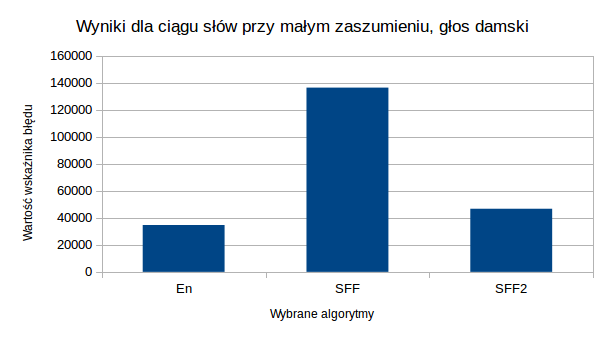
\includegraphics[scale=1]{dbi03w1s14results.png}}
		\caption{Wyniki dla ciągu słów, głos damski, małe zaszumienie}\vspace{5mm}
	\end{center}
\end{figure}

\begin{figure}
	\begin{center}
		{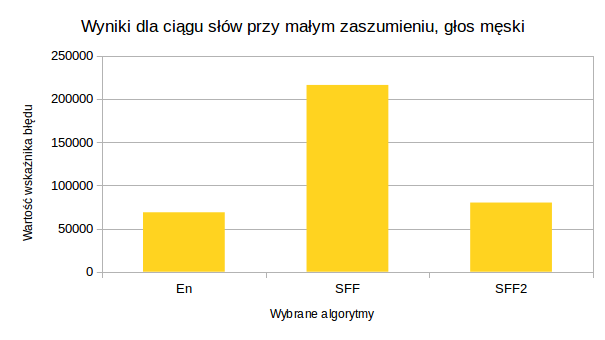
\includegraphics[scale=1]{mwr35w1s14results.png}}
		\caption{Wyniki dla ciągu słów, głos męski, małe zaszumienie}\vspace{5mm}
	\end{center}
\end{figure}


\begin{figure}
	\begin{center}
		{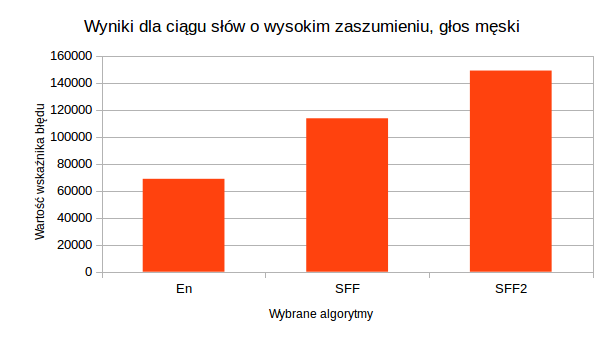
\includegraphics[scale=1]{noisedmwr35w1s14results.png}}
		\caption{Wyniki dla ciągu słów, głos męski, duże zaszumienie}\vspace{5mm}
	\end{center}
\end{figure}


\begin{figure}
	\begin{center}
		{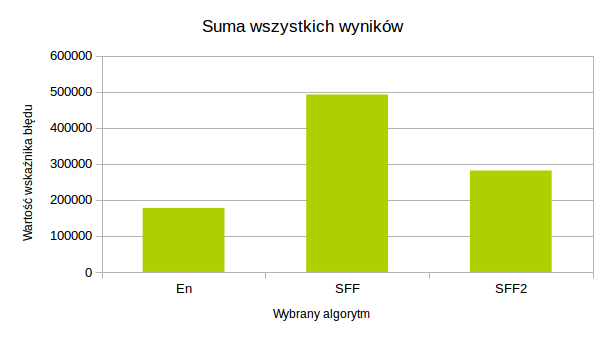
\includegraphics[scale=1]{sumOfResults.png}}
		\caption{Suma wyników wszystkich kolejnych badań}\vspace{5mm}
	\end{center}
\end{figure}

\chapter{Dodatek A - Implementacja}
Do zaimplementowania algorytmów skorzystano z biblioteki Aquila, która wspiera wykonywanie operacji na sygnałach. Poza tym, użyto standardowych bibliotek C++, takich jak cmath, STL.

\section{Algorytm oparty o energię sygnału}
Implementacja algorytmu bazującego na energii sygnału była dośc prosta i jego główna idea, czyli dynamicznie zmieniający się próg, jest zawarta w następujących liniach kodu:
\lstset{language=C++,basicstyle=\scriptsize}
\begin{lstlisting}
//DELTA = 1.00
void EnergyBased::calculateThresholdEminEmax(Aquila::WaveFile wav,
size_t currentFrameNumber) {
	
	double singleFrameEnergy=frameEn.countSingleFrameEnergy(wav,currentFrameNumber);
	
	//if it's first frame
	if(currentFrameNumber==0) {
		initialValue = singleFrameEnergy;
		if(initialValue==0){
			initialValue = 1;
			Emax = initialValue;
			Emin = initialValue;
		}else {
			Emax = initialValue;
			Emin = initialValue;
		}
	}	
	if(currentFrameNumber>0){
		delta=delta*1.0001;
		Emin=Emin*delta;
	}
	//if frame energy is higher than Emax
	if(singleFrameEnergy>Emax){
		Emax=singleFrameEnergy;
	}
	//if frame energy is lower than Emin
	else if(singleFrameEnergy<Emin) {
		if(singleFrameEnergy==0){
			Emin=initialValue;
			//resetDelta
			delta=DELTA;
		}
		else{
			Emin=singleFrameEnergy;
			//resetDelta
			delta=DELTA;
		}
	}else{
		//resetDelta
		delta=DELTA;
	}
	
	scalingFactor=(Emax-Emin)/Emax;
	threshold=((1-scalingFactor)*Emax)+(scalingFactor*Emin);

}
\end{lstlisting}\vspace{5mm}

\section{Algorytm bazujący na obwiedni sygnału podzielonego na pasma z filtracją pojedynczych częstotliwości}
Tutaj cały proces jest nieco bardziaj złożony. Na początek warto przedstawić sposób liczenia obwiedni sygnału, ponieważ jest to jedna z rzeczy, które różnią SFF od SFF2.
\lstset{language=C++,basicstyle=\scriptsize}
\begin{lstlisting}
/**
* counting Single Frequency Filtering envelope for specific frequency
* @param wav - signal to process
* @param normalizedFrequency - specific frequency which will be used to complex sine
* @return signal's SFF envelope
*/
vector<SampleType> SFF::countSFFEnvelope(SignalSource &wav, int normalizedFrequency) {
	//difference the signal
	SignalSource wavDifferenced = differenceSignal(wav);
	
	//multiply signal x(n) by a complex sinusoid of a given normalized frequency wk
	vector<complex<SampleType>> wavMultipliedByComplexSinusoid=MultipyByComplexSinusoid(
									wavDifferenced, 
									normalizedFrequency
									);
	
	//count output yk(n) = -r*yk(n-1) +xk(n)
	vector<complex<double>> wavFilterOutput= countFilterOutput(wavMultipliedByComplexSinusoid);
	
	//count envelope
	vector<SampleType> wavEnvelope = countEnvelope(wavFilterOutput);
	
	return wavEnvelope;
}

/**
* multiplies signal by complex sinusoid
* @param source - wav signal
* @param frequency - signal sampling frequency
* @return vector with complex values
*/
vector<complex<SampleType>> SFF::MultipyByComplexSinusoid(
					const SignalSource& wav, 
					int normalizedFrequency
					) {

	vector<SampleType> wavVector(wav.begin(), wav.end());
	vector<complex<SampleType>> result;
	//complex sinusoid
	const double pi = acos(-1);
	const complex<double> j(0, 1);
	
	
	double omega_k = (2*pi*normalizedFrequency)/wav.getSampleFrequency();
	for (vector<SampleType>::iterator it=wavVector.begin(); it!=wavVector.end(); ++it){
		long index = std::distance(wavVector.begin(), it);
		//exp(j*sr_omega_k*n)
		result.push_back(*it*exp(j*omega_k*(double)index));
	}

	return result;
}


/**
* Single-pole filter has a pole on the real axis at a distance of r from the origin.
* the location of the root is at z=-r in the z-plane, which corresponds to half the sampling
* frequency fs/2
* The output of the filter is given by
* yk(n) = -r*yk(n-1) +xk(n)
* @param wav - vector to filter
* @return filter's output
*/
vector<complex<double>> SFF::countFilterOutput(vector<complex<SampleType>> &wav) {
	const double root = 0.99;   //article
	
	vector<complex<double>> output;
	//y(0)=0
	output.push_back((0.0,0.0));
	
	//iterating starts at index=1, because we use output[index-1]
	for (vector<complex<SampleType>>::iterator signalSample=wav.begin()+1;
							signalSample!=wav.end();
							++signalSample){
		unsigned long currentIndex = (unsigned long)distance(wav.begin(), signalSample);
		output.push_back(output.at(currentIndex-1) *(-root) + *signalSample);
	}
	
	return output;
}

/***
* Function counting values for signal's envelope
* @param complexSignal - signal with complex samples
* @return signal's envelope
*/
vector<SampleType> Detector::countEnvelope(vector<complex<double>> &complexSignal) {
	vector<SampleType> envelope;
	for (vector<complex<SampleType>>::iterator signalSample=complexSignal.begin();
							 signalSample!=complexSignal.end(); 
							 ++signalSample){
		envelope.push_back(sqrt((*signalSample).real()*(*signalSample).real() +
					 (*signalSample).imag()*(*signalSample).imag()));
	}
	
	return envelope;
}

\end{lstlisting}\vspace{5mm}


Podczas obliczania progu, aby wybrać 20\% najmniejszych wartości energii $\delta(n)$, wykorzystano bardzo mało wydajną metodę, która zakłada w pierwszej kolejności posortowanie próbek rosnąco i wybranie z nich kolejnych 20\%. Miało to na celu zapewnienie, że wybierane są właściwe próbki do obliczenia progu. Głównym celem niniejszej pracy było  sprawdzenie jakości detekcji algorytmów, a nie ich wydajności. Przy oblicznaiu progu pojawia się problem związany z wcześniejszym wygładzeniem $\delta(n)$. Autor algorytmu podaje sposób, w jaki należy dobrać rozmiar okna wygładzającego oraz jak je zastosować, ale nie wspomina, jak powinny zostać wygładzone skrajne przebiegi $\delta(n)$ (po pół okna z każdej strony pozostaje nieuśrednione). Pozostawienie tych brzegów niewygładzonych skutkuje dobraniem bardzo małego progu detekcji, przez który cały przebieg sygnału zaliczany jest do aktywności mówcy, natomiast wygładzanie tych fragmentów z wykorzystaniem mniejszego okna nie dawało wystarczającego efektu wygładzenia. Zostało to zaimplementowane w następujący sposób - najpierw wygładzana jest część główna sygnału, a następnie początek oraz koniec. Głównna część sygnału jest wygładzana poprzez policzenie średniej arytmetycznej z próbek z okna i przypisać jej wartość do próbki położonej w środku okna (dlatego okno powinno mieć nieparzystą liczbę próbek). Następnie obliczane są średnie dla początkowych próbek - dla tych połozonych poniżej połowy długości okna, ale w taki sposób, by wykorzystywane próbki nie wykraczały poza rozmiar wektora, rozmiar okna pozostaje bez zmian. Poniższy kod prezentuje wygładzanie sygnału.

\lstset{language=C++,basicstyle=\scriptsize}
\begin{lstlisting}
vector<SampleType> SFF::averageVector(vector<SampleType>& vectorToAverage, double windowSize) {
	vector<SampleType> averaged(vectorToAverage.size(), 0);
	
	int samplesPerWindow = (int)(_samplingFrequency * windowSize);
	if(samplesPerWindow%2 == 0){
		samplesPerWindow += 1;
	}
	
	
	int halfOfSamplesPerWindow = (samplesPerWindow-1)/2;
	
	//main smoothing
	for (vector<SampleType>::iterator it=vectorToAverage.begin()+halfOfSamplesPerWindow;
	it!=vectorToAverage.end()-halfOfSamplesPerWindow;
	it++){
		double average = accumulate( it-halfOfSamplesPerWindow,
		it+halfOfSamplesPerWindow+1,
		0.0)/samplesPerWindow;
		long index = distance(vectorToAverage.begin(), it);
		averaged[index]=average;
	}
	
	//    smoothing beginning
	int counter(0);
	for (vector<SampleType>::iterator it=vectorToAverage.begin();
	it!=vectorToAverage.begin()+halfOfSamplesPerWindow;
	it++){
		double average = accumulate( it-counter,
		it+samplesPerWindow-counter,
		0.0)/samplesPerWindow;
		long index = distance(vectorToAverage.begin(), it);
		averaged[index]=average;
		counter++;	
	}
	
	//smoothing end
	counter=0;
	for (vector<SampleType>::iterator it=vectorToAverage.end()-halfOfSamplesPerWindow;
	it!=vectorToAverage.end();
	it++){
		double average = accumulate( it-halfOfSamplesPerWindow-counter,
		it+halfOfSamplesPerWindow-counter,
		0.0)/samplesPerWindow;
		long index = distance(vectorToAverage.begin(), it);
		averaged[index]=average;
		counter++;
	}
	return averaged;
}
\end{lstlisting}\vspace{5mm}

Warto również pokazać, w jaki sposób liczony jest próg detekcji $\theta$. Najpierw z wyznaczonej wcześniej funkcji $\delta(n)$ wybieramy 20\% najmniejszych wartości próbek i liczymy dla nich średnią ($\mu_{\theta}$) oraz wariancję ($\sigma_{\theta}$). Próg wyznaczany jest zgodnie ze wzorem:

\begin{equation}
	\theta = \mu_{\theta} + 3\sigma_{\theta}
\end{equation}


\lstset{language=C++,basicstyle=\scriptsize}
\begin{lstlisting}
/***
* Compute the mean (mi_theta) and the wariance (sigma_theta) of the lower 20% 
of the values of delta(n) over an utterance
* A threshold of theta = mi_theta + 3*sigma_theta is used in all cases.
* The theta value depends on each utterance
*/
double SFF::countThresholdTheta(vector<SampleType> delta, double smoothingWindowSize) {
	///get 20% first samples
	int amountOfNotSmoothedSamples = (int)(_samplingFrequency * smoothingWindowSize);
	int amountOf20PercentOfSamples = (int)(delta.size()*0.2);
	
	///sort delta and get 20% first values
	sort(delta.begin(), delta.end());
	
	vector<SampleType> splitedDelta(delta.begin(), delta.begin()+amountOf20PercentOfSamples);
	
	///count mean and varinace for splitedDelta
	
	double mean = accumulate(splitedDelta.begin(),
	splitedDelta.end(),
	0.0)/splitedDelta.size();
	
	///variance: ((1/(n-1) * sum(i=1, n, (xi-x_sr)^2)
	double variance(0.0);
	for(auto& x : splitedDelta){
		variance += (x-mean)*(x-mean);
	}
	variance = variance/(splitedDelta.size()-1);
	
	///threshold theta
	double threshold = mean + 3.0*variance;
	return threshold;
}

\end{lstlisting}\vspace{5mm}



\section{Zmieniona metoda bazująca na obwiedni sygnału podzielonego na pasma z filtracją pojedynczych częstotliwości}
W tym przypadku wyznaczenie obwiedni sygnału wygląda trochę inaczej, co przedstawia poniższy kod:

\lstset{language=C++,basicstyle=\scriptsize}
\begin{lstlisting}

vector<SampleType> wavEnvelope;
const double pi = acos(-1);

double omega = 2*pi*normalizedFrequency/_samplingFrequency;
double module = 0.97;

///filter factors
double a1 = module * cos(omega);
double a2 = module * sin(omega);

///filter initialization
vector<double> XReal(wavDifferenced.getSamplesCount(), 0);
vector<double> XImaginary(wavDifferenced.getSamplesCount(), 0);

///recursive quadrature filter
for (int i = 1; i < wavDifferenced.getSamplesCount(); i++) {
	XReal[i]=wavDifferenced.sample(i)+a1*XReal.at(i-1)-a2*XImaginary.at(i-1);
	XImaginary[i]=a1*XImaginary.at(i-1)+a2*XReal.at(i-1);
}

///envelope
for (int j = 0; j < wavDifferenced.getSamplesCount(); j++) {
	wavEnvelope.push_back(sqrt(XReal.at(j)*XReal.at(j)*XImaginary.at(j)*XImaginary.at(j)));
}

\end{lstlisting}\vspace{5mm}

Liczenie progu detekcji $\beta$ polega na wygenerowaniu histogramu, w którym można wyróżnić dwa maksima lokalne - pierwsze z nich to rozkład wartości szumu w sygnale, a drugie to rozkład wartości mowy. Wartość progu wyznaczona zostaje przy pomocy wartości minimum lokalnego zlokalizowanego pomiędzy wyznaczonymi wcześniej maksimami.
\lstset{language=C++,basicstyle=\scriptsize}
\begin{lstlisting}
/***
* Compute the threshold beta using histogram
*/
double SFFChanged::countThresholdBeta(vector<SampleType> delta) {
	double maxDelta(0);
	
	///density
	maxDelta = *max_element(delta.begin(), delta.end());
	//histogram
	//AMOUNT_OF_DENSITY_POINTS = 801
	vector<double> density = countDensityForPositiveValues(delta, AMOUNT_OF_DENSITY_POINTS, maxDelta);
	
	///smoothing
	int amountOfLoops(20);
	density = smoothSignal(density, amountOfLoops);
	
	///left max - in range(200, 600) - based on experience
	double dM(0.0);
	int sM(0);
	for (int i = 200; i < 600; i++) {
		if (density.at(i)>dM){
			dM = density.at(i);
			sM = i;
		}
	}
	int leftMax = sM;
	///right max - in range(601, 800)
	dM = 0.0;
	sM = 0;
	for (int i = 601; i < 800; i++) {
		if (density.at(i)>dM){
			dM = density.at(i);
			sM = i;
		}
	}
	int rightMax = sM;
	
	dM = 10;
	sM = 0;
	for (int i = leftMax; i < rightMax; i++) {
		if (density.at(i)<dM){
			dM = density.at(i);
			sM = i;
		}
	}
	double dist = maxDelta / 800;
	double threshold = sM*dist;
	
	return threshold;
}


\end{lstlisting}\vspace{5mm}

\addcontentsline{toc}{chapter}{Bibliografia} %utworzenie w spisie treści pozycji Bibliografia
%\bibliography{bibliografia} % wstawia bibliografię korzystając z pliku bibliografia.bib - dotyczy BibTeXa, jeżeli nie korzystamy z BibTeXa należy użyć otoczenia thebibliography
\begin{thebibliography}{9}
	
	\bibitem{Zemlin}
	Willard R. Zemlin,
	\textit{Speech and hearing science: Anatomy and Physiology},
	4th Edition,
	1998.
	
	\bibitem{SFFAlgorithm}
	G. Aneeja and B. Yegnanarayana, \textit{Single Frequency Filtering Approach for Discrimimnating Speech and Nonspeech},
	IEEE/ACM transactions on audio, speech, and language processing, vol.23, 
	no. 4,
	April 2015 

	\bibitem{energyAlgorithm}
	Kirill Sakhnov, 
	Member, 
	IAENG,
	Ekaterina Verteletskaya, 
	Boris Simak, 
	\textit{Approach for Energy-Based Voice Detector with Adaptive Scaling Factor},
	IAENG International Journal of Computer Science, 
	36:4, 
	IJCS\_36\_4\_16
	
	\bibitem{prof}
	Makowski Ryszard,
	\textit{Automatyczne rozpoznawanie mowy - wybrane zagadnienia},
	Oficyna wydawnicza Politechniki Wrocławskiej,
	Wrocław 2011
	
	\bibitem{Lyons}
	Richard G. Lyons,
	\textit{Wprowadzenie do cyfrowego przetwarzania sygnałów},
	Wydawnictwa Komunikacji i Łączności,
	Warszawa 2006
	
	
\end{thebibliography}
%biologiczny proces
%http://otworzksiazke.pl/images/ksiazki/sygnal_mowy/sygnal_mowy.pdf
%https://sound.eti.pg.gda.pl/student/amowy/AM_02_teoria_wytwarzania_dzwiekow_mowy.pdf
%
%http://www.iaeng.org/IJCS/issues_v36/issue_4/IJCS_36_4_16.pdf
%obrazek:
%http://classconnection.s3.amazonaws.com/158/flashcards/2026158/png/speechmech1351012228918.png


%opcjonalnie może się tu pojawić spis rysunków i tabel
 \listoffigures
 \listoftables
\end{document}

